\documentclass[12pt]{ucthesis}

\usepackage{etex}
\usepackage[morefloats=125]{morefloats}
\usepackage[hyphens]{url}
\usepackage[caption=false]{subfig}
\usepackage{graphicx}
\usepackage{tabularx}
\usepackage{amssymb}
\usepackage{amsmath}
\usepackage[letterpaper]{geometry}
\usepackage[overload]{textcase}
\usepackage{color}
\usepackage[nonumberlist,toc]{glossaries}
\usepackage{wrapfig}
\usepackage{longtable}
\usepackage{morefloats}
\usepackage{float}
\usepackage{listings}
\usepackage{makecell}
\usepackage{appendix}
\usepackage[]{algorithm2e}
\usepackage{titlesec}
\usepackage[breaklinks=true,hidelinks,pdfusetitle]{hyperref}
\usepackage{cleveref}
\usepackage{ifthen}
\usepackage{textcomp}

\setcounter{secnumdepth}{3}
\setcounter{tocdepth}{3}

% Added to avoid windows and orphans
\usepackage[all]{nowidow}
% Added to fix spacing between footnote entries
\usepackage{setspace}
\newlength{\myfootnotesep}
\setlength{\myfootnotesep}{\baselineskip}
\addtolength{\myfootnotesep}{-\footnotesep}
\setlength{\footnotesep}{\myfootnotesep} % set spacing between footnotes

\makeindex
\makeglossaries

% Shrink the size of headers
\titleformat{\chapter}[display]
        {\normalfont\normalsize\centering}
        {\ifthenelse{\equal{\thechapter}{A}}{APPENDICES\\[4.3ex]}{}\chaptertitlename\ \thechapter}
        {0pt}{\normalsize\uppercase}
\titlespacing*{\chapter}{0pt}{-20pt}{4.3ex plus .2ex}


\titleformat*{\section}{\normalsize\bfseries}
\titleformat*{\subsection}{\small\bfseries}
\titleformat*{\subsubsection}{\small\bfseries}
\titleformat*{\paragraph}{\small\bfseries}
\titleformat*{\subparagraph}{\small\bfseries}

\bibliographystyle{abbrv}

% Make \tindent indent pages if you have no paragraph indent
\newlength\tindent
\setlength{\tindent}{\parindent}
\setlength{\parindent}{0.in} \setlength{\parskip}{1.em}
\renewcommand{\indent}{\hspace*{\tindent}}
% Otherwise, comment out the above and uncomment this for default indentation on each paragraph
%\setlength{\parindent}{0.25in} \setlength{\parskip}{6pt}

\geometry{verbose,nohead,tmargin=1in,bmargin=1in,lmargin=1.5in,rmargin=1in}

% Different font in captions (single-spaced, bold) ------------
\newcommand{\captionfonts}{\small\bf\ssp}

\newcommand{\mycaption}[2]{\caption[#1 --- #2]{#1 --- #2}}

\makeatletter  % Allow the use of @ in command names
\long\def\@makecaption#1#2{%
  \vskip\abovecaptionskip
  \sbox\@tempboxa{{\captionfonts #1: #2}}%
  \ifdim \wd\@tempboxa >\hsize
    {\captionfonts #1: #2\par}
  \else
    \hbox to\hsize{\hfil\box\@tempboxa\hfil}%
  \fi
  \vskip\belowcaptionskip}
\makeatother   % Cancel the effect of \makeatletter
% ---------------------------------------

% Define Appendix refs
\crefname{app}{appendix}{appendices}
\Crefname{app}{Appendix}{Appendices}

% Add Figures folder to the graphics path
\graphicspath{{Figures/}{figures/}}

% Options for hyperref
\hypersetup{
    bookmarksnumbered=true,
    bookmarksopen=false,
    bookmarksopenlevel=0,
    colorlinks=false,
    pdfstartview=Fit,
    pdfborder={0 0 0},
}

\newcounter{qcounter}
\providecommand{\keywords}[1]{\textbf{\textit{Keywords:}} #1}


\begin{document}

% Declarations for Front Matter
\title{Millipyde: A Cross-Platform Python Framework for Transparent GPU Acceleration}
\author{James Asbury}
\degreemonth{December} \degreeyear{2021} \degree{Master of Science}
\defensemonth{December} \defenseyear{2021}
\numberofmembers{3}
   \chair{Chris Lupo, Ph.D. \linebreak Professor of Computer Science}
   \othermemberA{Maria Pantoja, Ph.D. \linebreak Professor of Computer Science}
   \othermemberB{Zoë Wood, Ph.D. \linebreak Professor of Computer Science}
\field{Computer Science} \campus{San Luis Obispo}
\copyrightyears{seven}


\maketitle

\begin{frontmatter}

% Custom made for Cal Poly (by Mark Barry, modified by Andrew Tsui).
\copyrightpage

% Custom made for Cal Poly (by Andrew Tsui).
\committeemembershippage

\begin{abstract}
The prevalence of general-purpose GPU computing continues to grow and tackle a wider variety of problems that benefit from GPU-acceleration. This acceleration often suffers from a high barrier to entry, however, due to the complexity of software tools that closely map to the underlying GPU hardware, the fast-changing landscape of GPU environments, and the fragmentation of tools and languages that only support specific platforms. Because of this, new solutions will continue to be needed to make GPGPU acceleration more accessible to the developers that can benefit from it. AMD's new cross-platform development ecosystem ROCm provides promise for developing applications and solutions that work across systems running both AMD and non-AMD GPU computing hardware.

\quad This thesis presents Millipyde, a framework for GPU acceleration in Python using AMD's ROCm. Millipyde includes two new types, the \verb|gpuarray| and \verb|gpuimage|, as well as three new constructs for building GPU-accelerated applications -- the Operation, Pipeline, and Generator. Using these tools, Millipyde hopes to make it easier for engineers and researchers to write GPU-accelerated code in Python. Millipyde also has the potential to schedule work across many GPUs in complex multi-device environments. These capabilities will be demonstrated in a sample application of augmenting images on-device for machine learning applications. Our results showed that Millipyde is capable of making individual image-related transformations up to around 200 times faster than their CPU-only equivalents. Constructs such as the Millipyde's Pipeline was also able to additionally improve performance in certain situations, and it performed best when it was allowed to transparently schedule work across multiple devices. 

\end{abstract}

\begin{acknowledgements}
\noindent
Thanks to:
\begin{itemize}
    \item Dr. Chris Lupo for his support and guidance as my advisor
    \item Dr. Maria Pantoja for her wealth of knowledge on GPU computing, and for always being available for me to bounce ideas off of her
    \item Dr. Zoë Wood for joining my committee and for being a supportive advisor throughout my college career
    \item Joshua Boe for coming up with the name Millipyde
    \item Charlie, Aspen, and Layla for being supportive dogs who provided me with plenty of test images
\end{itemize}

\end{acknowledgements}

\tableofcontents

\listoftables

\listoffigures

% Add CHAPTER into table of contents.
\addtocontents{toc}{%
   \noindent CHAPTER
}

\end{frontmatter}

\pagestyle{plain}

\renewcommand{\baselinestretch}{1.66}

\chapter{Introduction}

GPUs have incredible advantages when it comes to accelerating applications that expose data parallelism. In these applications, compute time often becomes a bottleneck when similar or identical operations are performed across large input data sets. The advantages provided by the SIMD (single-instruction, multiple-data) nature of GPUs allows programmers to create solutions for these problems that can run upwards of hundreds of times faster than solutions that run entirely on the CPU. This has given rise to the general-purpose GPU computing (GPGPU) paradigm where the use of GPUs has expanded far beyond their original purpose of accelerating graphical programs, and are now being targeted towards applications that traditionally would run on a CPU. Such GPGPU applications include image processing, video processing, audio signal processing, machine learning, and more.

\quad One disadvantage of GPGPU programming is that accelerating code on GPU devices often has a high barrier to entry. Often times the most performant tools and languages that allow for GPU acceleration map very closely to GPU hardware. This involves dividing the data into groups and hierarchies that can run efficiently on the given platform, and exploiting various memory systems on the device to find an optimal configuration. On top of this, many tools are platform-dependent. Tools, libraries, and frameworks that are built for the CUDA environment, for example, can only run on NVIDIA GPUs unless work is done to port them over to other devices.

\quad Many developers have recently aimed to solve this the tool-complexity problem by writing libraries and tools in the language Python. Python is a dynamically-typed multi-paradigm programming language with incredible abstraction capabilities. The speed and ease at which python code can be written in combination with a massive ecosystem of tools and libraries has made it a popular choice in scientific and engineering communities. By leveraging Python's natural abstraction level, many library designers aim to create Python tools that can more easily accelerate code for GPU devices without the typical knowledge overhead that was previously required for GPGPU programming. Such examples include TensorFlow for GPU-accelerated machine learning, Numba for just-in-time (JIT) NumPy compilation for GPUs, CuPy for GPU-accelerated computing, and more.

\quad This thesis introduces Millipyde which aims to be a framework that can be used in combination with NumPy and other NumPy compatible libraries to accelerate Python code on the GPU. Millipyde is one of few libraries that was created from the ground-up to run in AMD's ROCm ecosystem. Because of this, it is cross-platform capable and able to run seamlessly on a variety of both AMD and NVIDIA devices that support ROCm and its cross-platform C++ dialect HIP. Millipyde also focuses on multi-GPU capabilities and includes programming constructs for more easily accelerating functions across all devices recognized by the system. Millipyde is a young framework, and many plans exist for expanding upon the current functionality discussed in this thesis.

\quad The rest of this thesis will be outlined as follows. Chapter 2 will cover a variety of topics relevant to better understanding this thesis such as GPU computing, the ROCm ecosystem, and the Python language. Chapter 3 cover related Python libraries and framework for code acceleration and scientific computing. Chapter 4 explains how Millipyde was implemented with both its back-end and its Python interface. Chapter 5 shows an example of a Python image augmentation application written using the Millipyde framework. Chapter 6 evaluates Millipyde's performance using a variety of testing configurations. Chapter 7 discusses Millipyde at a high level including its acceleration benefits and the drawbacks of its current design. Chapter 8 lists many possible enhancements to the current design that Millipyde can incorporate in the future. Chapter 9 details the Millipyde API with code examples for how Millipyde can be used today within Python code. 
\chapter{Background}

\section{GPU Computing}

To understand how GPU software works, it’s important to first understand GPU hardware since the code used to program GPUs aligns very closely with the underlying hardware. Today’s GPUs have many fundamental design decisions that may seem unfamiliar when compared to that of a CPU’s architecture. This paper uses AMD's GCN architecture as an example for many of the GPU metrics and comparisons. This is due to the fact that the GCN architecture is an extremely prevalent GPU architecture, and it is the main architecture currently supported by AMD's ROCm ecosystem. This includes the Radeon Vega Pro cards with the 2017 GCN 5 architecture that was used for this thesis' tests and experiments. As of November 2021, ROCm has expanded its list of supported devices to include the AMD Radeon Pro W6800 GPU which was released in 2020 and uses the newer RDNA 2 architecture \cite{rocmCompatibility}. We hope that in the near future, ROCm will continue to evolve and support new GPU architectures and devices.

\subsection{Modern GPU Architecture}

The fundamental building block of all modern GPU designs are clusters of processing elements grouped together with resources. AMD refers to these processing groups as Compute Units (CUs) which can be equated with the term Streaming Multiprocessors (SMs) on CUDA capable GPUs \cite{amdConferenceTalk}. AMD's GCN architecture groups many of these CUs into processors called Shader Units that are each managed with their own Workload Manager as seen in Figure \ref{gcn2}. Each Compute unit has its own resources such as a scalar unit for flow control, cache memory, registers, and more. The main computation unit for each CU is a collection of vector units, or Streaming Processors in CUDA terminology, that share an instruction cache. These vector units can be conceptually thought of as SIMD (Single Instruction/Multiple Data) units that are capable of performing floating point calculations since each SIMD contains its own a floating point unit. They are capable of treating arrays of data as single elements through which an operation should be applied across. In AMD’s GCN architecture, each Compute Unit is divided up into four SIMD units where each unit is 16 lanes wide and therefore capable of simultaneously executing a single operation across 16 work items \cite{gcnWhitepaper}. This gives us a throughput of 64 single-precision operations per-cycle on each CU.

\begin{figure}[hbtp]
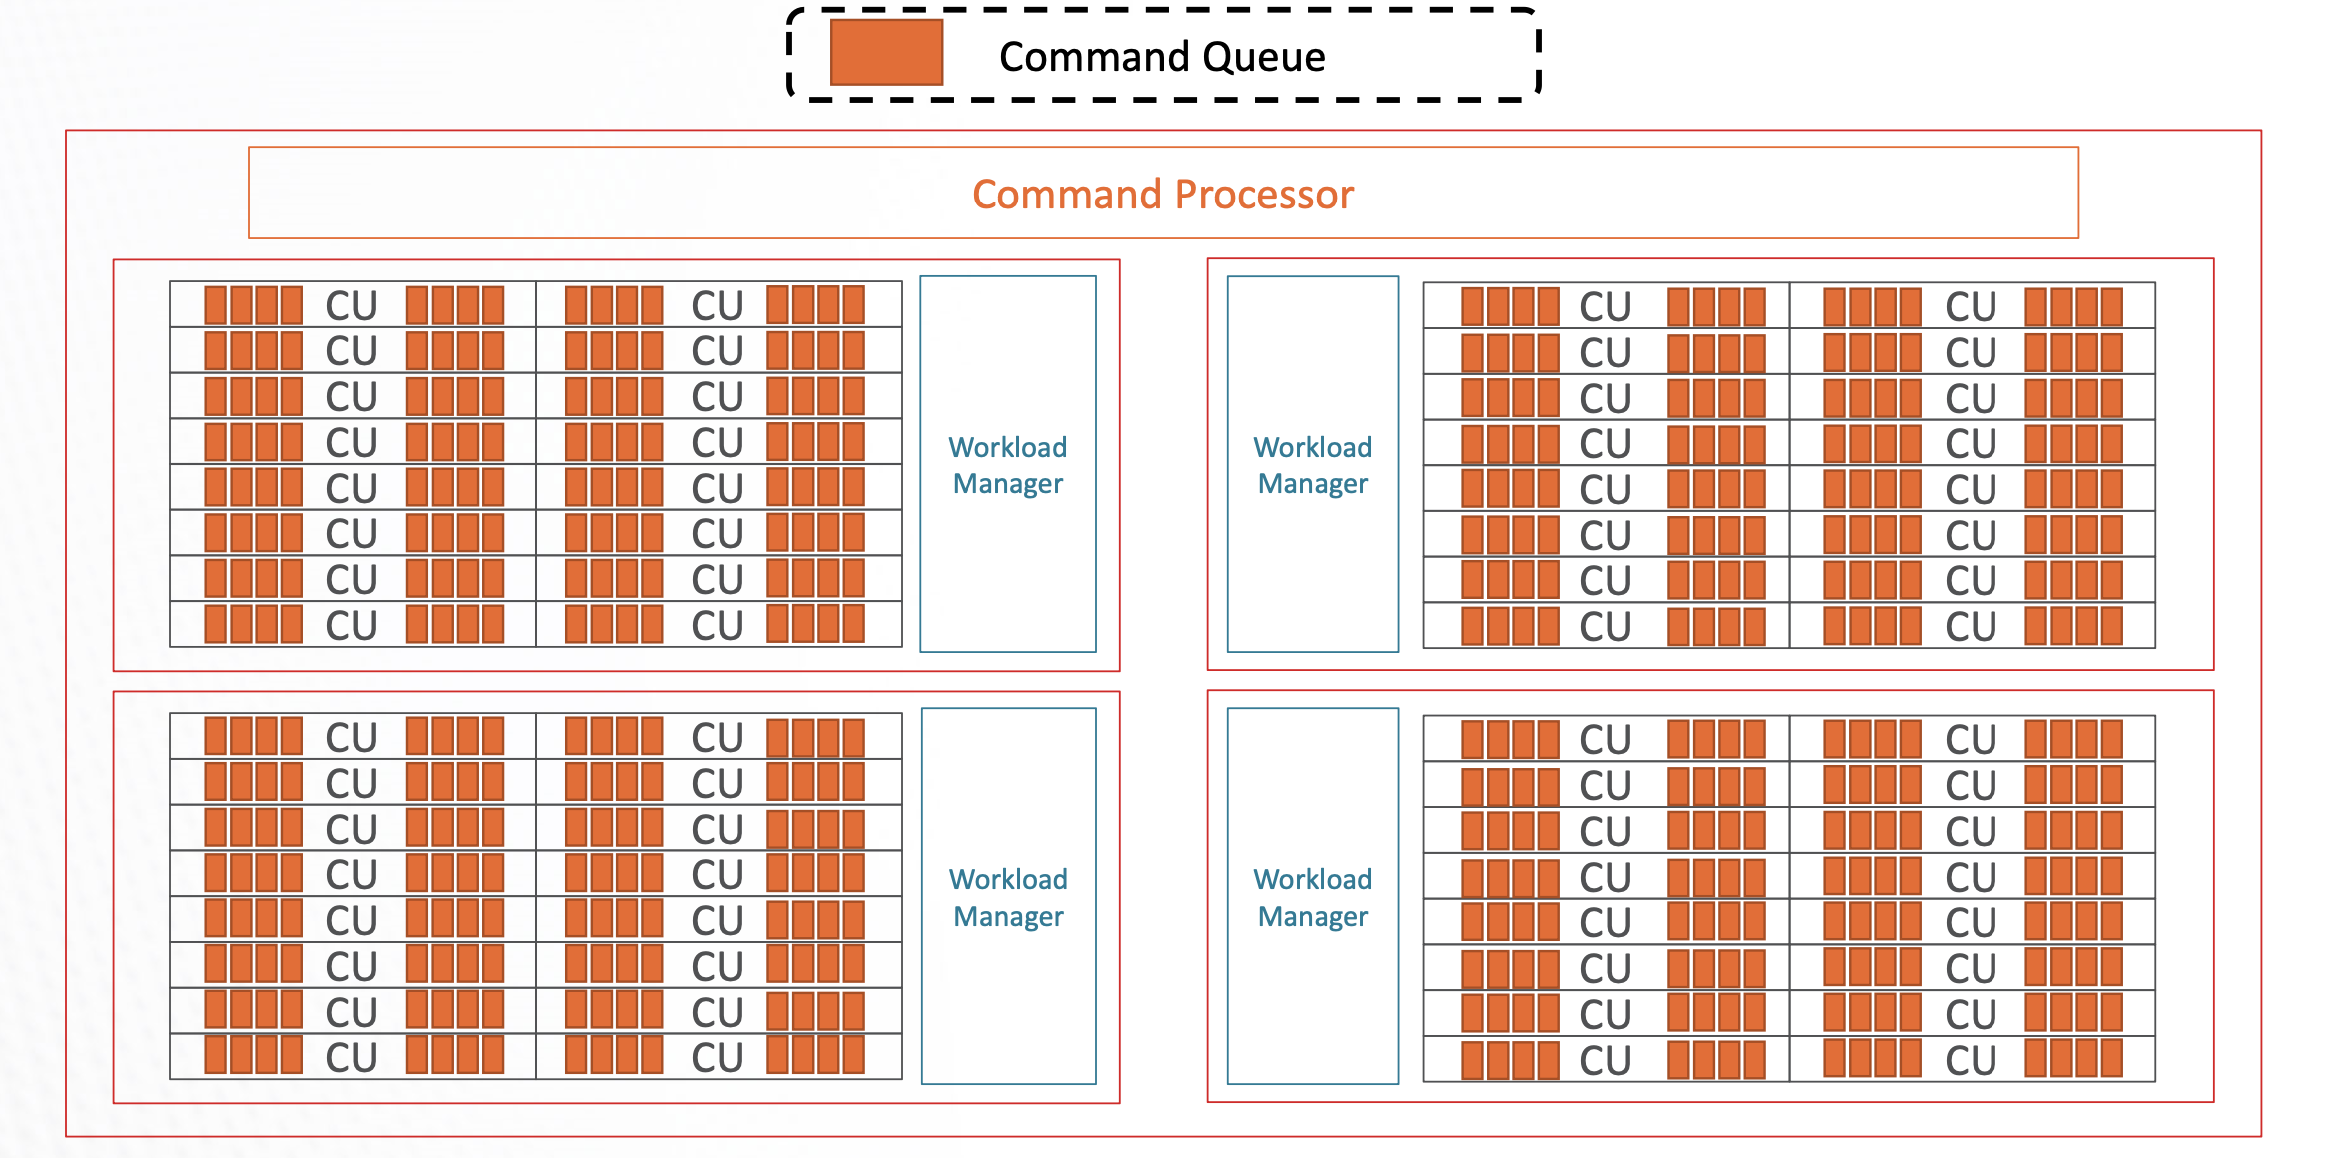
\includegraphics[width=\textwidth]{figures/gcn2.png}
\centering
\caption{A GCN-based AMD GPU that groups Compute Units into Shader Engines that are each managed by a Workload Manager \cite{amdConferenceTalk}.}
\label{gcn2}
\end{figure}

\quad Threads within a GPU are not scheduled individually. Instead, threads are grouped into units called wavefronts on AMD devices or warps for CUDA devices. Wavefront size is a property of the hardware architecture. They are 64 threads wide for GCN-based architectures, for example, or 32 threads wide on NVIDIA's CUDA-capable architectures. Wavefronts are executed on a single SIMD in four consecutive cycles. A one-cycle instruction therefore is executed in four batches across the each of the four 16-lane-wide SIMD units to cover all 64 lanes in an AMD wavefront. This hierarchy of CUs, SIMD units, wavefronts, and threads is illustrated in Figure \ref{gcn1}. 

\begin{figure}[hbtp]
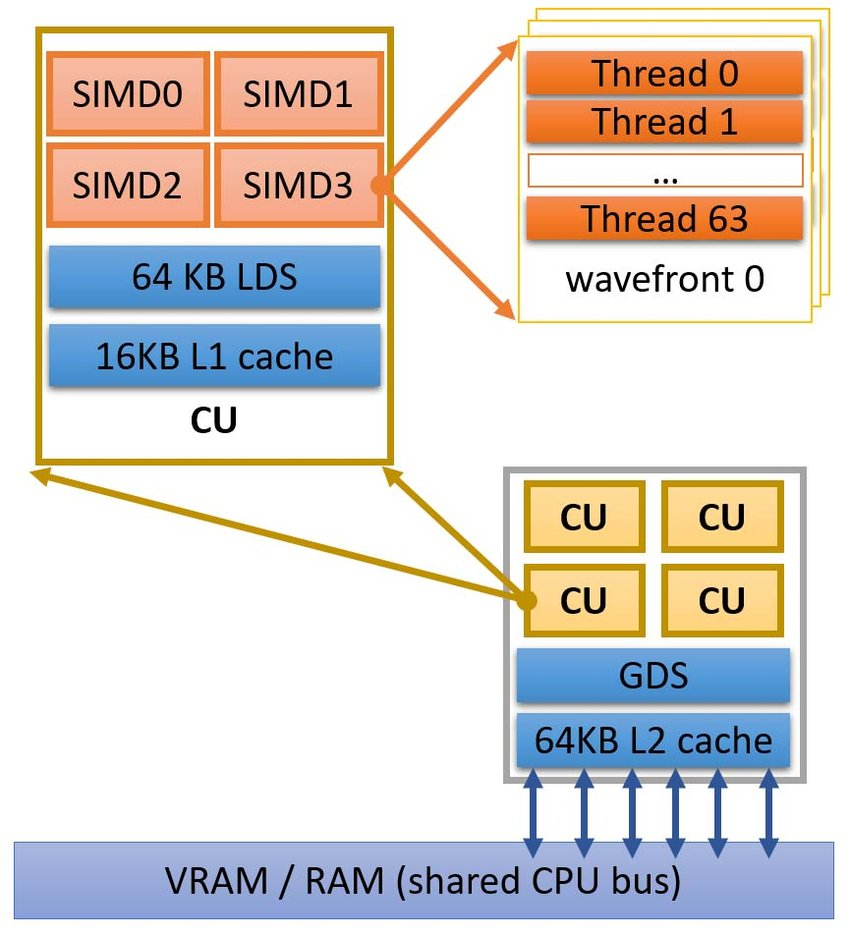
\includegraphics[width=70mm,scale=0.5]{figures/gcn1.png}
\centering
\caption{The contents of a Compute Unit is divided up into a group of resources and SIMD units that are each in turn separated out into wavefronts and threads \cite{gpuSortPerformance}.}
\label{gcn1}
\end{figure}


\quad GPU architectures are further complicated by their multi-tier hierarchy of memory. Visible to all CUs on the entire GPU is gigabytes of Graphics Double Data Rate (GDDR) synchronous DRAM and sometimes High-Bandwidth Memory (HBM) on newer devices. This memory is collectively referred to as `global memory'. When compared to CPU DRAM, the off-chip global memory for GPUs is designed for high bandwidth due to characteristics of the data commonly used for GPU acceleration. Unfortunately, global memory is still susceptible to longer latency times which is a fundamental property of the memory type \cite{greenBook, pycuda}. This latency can often act as a bottleneck for GPU acceleration. PCIe controllers help with the transfers across the PCIe bus with host memory, and some devices have Infinity Fabric Controllers that can manage communication with other GPUs on the system. The inclusion of DMA engines allows for asynchronous memory transfers between the device and the host, or between multiple devices. This layout of memory controllers and engines is illustrated in Figure \ref{gcn3}. At a finer level, each compute unit also has its own scratch-pad memory called the Local Data Share (LDS) which is typically 64KB for AMD and NVIDIA architectures. This data share is shared across SIMD units, and it can be used for communication between threads. Accessing shared memory is much faster than global memory, so a variety of techniques exist to help capitalize on this data share during execution time.

\begin{figure}[hbtp]
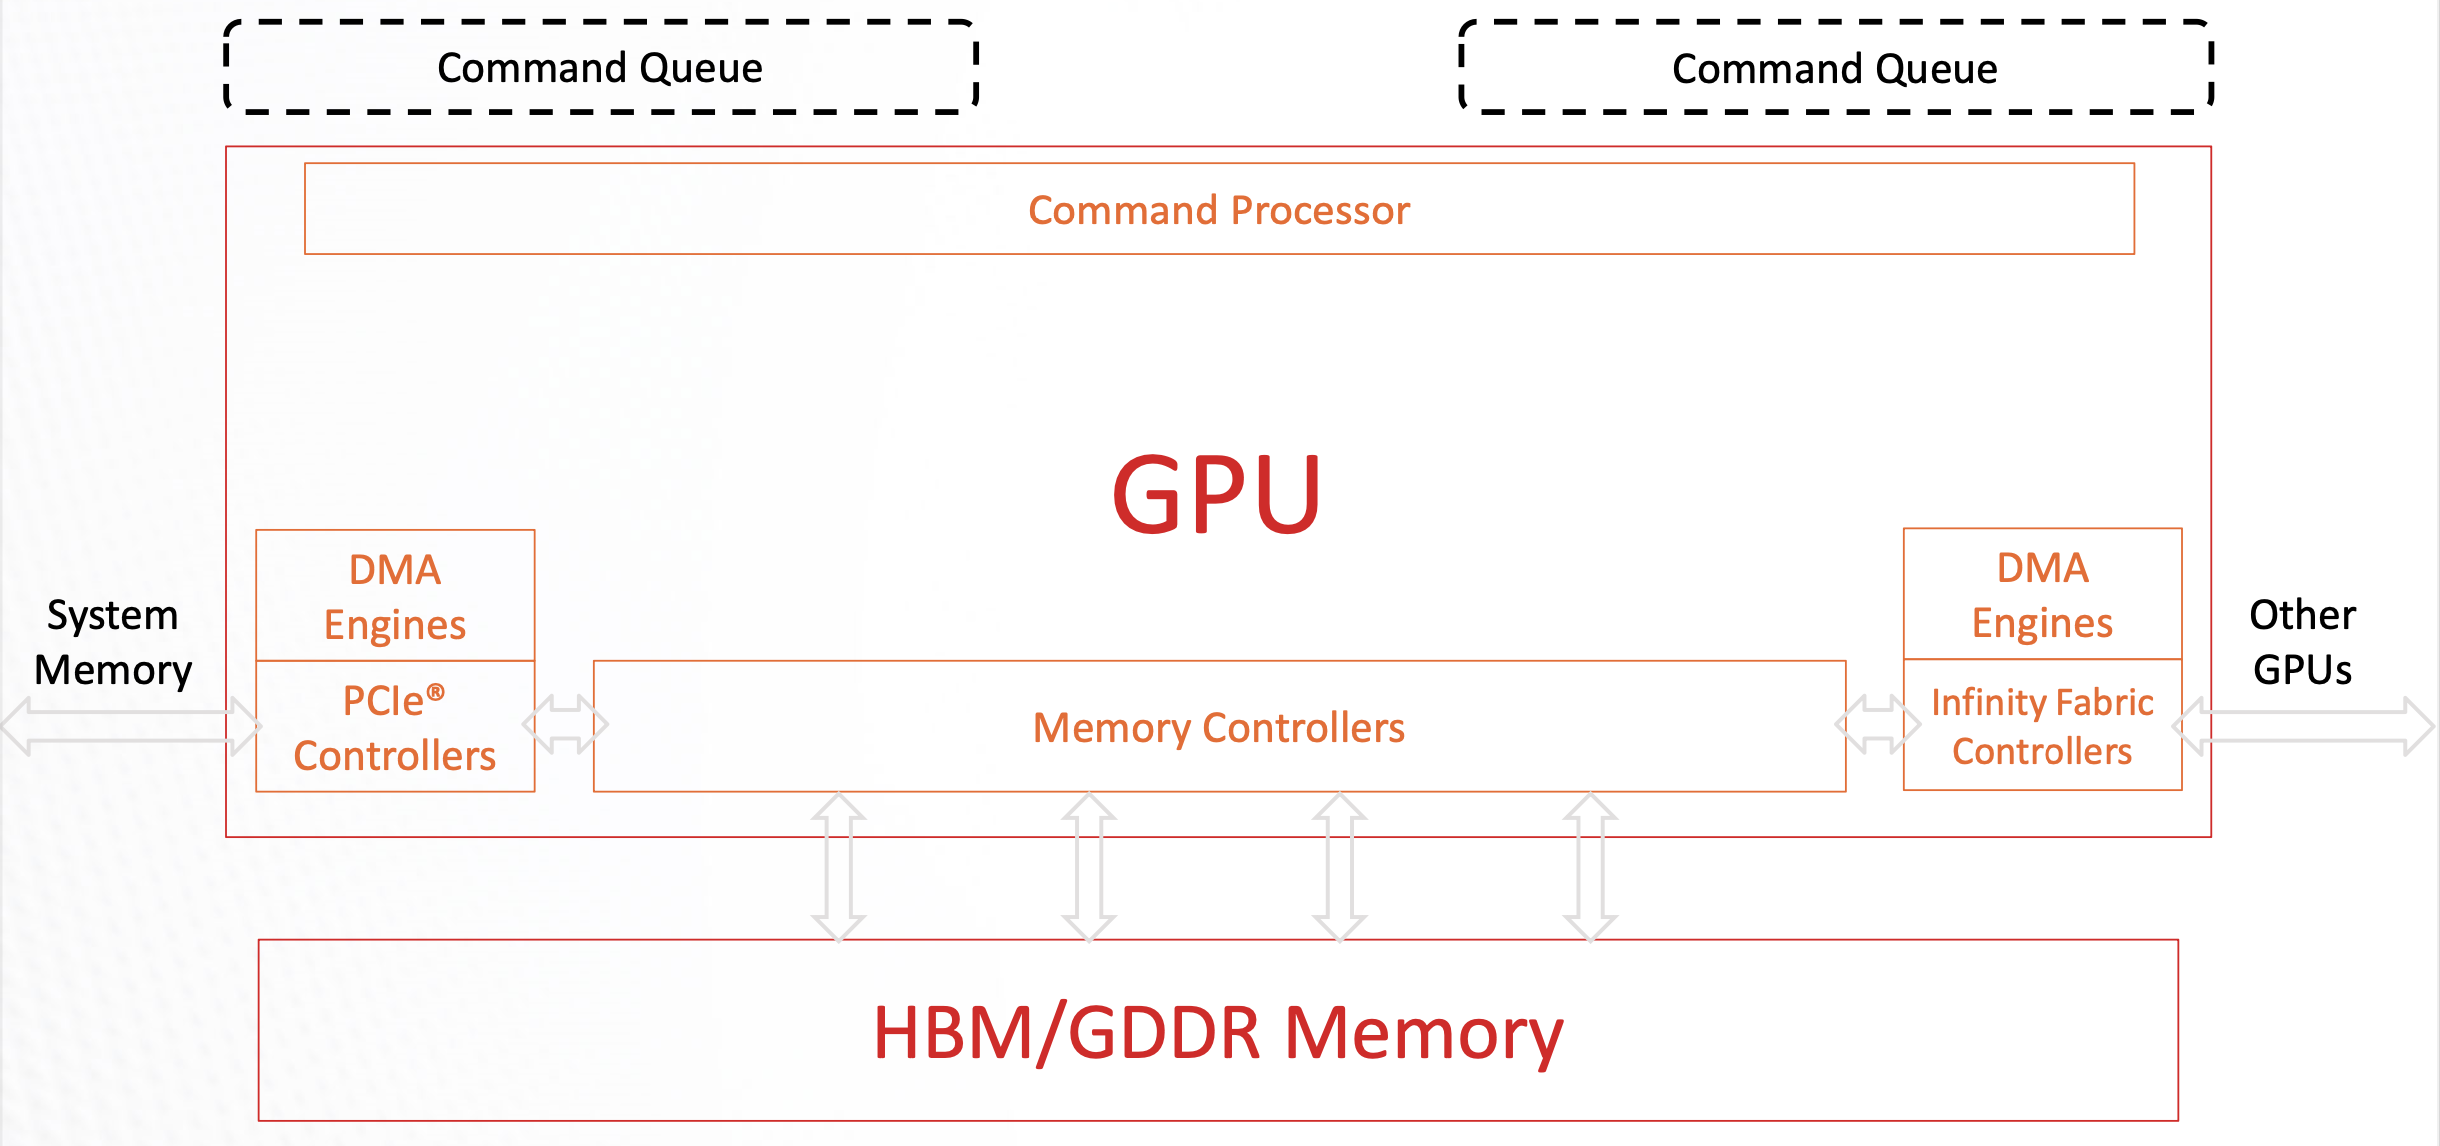
\includegraphics[width=\textwidth]{figures/gcn3.png}
\centering
\caption{A high level overview of the memory architecture on a GCN-based AMD GPU \cite{amdConferenceTalk}.}
\label{gcn3}
\end{figure}

\subsection{GPU Software}

When writing applications that must run on GPUs, code is split into two main parts — host code and device code. Host code is the normal part of an application that will run on the CPU and is written in a standard language such as C++. Device code on the other other hand are functions that are written to be run on SIMD units on a GPU. The entry point to device code sections are functions called kernels. Kernels make use of memory buffers that are allocated on the device from host code in order to manipulate a set of data. This means that most GPU-accelerated applications use a repeating pattern of allocating space on the device, copying data into the memory buffer, running a device kernel, and copying the data back to the host. 

\quad When GPU kernels are launched, they make use of the underlying architecture’s SIMD units to execute the work across many parallel workers which are often referred to as threads. These threads are organized into groups called workgroups on AMD devices or thread blocks on CUDA compatible devices. All threads within a workgroup exist on the device and the CU at the same time. These workgroups are made up of multiple wavefronts as discussed earlier, and GCN hardware uses 16 wavefronts per workgroup. Finally, workgroups are organized into a grid of multiple workgroup blocks as shown in Figure \ref{gridthreadblock}. The number and organization of the blocks and grid are under programmer control within the size limits allowed by the architecture. Blocks can be organized logically into 1, 2, or three dimensional grids, which is usually decided by the topology of the data. Kernels executing on images, for example, often work well as 2-dimensional grids. 

\begin{figure}[hbtp]
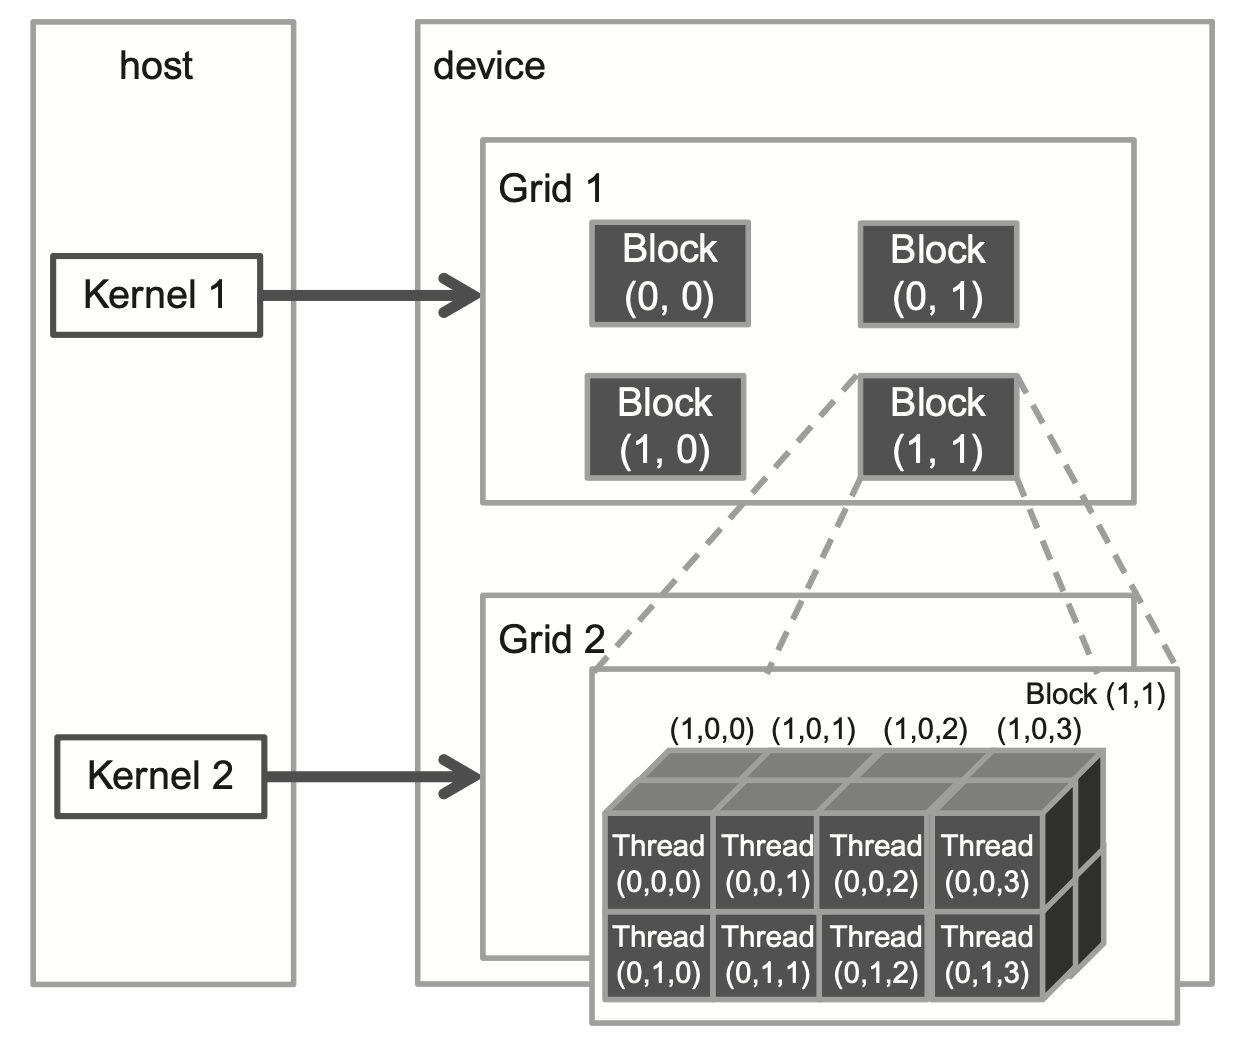
\includegraphics[width=100mm]{figures/gridblockthread.png}
\centering
\caption{GPU kernels divide data elements into logical groupings of grids, threads, and blocks \cite{greenBook}.}
\label{gridthreadblock}
\end{figure}

\quad The hierarchy of grids, blocks, and threads closely matches the organization of the underlying GPU hardware. Blocks are dynamically scheduled onto compute units, and all threads in a block execute on the same compute unit. This allows threads to share LDS memory and L1 cache. The downside to this hierarchy and memory model is that it provides an extra layer of complexity for the programmer. The parameters for the grid and block sizes must be chosen to make use of both the data and the device’s architecture, and kernel code should be designed to take advantage of faster LDS and cache memory when possible to avoid slower access to global memory. 

\quad The final software detail for GPU programming that needs to be discussed are streams. Streams are a way of dividing up the resources of the device for further parallel execution. Streams are queues of tasks that are guaranteed to complete in order on a given stream, and each stream is allowed to overlap and run synchronously with other streams on the same device. The exception to this rule is a special stream known as the null-stream. Tasks in the null-stream are not allowed to overlap with any tasks on any other stream. They only begin execution once all tasks enqueued on all other streams have completed. Blocking calls like memory copies will always happen on the null-stream.


\section{ROCm}

For a long time, NVIDIA has continued to dominate the GPU industry. As of Quarter 2 of 2021, NVIDIA is estimated to hold 83\% marketshare of the discrete GPU market over AMD's 17\% \cite{marketshare}. In the world of GPGPU computing, this dominance has come from its proprietary software included in the CUDA Toolkit which allows for the creation of GPU-accelerated software for embedded systems, workstations, data centers, cloud platforms, and HPC computers \cite{cuda}. This flexibility comes from its compiler, NVCC, which leverages the widely used LLVM infrastructure to allow developers to write kernels in modified syntax in C++ programs and compile them it for execution on NVIDIA devices \cite{nvcc}. On top of this, CUDA's early entry and dominance in the industry has given it the advantage of a strong community and ecosystem. The Radeon Open eCosystem (ROCm) is AMD's answer to CUDA which it describes as its ``open software platform for GPU-accelerated computing'' \cite{rocm}. Launched as part of AMD's ``Boltzmann Initiative'' in 2015, ROCm aims to solve new problems in GPU computing while maintaining an open source and multi-platform identity. This new ecosystem provides a wide range of programming models and languages to choose from. Among those is a C++ dialect called HIP (the Heterogeneous-Computing Interface for Portability) that provides many APIs and interfaces that mirror CUDA's \cite{hip}. It even includes a tool called HIPify that does most, if not all, of the work in converting CUDA programs to HIP. Unlike CUDA which is exclusive to NVIDIA devices, HIP allows for portability across platforms at the expense of a few API limitations \cite{hipfaq}.

\begin{figure}[hbtp]
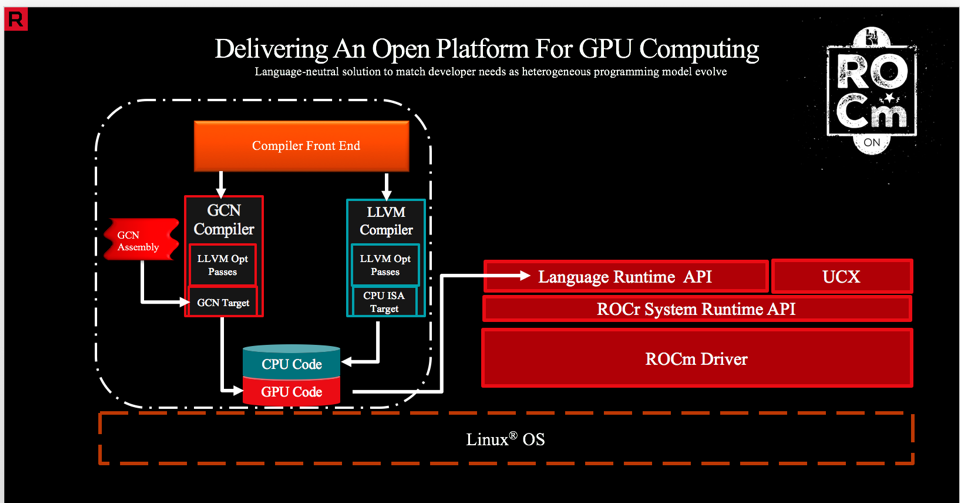
\includegraphics[width=\textwidth]{figures/ROCm_Stack.png}
\centering
\caption{An overview of the various systems in place that make up ROCm's foundation including compilers for both GCN and LLVM-based device runtimes \cite{rocmDocs}.}
\label{rocm1}
\end{figure}

\quad ROCm uses what is called the ROCr runtime which itself is based on the Heterogeneous System Architecture (HSA) Runtime API. The runtime is language-independent which allows it to serve many GPU-compatible languages including AMD's Heterogeneous Compute Compiler (HCC) which provides full control over AMD devices, or the Heterogeneous-Computing Interface for Portability (HIP) which specializes in cross-platform compatibility with both AMD and NVIDIA. To service these languages, the ROCm stack includes both GCN and LLVM compiler toolchains to compile GPU code for all compatible devices. This setup is illustrated in Figure \ref{rocm1}. ROCm also provides a variety of tools for supporting multiple GPUs. The ROCK kernel itself ROCm includes what is known as ROCmRDMA. It allows third party kernel drivers to use direct GPU memory access (DMA) and for DMA-based peer-to-peer data exchanges between devices using PCI express. ROCm also uses the Unified Communication X (UCX) library for both inter-node communication and intra-node communication, as well as the the open source message passing interface OpenMPI. 

\section{Python}

\subsection{Python language}

Python is a dynamically-typed high-level scripting language that has become increasingly popular in recent years. According to Stack Overflow's 2021 Developer Survey, Python gained in popularity over the previous year to become the 3rd most popular language of 2021 with more than 48\% of developers saying they use Python, and the sixth most loved language with more than 67\% of developers expressing interest in continuing to develop with it \cite{soSurvey}. Python has become immensely popular in areas of computing such as machine learning, data analytics, and scientific computing. One of the biggest advantages Python provides is its high level of abstraction and low-verbosity that makes it one of the most concise programming languages -- even when compared with functional languages \cite{rosetta}. This can allow for developers to focus more on high-level designs and processes and less on syntax \cite{pycuda}. When it comes to scientific computing, for example, it has been shown that Python's high level interfaces can help reduce the amount of time that scientists and researchers have to spend writing code \cite{gpucomppy}. 

\quad Python also comes with the advantage of a large compute-ecosystem and many open source libraries available for developers to use. Many libraries for scientific computing have historically been focused on raw performance and achieve this through lower level languages such as Fortran, C, and C++ \cite{pythonEcosystem}. Performance and ease-of-use do not have to be mutually exclusive, however. More recently, library designers have been writing performance-driven code in existing lower-level languages while designing interfaces for this code in a thin layer of Python function-wrappers. The language Python is now becoming synonymous with its massive collection of community-driven libraries and frameworks that tackle just about every computing need imaginable. The most popular of which are open source, open for contributors, and free for programmers to use.



\subsection{CPython}

CPython is the original reference implementation of the Python language. As the name suggests, CPython is implemented in the language C. This is the reason it is so easy for developers to extend the Python language through extension modules written in C or C-compatible languages. Although Python is often described simply as an interpreted language, the CPython implementation includes both a compiler and an interpreter. The compiler generates an AST from the Python source code and compiles it down into bytecode instructions. This bytecode gets executed by CPython's stack-based virtual machine as a giant evaluation loop that terminates once the Python program should stop for any reason.

\quad A very important part of the CPython runtime to understand is the way it handles concurrency. When it comes to maintaining thread-state, the CPython interpreter was created with what is known as the "Global Interpreter Lock" or GIL. It imposes the restriction that only one thread within a given Python process is allowed to process Python bytecode at a time. This means that multi-threading is often restricted to tasks such as IO operations that don't require access to CPython objects, functions, or memory, which all require the GIL to be held \cite{cpythonthreads}. Python programmers often have to turn to multiprocessing to achieve parallelism. Since each process runs in its own instance of the Python interpreter and occupies its own region of memory, each Python process has a distinct GIL instance.

\quad One of the next distinct features of CPython is how it handles Python types. Its easy to generalize Python by saying the language has no types. But in reality, within the CPython implementation, everything has one type -- the ``Python Object'' type. All values, error types, functions, and more are represented as objects that can be stored and passed around. To make this more confusing, every Python object has to be carefully reference-counted for the Python garbage collector to work. When an object is shared or duplicated, this count is incremented. Each time a reference is no longer needed, this count is manually decremented within CPython code. Once the count reaches zero, the Python interpreter knows that the object is no longer needed and its resources can safely be de-allocated. 
\chapter{Related Works}

\section{NumPy}

NumPy is an open source library that has become fundamental to scientific computing in Python. Its main contribution to the language is the \verb|ndarray| object representing a multi-dimensional array that can contain a variety of supported data-types. Since NumPy was developed in C, NumPy contains a range of useful C API tools that allow for other extension modules to take advantage of its functionality \cite{numpyCApi}. Today, NumPy is the backbone for countless scientific and mathematical libraries that build on \verb|ndarray|s and NumPy functionality. 

\quad One of the biggest draws for NumPy is its speed and efficiency. Without NumPy, Python programmers are limited to the built-in Python list which grows dynamically and can support content of mixed data types. NumPy arrays on the other hand are able to achieve better performance through constraints that allow them to behave like arrays in languages like C. NumPy's \verb|ndarray| objects can only contain a consistent data type, and arrays must maintain a fixed shape and size \cite{arrayNumpy}. Using these constraints, operations can be optimized and parallelized to efficiently act on the sequence of data. NumPy uses the idea of vectorization for its operations which are built on pre-compiled C code \cite{numpyDocs}. These vectorized functions ``broadcast'' operations across the entire sequence in a notation that is similar to what is seen in mathematics \cite{numpyDocs}. This improves readability by removing the need for explicit loops and iteration within Python.

\section{SciPy and Scikits}

SciPy is a library that has become the standard for modeling and computing scientific problems in Python. SciPy is built on top of NumPy and the \verb|ndarray|, but it adds a variety of new data structures such as sparse matrices and k-dimensional trees \cite{scipy}. These, in combination with methods for manipulating and visualizing data, create an ecosystem for solving a wide variety of problems. Today, more than 100,000 different code repositories use SciPy as a dependency \cite{scipy}. For specialized tasks, SciPy introduced the concept of SciPy toolkits, or SciKits, that add on packages for SciPy. Each SciKit brings specialized functionality for a variety of use-cases. Among these are scikit-image for image processing and scikit-learn which has become the gold-standard for machine learning in Python \cite{scikits}.

\section{Numba}

Numba is a just-in-time (JIT) compiler for CPython that is written as an extension library so that the interpreter does not need to be modified or replaced. Numba specializes in accelerating functions that use \verb|ndarray|s, NumPy functions and operators, and loops. It includes function decorators such as \verb|@jit| that can be dropped in to existing code to make it easy to accelerate without needing to be rewritten. Internally, Numba uses the LLVM compiler infrastructure. Python bytecode is analyzed and turned into an intermediate representation called the Numba IR \cite{lessonsLearned}. From there, Numba will attempt to infer types and lower the code to LLVM so that it can be compiled into efficient machine code. This compilation happens during the runtime of an application when the decorated function is called, but it only has to happen once for each function written since the compiled version is stored in a cache. Because this code is compiled and does not incur the overhead of the Python interpreter, Numba is able to achieve speeds comparable to those of C programs.  

\quad Numba acceleration is not just limited to the CPU. Numba is able to take advantage of GPU acceleration by leveraging CUDA's version of the LLVM library, NVVM. Numba is even able to support ROCm-compatible GPUs by compiling code into HSA kernels and device functions following the HSA execution model \cite{numbaRocm}. Numba is not perfect, however. Due to Numba's high level of abstraction, details and tuning are lost in translation and Numba lacks support for features such as dynamic parallelism and texture memory \cite{gpucomppy}. Python applications using Numba usually reach between 50\% and 85\% performance of the equivalent C/C++ CUDA implementations on compute heavy workloads. \cite{lessonsLearned}.

\section{CuPy}

CuPy is an open source Python library that aims to bring GPU acceleration to NumPy and SciPy. CuPy includes a wide variety of accelerated functions including linear algebra operations, sorting, sparse matrices, and more. In many ways, CuPy can function as a drop-in replacement for NumPy by providing functions of the same names. Originally, CuPy was designed to support CUDA-capable GPUs and leveraged popular CUDA-accelerated libraries such as cuBLAS, cuDNN, cuRAND, cuSOLVER, and cuSPARSE. Now, CuPy has expanded into experimental support for the ROCm ecosystem, and it and uses the equivalent ROCm-based computing libraries \cite{cupyRocm}.

\quad One of CuPy's most versatile features is the ability for users to create their own GPU kernels. Code snippets can be created in C++ syntax that are compiled into binaries that can be cached and used in subsequent runs. User defined kernels have the flexibility to either perform element-wise operations on all items in the data, or reduction kernels to fold data using binary operators \cite{cupy}. This allows for powerful flexibility and more control over GPU execution from Python at the expense of requiring the programmer to know kernel code design in C++ syntax. Even using the built-in functions, however, CuPy programmers can see tens to 100s of times speedup over NumPy when playing to CuPy's strengths.

\section{PyCuda and PyOpenCL}

PyCUDA and PyOpenCL are two open source toolkits built on CUDA and OpenCL respectively. They take the approach of using runtime code generation (RTCG) in order to take advantage of GPU parallelism from within Python code. RTCG works off of the idea of ``metaprogramming'' where code is tasked with interpreting and creating different sets of code to solve a problem \cite{pycuda}. In the case of PyCUDA, CUDA kernels can be written as strings within the Python code that are compiled at runtime using the NVCC compiler and run on the GPU as a binary. The compiled GPU code can be cached for future re-use which increases the efficiency of the application on subsequent runs. By extending support to OpenCL, PyOpenCL is able to work across a variety of platforms independent of the GPU manufacturer. 

\quad PyCUDA and PyOpenCL use a variety of techniques to tune the generated code. Loop slicing helps preserve locality of data access and use cache memory efficiently. The code can also can also adapt based on the amount of on-chip user-managed memory as well. Finally, tuning is performed based on available DRAM bandwidth. Although PyCUDA and PyOpenCL reduce the overhead of writing applications in pure C, C++, and CUDA, the programmer still needs to be familiar with the creation of GPU kernels in order to write the code templates within the Python program. This is not unlike kernel generation mechanisms in other libraries such as CuPy.

\section{TensorFlow}

TensorFlow is one of the most prevalent libraries for developing and training machine learning models, specializing in deep neural networks. It is compatible with a variety of architectures allowing TensorFlow to be deployed on CPU, GPU and TPU-based environments \cite{tensorflow}. It is also extremely flexible when it comes to the scale of the system it is deployed on. TensorFlow can run on devices as small as mobile phones or embedded devices, and it can scale up to run on large scale distributed systems with thousands of compute devices \cite{largeScaleTensorflow}. This makes it a powerful tool for a variety of machine learning fields such as speech recognition, natural language processing, computer vision, and more. TensorFlow also fits in very well with Python's library ecosystem. It is built around a multi-dimensional array type called a tensor, which are comparable to NumPy's \verb|ndarray|s, and these tensors are even compatible with NumPy operations. 


\section{Keras}

Keras is a high-level API for neural networks that is built on top of TensorFlow and other supported backends. Its interface is designed to be as simple and flexible as possible, allowing its users to quickly prototype and create deep learning models. Keras is built around two data structures called models and layers. At its most simple level, a sequential stack of layers are combined together to create a sequential model. More complicated models are built around arbitrary graph topologies that can handle a wide variety of machine learning problems \cite{keras}. 
\definecolor{dkgreen}{rgb}{0,0.6,0}
\definecolor{gray}{rgb}{0.5,0.5,0.5}
\definecolor{mauve}{rgb}{0.58,0,0.82}
\definecolor{backcolour}{rgb}{0.95,0.95,0.92}

\lstset{
backgroundcolor=\color{backcolour}, 
  language=C++,
  aboveskip=3mm,
  belowskip=3mm,
  showstringspaces=false,
  columns=flexible,
  basicstyle={\linespread{0.8}\small\ttfamily},
  numbers=none,
  numberstyle=\tiny\color{gray},
  keywordstyle=\color{dkgreen},
  commentstyle=\color{blue},
  stringstyle=\color{mauve},
  breaklines=true,
  breakatwhitespace=true,
  tabsize=3,
  escapechar=\&
}

\chapter{Implementation}

Millipyde intends to provide a framework for Python developers to accelerate tasks workloads transparently on cross-platform ROCm compatible GPUs. To do this, Millipyde is written as a C/C++ Python extension module that uses HIP for device code sections. Through its Python interface, Millipyde exposes two new types to developers to use - the \verb|gpuarray| and \verb|gpuimage|. These types can be used directly for a variety of functions. In addition, Millipyde also gives programmers three new GPU-workflow specific constructs to help tackle a variety of problems - the Operation, the Pipeline, and the Generator. This section explains the implementation and design of the Millipyde module itself as well as the two types and three workflow tools.

\quad The code is split into two main parts. The first are the functions that are exposed to Python when importing Millipyde as a library. For the rest of this chapter, we will refer to these as the API functions. Within the codebase, these function names are given the ``Py'' prefix. The other functions are those that are internal only to Millipyde and are not exposed to Python developers. We will refer to these as backend functions.

\quad All of Millipyde's functionality is validated using a large suite of test cases built on Python's \verb|unittest| framework. These test cases used an AMD Vega 10 XTX (gfx900) GPU. Two of these GPUs were used together in test cases that relied on multi-GPU execution. To confirm cross-platform capabilities, these unit tests are were also run on an NVIDIA Titan X (GP102) GPU. The full code repository is available with an MIT license at \verb|https://github.com/jasbury1/millipyde|. Millipyde also has a Docker container available for use at \\ \verb|https://hub.docker.com/repository/docker/jasbury/millipyde|.

\section{Millipyde C-Extension Module Design}

To build Millipyde as a Python extension module, it makes use of the library \verb|Setuptools|. The setup entry-point, \verb|setup.py|, builds a module object by specifying all of the C/C++ files as well as any included header directories. A partner file, \verb|setup.cfg|, contains project-specific metadata such as Millipyde's version, documentation, description, author, and more. \verb|Setuptools| by default will use the C and C++ compilers specified by the ``CC'' and ``CXX'' environment variables for any extension module files. These are overwritten by the Millipyde build system to instead point to the system's copy of the hipcc HIP compiler. Additional build scripts set the \verb|HIP_PLATFORM| environment variable to \verb|amd| or \verb|nvidia| based on the system we are compiling for. If we are compiling for an AMD system, the \verb|amd| value is used which directs HIP to use its clang-based compiler and the ROCclr runtime. If set to \verb|nvidia|, it instead uses an nvcc-based compiler and the CUDA runtime. 

\subsection{Error Handling}

Python has two types of errors that can occur -- syntax errors and exceptions. Syntax errors are errors in the parsing phase of the program such as missing characters or invalid white-space. All other errors that can happen during runtime fall into the second category of exceptions. When an exception occurs, it comes with two pieces of information: the exception type and a message of explanation. An example is the `ZeroDivisionError' which provides the concise message "division by zero." Since Millipyde is written in C and C++, a wide variety of different errors can occur. Most of these are to do with misusing types or memory. To make errors easy to understand from developers using Millipyde, the framework has an error handing system to turn almost all failure points into Python-accessible exception types with easily-understood error messages.

\quad Inside the extension module's backend, Millipyde has an \verb|enum| type called \verb|MPStatus| that enumerates every supported exception. An effort is made to ensure almost all backend functions return an \verb|MPStatus| value if it is reasonable to assume a failure could occur. From the Millipyde API functions, these status values are read and tested. If the status is not a success value, the status can be converted into an error string using \verb|mperr_str|. Python's thread error indicator is set to this string's value along with the type of exception. From here, the API function can return an indicator value (usually NULL) to signal to the interpreter that an error has occurred and to throw the stored exception.

\section{Device Management}

\subsection{Device State Data}

When the Millipyde module is initialized, it does a pre-processing step of analyzing the devices that are in the system. It starts by querying the ROCm runtime for the number of devices that are accessible. If there is more than one device, Millipyde creates a special data structure called the \verb|peer_access_matrix|. The pre-processing step tries every combination of two unique devices on the system and determines whether or not peer-to-peer data transfer is possible between them. If so, the associated bit in the matrix, whose row is represented by the first device and column represented by the second device, is flipped to be a 1. This makes it fast and easy for future functions involving data transfer to tell if it should try a peer-to-peer transfer. If peer-to-peer is not enabled, these functions will default to using slower transfers using the CPU main memory as an intermediate between the two devices. It's important to note that peer-to-peer access will only be supported if large-BAR address modes are enabled for the GPUs in the system BIOS. In addition to setting up any necessary data structures and populating the \verb|peer_access_matrix|, the pre-processing step will attempt to find the best device available. It does this by iterating through all available devices to find the device with the highest metric $(mcu * mcf)$ where $mcu$ is the maximum number of compute units and $mcf$ is the maximum clock frequency. The result is stored as a variable called the \verb|recommended_device|.

\quad In addition to maintaining a variable for the recommended device, Millipyde's device manager also maintains a variable called \verb|target_device|. This is the device that was explicitly specified as the device to use by the user in Python. If we are in a scope where no target device was specified, this variable defaults to the macro value \verb|DEVICE_LOC_NO_AFFINITY| which means that Millipyde can schedule it on any device available. In most cases, this will be the \verb|recommended_device|. There is one more case in which \verb|target_device| will be ignored. GPU-compatible types such as \verb|gpuarrays| and \verb|gpuimages| can be `pinned' to a device meaning that kernels using that object will only operate on the device they are `pinned' to, regardless of what device is targeted for the given scope. This feature is not exposed to Python. It is only used internally to Millipyde for workflow constructs that are executed on a specific device. This will be discussed later in more detail. The general algorithm is shown in Algorithm \ref{alg:moving}

\begin{algorithm}
\caption{The decision algorithm for moving an object o to a different logical device for future kernel execution.}
\label{alg:moving}
\uIf{$o$ is pinned to device $d$}
{
    \uIf{$o.location \neq d$ }
    {
        $o.location \gets d$\;
    }
}
\uElse
{
    \uIf{$target\_device \neq DEVICE\_LOC\_NO\_AFFINITY \And o.location \neq target\_device$ }
    {
        $o.location \gets target\_device$\;
    }
}
\phantomsection
\end{algorithm}

\quad The final data structure that Millipyde's device manager uses is an array of \verb|MPDevice| structures which are pictured in Figure \ref{mpdevice}. These structures have a boolean value for whether or not each enumerated device is usable or not. Millipyde does a sweep through all detected devices during the module initialization phase and attempts to use each device. If the device is not useable for any reason, the respective \verb|MPDevice| structure is registered as invalid. Millipyde will never schedule any operations on unusable devices. In addition, it will throw an exception if the user attempts to set an invalid device as the \verb|target_device| from inside a Python program. 

\begin{figure}[hbtp]
    \begin{lstlisting}
    
    typedef struct mp_device {
        MPBool valid;
        hipStream_t streams[DEVICE_STREAM_COUNT];
        MPDeviceWorkPool *work_pool;
    } MPDevice;
    &\newline&
    \end{lstlisting}
    \caption{The definition for MPDevice.}
    \label{mpdevice}
\end{figure}

\quad \verb|MPDevices| help coordinate parallel kernel execution by maintaining the streams that have been created on each respective device. If many functions are attempting to launch parallel kernels in separate streams, its possible that synchronous execution on the CPU may become the bottleneck for performance. An example of this is demonstrated in Figure \ref{streamsAndThreads}. Because of this, each \verb|MPDevice| structure also maintains a pool of CPU threads equal to the amount of streams on the device. Each pool has a single queue through which work can be submitted and distributed to each of the parallel workers. These pools for each device are created at module initialization, and their threads remain idle while no work is en-queued inside of the work queue. 

\begin{figure}[hbtp]
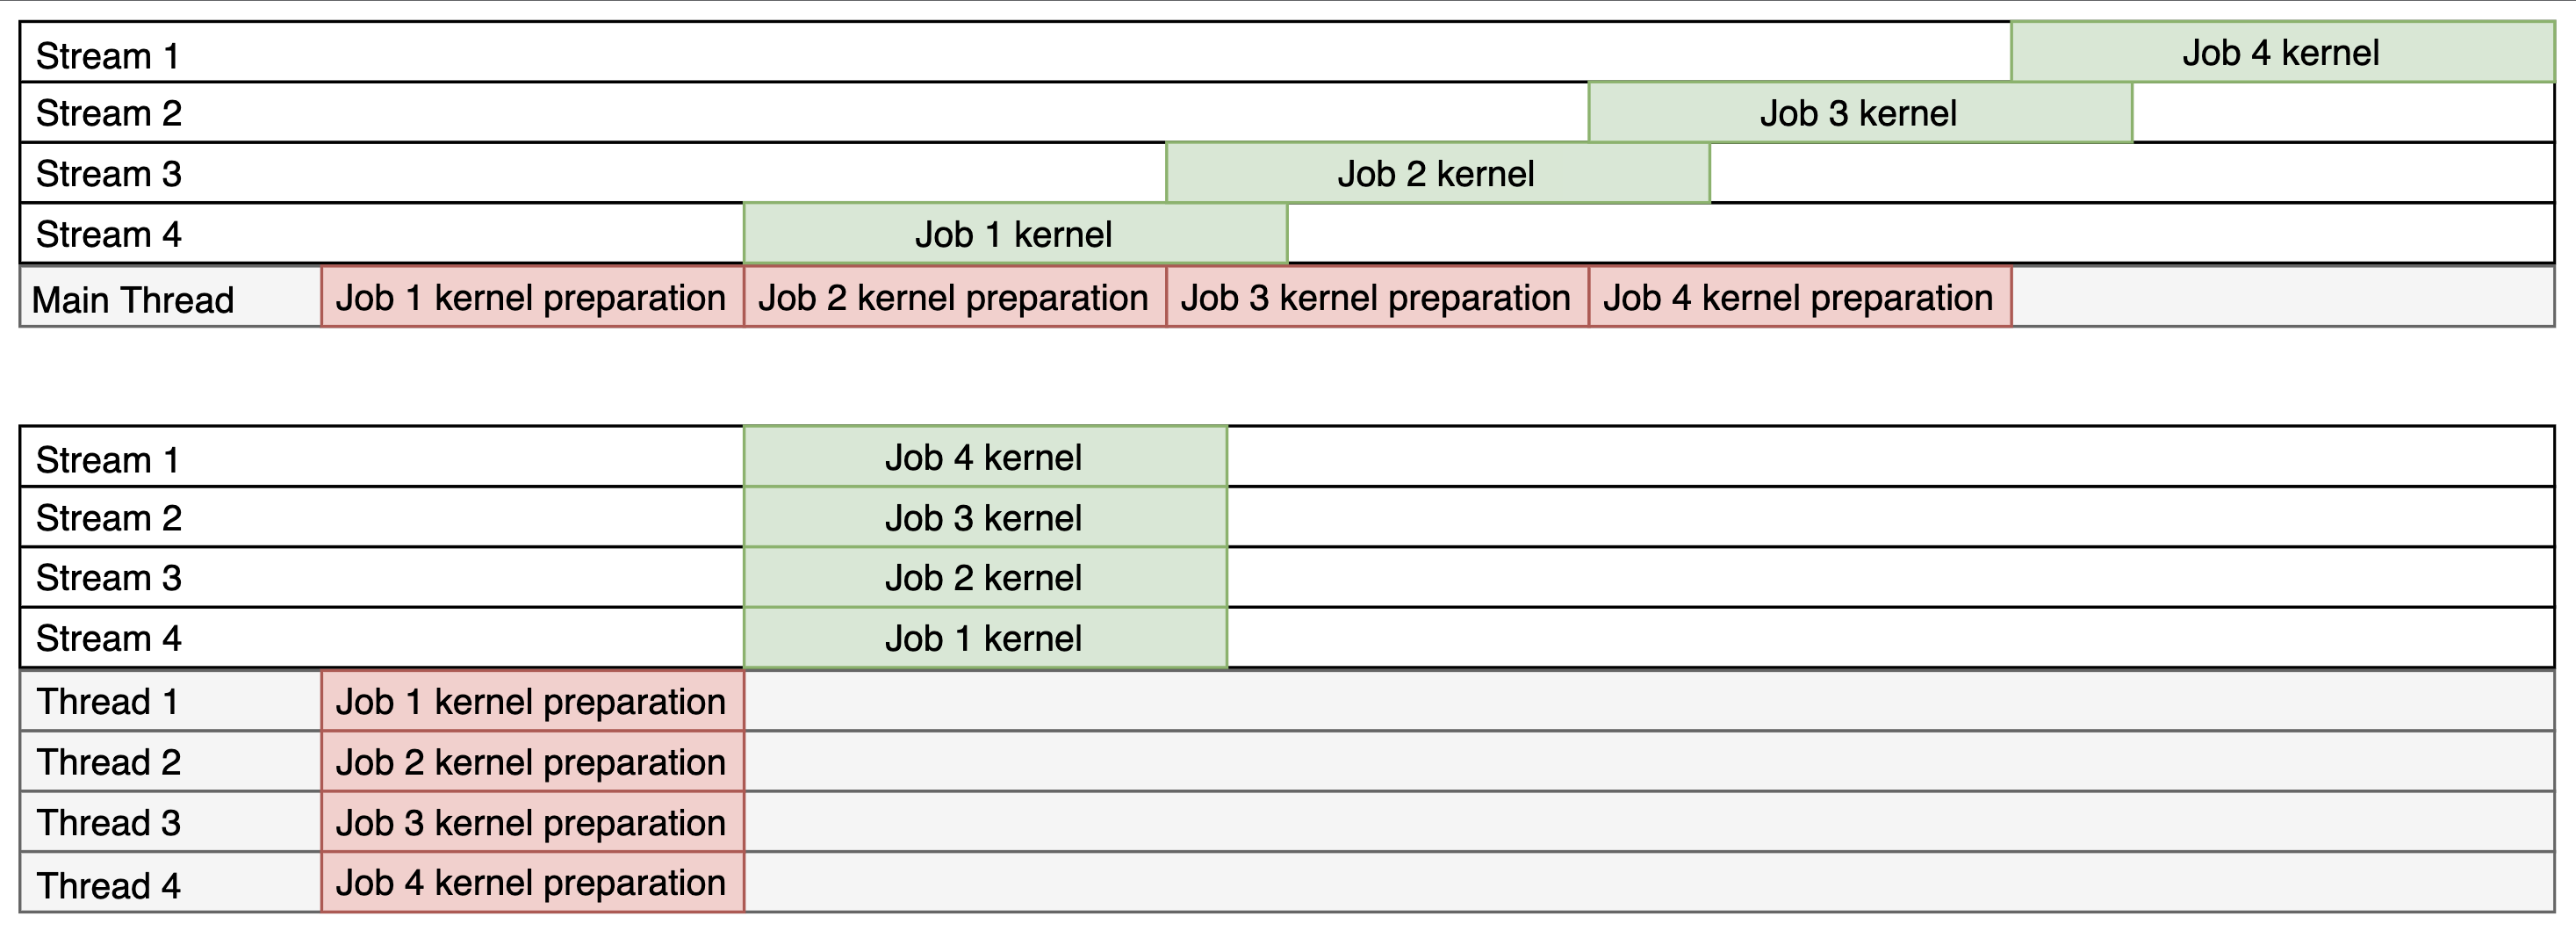
\includegraphics[width=\textwidth]{figures/streamsAndThreads.png}
\centering
\caption{Potential benefits to threading CPU work associated with parallel GPU streams.}
\label{streamsAndThreads}
\end{figure}

\quad Millipyde registers an exit function using the Python API call \verb|Py_AtExit|. This function guarantees that all allocated device data is freed such as the \verb|peer_access_matrix| and the array of \verb|MPDevices|. For each \verb|MPDevice|, all thread pools will be safely stopped and all threads and remaining work will be deleted. The exit function waits for all work in all streams to synchronize before destroying each stream. This function gets triggered regardless of how the Python code exited. By doing this, we are able to ensure safe cleanup of all data, even in the case of run-time exceptions.

\begin{figure}[hbtp]
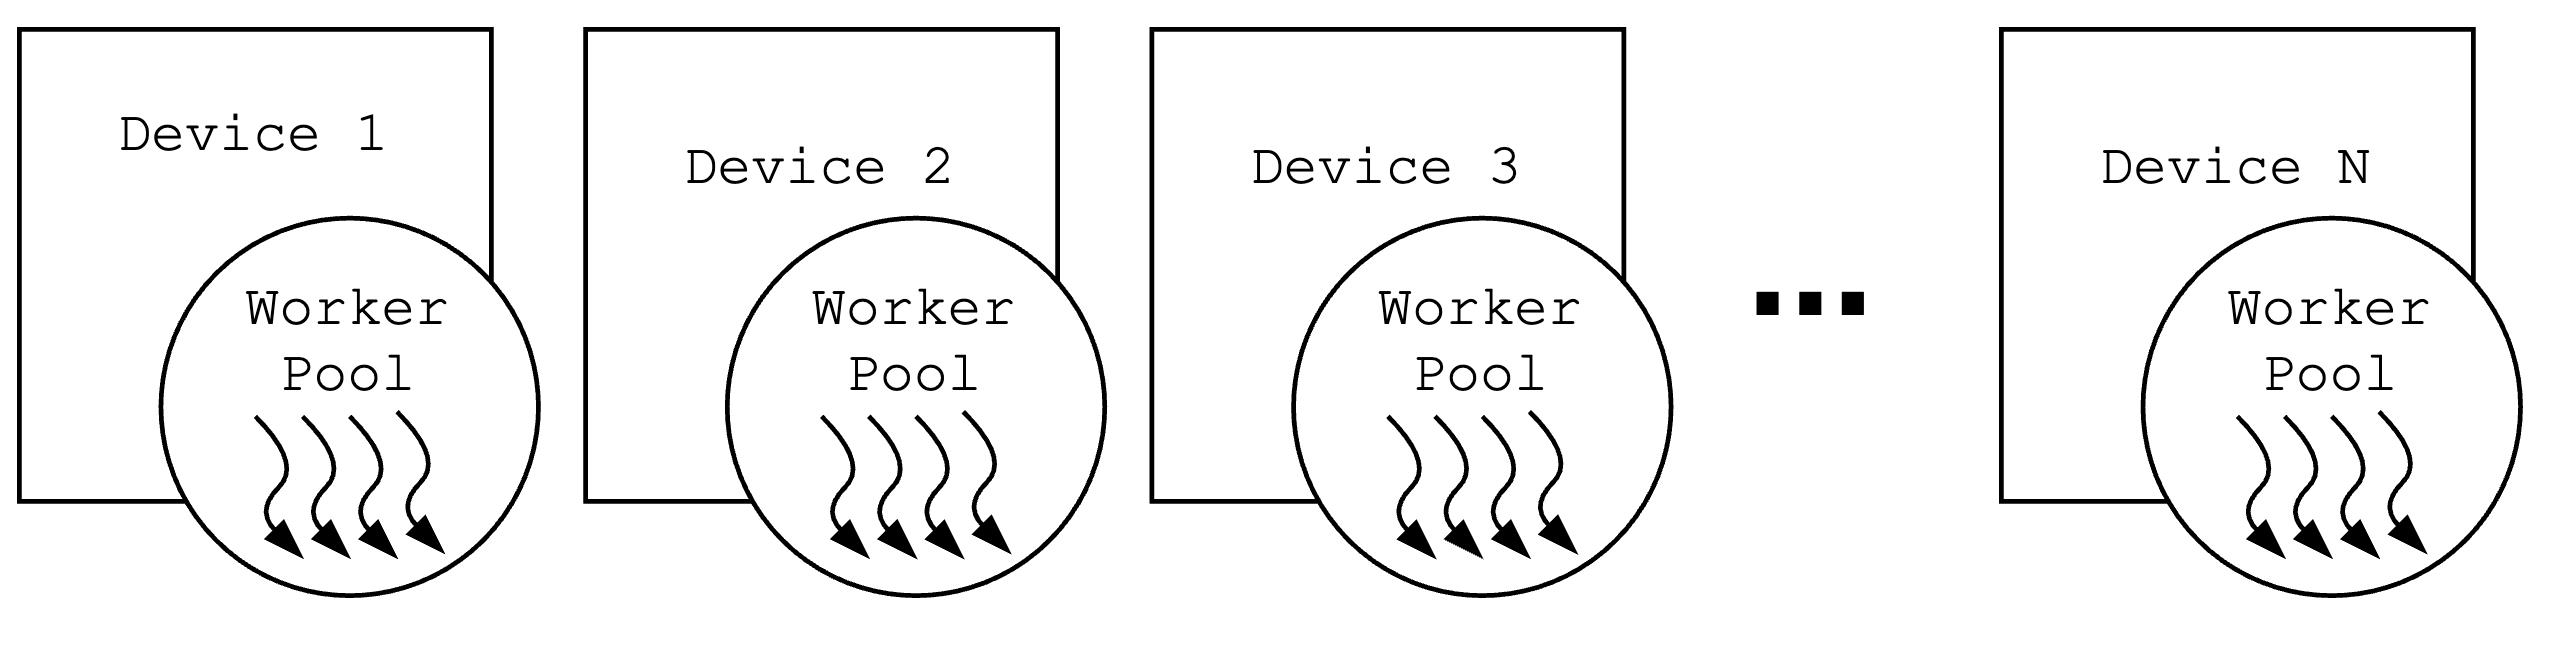
\includegraphics[width=\textwidth]{figures/devices.png}
\centering
\caption{A separate thread pool of workers is allocated based on the number of devices.}
\label{workers}
\end{figure}


\subsection{Device Object}

Millipyde uses a class called `Device' to control the device that is targeted for a specific scope. Each instance of a Device is known as a Python ``context manager'' to make sure values and state are only maintained for a specific scope. This is a common technique used in other libraries, and Millipyde's device context managers therefore look and function in a way that is very familiar to equivalent constructs in other GPU-compatible Python libraries such as CuPy. Millipyde's Device objects handle the context manager protocol by providing its own implementations of the special \verb|__enter__| and \verb|__exit__| methods. These methods are automatically compatible with Python's \verb|with| statements which allows them to set up a specific context at the start of the \verb|with|, and clean up the context when exiting the \verb|with| block or context. On entrance, the Device objects save the current \verb|target_device|, and switch it over to the new one specified. On exit, the Device will transition back to the previously stored \verb|target_device|. By doing this, scopes for specific devices can be nested along with each nested \verb|with| block. Examples of this can be seen in the API in Chapter 9.

\quad One of the main purposes of context managers in Python is making sure resources are properly released when a context is exited. This needs to happen both when the end of a context is naturally reached, and when an end of a context is prematurely reached due to an exception. Although no actual resource needs to be officially released for our device contexts, Millipyde still takes advantage of this functionality to change behavior based on whether the context's execution was successful. If it was successful, \verb|__exit__| will synchronize with the targeted device to make sure execution has fully completed before reverting the target back to the previous device. If an exception occurred within the \verb|with| statement's context, the state of the target device is reset and the exception is passed along to the calling code. This reset includes deleting all streams, memory allocations, kernels, and events so that the device is left with a blank state for future use. Millipyde will then also reset and restore all managed data structures such as streams in the case of one of these exceptions. By doing this, users have the option to recover from a failure and still be able to use all of Millipyde's functionality.  

\section{GPU-Compatible Types}

Millipyde includes two types that are compatible with Millipyde's GPU-accelerated methods and constructs -- the \verb|gpuarray| and the \verb|gpuimage|. Collectively these types are referred to as Millipyde's GPU-compatible types. Between these two types, the \verb|gpuarray| contains most of the implementation details while the \verb|gpuimage| type is only a subtype of the \verb|gpuarray|. It inherits all of the same functionality, attributes, and array structure as the \verb|gpuarray|, but it adds on additional image-specific functionality and constraints. All \verb|gpuimages| are only allowed to be 2-dimensional arrays of doubles for greyscale images, or 3 dimensional arrays of 8-bit values for colored images. In these 3-dimensional arrays, the inner most dimension can either be three values wide for RGB or four values wide for RGBA. The \verb|gpuarrays| on the other hand are allowed to represent any number of dimensions which can be any chosen size. These two types are initialized using any existing array-like arguments. This includes, for example, the builtin Python list, or even NumPy's own \verb|ndarrays| or SciPy's \verb|ndimages|.

\subsection{NumPy compatibility}

Millipyde's \verb|gpuarrays| and \verb|gpuimages| aim to be the GPU-accelerated equivalents to NumPy's \verb|ndarrays|. Its important to note, however, that neither type is a subtype of the \verb|ndarray|. Although NumPy's C APIs do allow for subtyping, the \verb|gpuarray| and \verb|gpuimages| types distinct enough in their use-cases to warrant the creation of their own distinct types. They still maintain compatibility with NumPy, however, by registering appropriate conversion functions and following NumPy protocols for special functions. As mentioned previously, all \verb|ndarrays| can be converted into one of our GPU-compatible types by using it in the type's constructor. They can also be explicitly cast back into \verb|ndarrays| using NumPy's \verb|numpy.array| or \verb|numpy.asarray| functions. This is done by including our own implementation of the \verb|__array__| interface that Numpy uses for array testing and conversion. 

\quad For any NumPy-specific function calls, our types can be implicitly converted to \verb|ndarrays| as well to maintain compatibility. Both \verb|gpuarrays| and \verb|gpuimages| provide implementations of the NumPy protocols \verb|__array_function__| and \verb|__array_ufunc__|. When either a standard NumPy function or universal function is called, an \verb|ndarray|-equivalent copy of the respective \verb|gpuarray|/\verb|gpuimage| argument is created. The given function or \verb|ufunc| is re-called using the \verb|ndarray| argument, and the copy can be safely used and reused without worrying about mutability issues with the original \verb|gpuarray|/\verb|gpuimage|. To store the result back as our GPU-compatible type, we can re-call the \verb|gpuarray| or \verb|gpuimage| constructors using the result of the NumPy function. 

\subsection{MPObjData}

All \verb|gpuarrays|, and therefore \verb|gpuimages|, compartmentalize their data in a structure called \verb|MPObjData|. This data structure, as shown in Figure \ref{mpobjdata} contains \verb|pointers| any array data that is allocated on the device as well as the arrays dimensions, type, number of bytes, the device ID where the memory is located, and a boolean value for whether or not the data is `pinned' on a specific device. They also contain a reference to which stream is in use so that we know which stream to use in the case of sequences of streamed operations. As mentioned previously in this chapter, device pinning has no relation to actual pinned memory. It is a flag that means an instance of a type should only be operated on using a specific logical device, and should not be moved for any reason. While \verb|gpuarray| objects and \verb|gpuimages| are allocated on the Python heap, the \verb|MPObjData| objects that they hold references to are allocated on the standard process heap that is handled by the C library allocator using \verb|malloc()| calls. This is because some functions operate entirely in C-space and do not contain any references to Python functions, objects, or memory. By drawing a clear line between what data structures use Python data and which ones don't, Millipyde can more safely make assumptions about what functions and data can be operated on in threads that bypass the Global Interpreter Lock. 

\begin{figure}[hbtp]
    \begin{lstlisting}
    
    typedef struct {
        void *device_data;
        int ndims;
        int *dims;
        int type;
        int mem_loc;
        void *stream;
        MPBool pinned;
        size_t nbytes;
    } MPObjData;
    &\newline&
    \end{lstlisting}
    \caption{Encapsulated data associated with each GPU-type.}
    \label{mpobjdata}
\end{figure}

\quad The array data pointer stored in the \verb|MPObjData|, called \verb|device_data| as seen in Figure \ref{mpobjdata}, is copied to GPU memory as soon as the respective GPU-compatible type is created. This memory is left on the device across subsequent calls to GPU-compatible methods that operate on the object. This reduces the overhead of copying memory back and forth between the host and the device when multiple function calls are performed on the device. Since kernel calls on the GPU can run asynchronously, any functions modifying this memory can continue to run even after the Python API function causing the modification has returned. 

\quad Millipyde will synchronize with the GPU and copy the memory back to the host any time a function is called that works on the host rather than the GPU. This includes Numpy functions which automatically convert our GPU-compatible types to \verb|ndarrays| using \verb|__array_function__| or \verb|__array_ufunc__|. Users can also force GPU-compatible types to synchronize and copy back to the host by manually calling a conversion function to a host-based type such as Numpy's \verb|numpy.array| or \verb|numpy.asarray|. All of these functions go through the \verb|gpuarray| or \verb|gpuimage's| \verb|__array__| interface that is responsible for memory transfer and releasing of GPU resources. If this call mutated the only reference to a \verb|gpuarray| or \verb|gpuimage|, all GPU-based resources will be cleaned up and disposed of. If this was only one of many references to the object, a host-based copy will be created, and the original \verb|gpuarray| or \verb|gpuimage| will keep its GPU-based resources available for future kernel calls. All GPU allocations and resources are also safely freed when the respective object is deleted following its reference count reaching 0.

\subsection{MPFunc}

All methods that operate on GPU-compatible types are split into two parts. The first part is the API component that is written to be compatible with CPython's APIs and to be callable from Python. It handle's type checking, exception handling/throwing, and acts as a wrapper function for the second part which is referred to as an \verb|MPFunc|. \verb|MPFunc|s are the functions that actually operate on the \verb|MPObjData| for the GPU-compatible type that the method was called on. All \verb|MPFunc|s follow a standard format as shown in Figure \ref{mpfunc}. They return an \verb|MPStatus| value, and take in the pointer to the GPU-Compatible type's \verb|MPObjData| as well as a void pointer containing any other parameters needed. 

\begin{figure}[hbtp]
    \begin{lstlisting}
    
    typedef MPStatus (*MPFunc)(MPObjData *, void *);
    &\newline&
    \end{lstlisting}
    \caption{The definition for MPFunc}
    \label{mpfunc}
\end{figure}

\quad The reason behind this split is to provide a clean separation of concerns between the CPython API functions and the backend C/C++ functionality. By doing this, Millipyde can internally call the \verb|MPFunc| itself rather than going through the wrapping API functions. This is commonly done any time Millipyde uses CPU threads. Since \verb|MPFunc|s are internal only to Millipyde and never call CPython functions or use CPython data, they are safe to call internally without needing the GIL to be held. By following a consistent format with both the return type and parameters, pointers to \verb|MPFunc|s can be passed around and stored for all methods that operate on GPU-compatible types. This is done with the Pipeline objects that are discussed later in this chapter. These functions still have the flexibility of returning any of our defined \verb|MPStatus| value, and the wrapping CPython function can turn this status value into a Python exception for any status that is not \verb|MILLIPYDE_SUCCESS|.


\section{Execution Constructs}

Millipyde's types, the \verb|gpuarray| and \verb|gpuimage|, can be used in standalone functions to achieve acceleration on the GPU. An example of this is calling the included \verb|gaussian| blur function on a \verb|gpuimage| instance. For more complicated execution, such as performing lots of transformations on many objects or scheduling functionality across multiple devices, Millipyde includes several of what we will refer to as ``execution constructs.'' They include the Pipeline object, the Generator object and their building block the Operation object.

\subsection{Operation Object}

In Python, almost everything is represented as an object. This includes variables, classes, built-in functions, user defined functions, methods, and more. The last three of those all fall under the category `callable' representing objects that can be called. Internally in the CPython backend, a parameter called \verb|tp_call| in a given object's type structure holds a function pointer that gets used whenever a Python user calls a function, method, or other callable object. At a high level, Millipyde's Operation objects are wrappers around python callables that add extra data such as probabilities.

\quad Operations for all callables besides instance methods are constructed using the callable name itself, the parameters with which to call the callable with, and optionally a float parameter between one and zero representing a probability. A reference to the callable and a tuple object for the arguments all get copied to the Operation's internal memory so that they can be run one or more times using the Operation's \verb|run| method. Examples of this are shown in the API documentation in Chapter 9.

\quad Instance methods are handled in mostly the same way with one small difference. When constructing an Operation, the operation doesn't know what instance the instance method will be called on, or even what type the instance method is associated with. Because of this, Operations that represent instance methods are constructed with a string method name rather than the method name itself. These Operations can be invoked one or more times using the \verb|run_on| command, and run-time lookup is performed to find the corresponding method with a matching name from the instance's attribute lookup table. 

\subsection{Pipeline Object}

The goal of Millipyde's Pipeline object is to get a group of inputs all passed through a sequence of operations as quickly as possible. When instantiating a Pipeline, the user provides a Python list of GPU-compatible inputs (\verb|gpuarrays| and/or \verb|gpuimages|), a list of Operations to complete, and optionally a device ID of a GPU to perform execution on. If no device ID was specified when the Pipeline was created, then the Pipeline instance will defer to the \verb|target_device| at run-time when the Pipeline is executed. If no \verb|target_device| is set, the Pipeline will attempt to use all available resources to complete the operations.

\quad Pipelines work based on mutation. Because of this, executing a Pipeline does not return any specific output back to the user. Instead, the original list of inputs that were passed in will now be modified to include all of the transformations included in the list of Operations. This also means that the original size of the input set is left unchanged throughout execution.

\quad Pipelines take advantage of both CPU and GPU parallelization. Every input in the input set is grouped together with a device ID of the device to execute on, a stream ID of a stream to operate within, and its list of Operations. From there, they are sent to the work queue associated with each device to be picked up by the workers in the work pool. Once execution starts, the operations are applied to the individual input one-by-one on the same CPU thread and within the same GPU stream. If the input has memory on a different device than it is scheduled on, the memory only has to be transferred once and all operations can be completed on the newly assigned device. At most N inputs will be be processed per device where N is equal to the amount of CPU workers and GPU threads. A sample scheduling is shown in Figure \ref{pipeline}. In this example, the last three inputs will only be operated on once the respective thread/stream ID is free from the first batch on inputs that were scheduled on \verb|Device| 0.

\begin{figure}[hbtp]
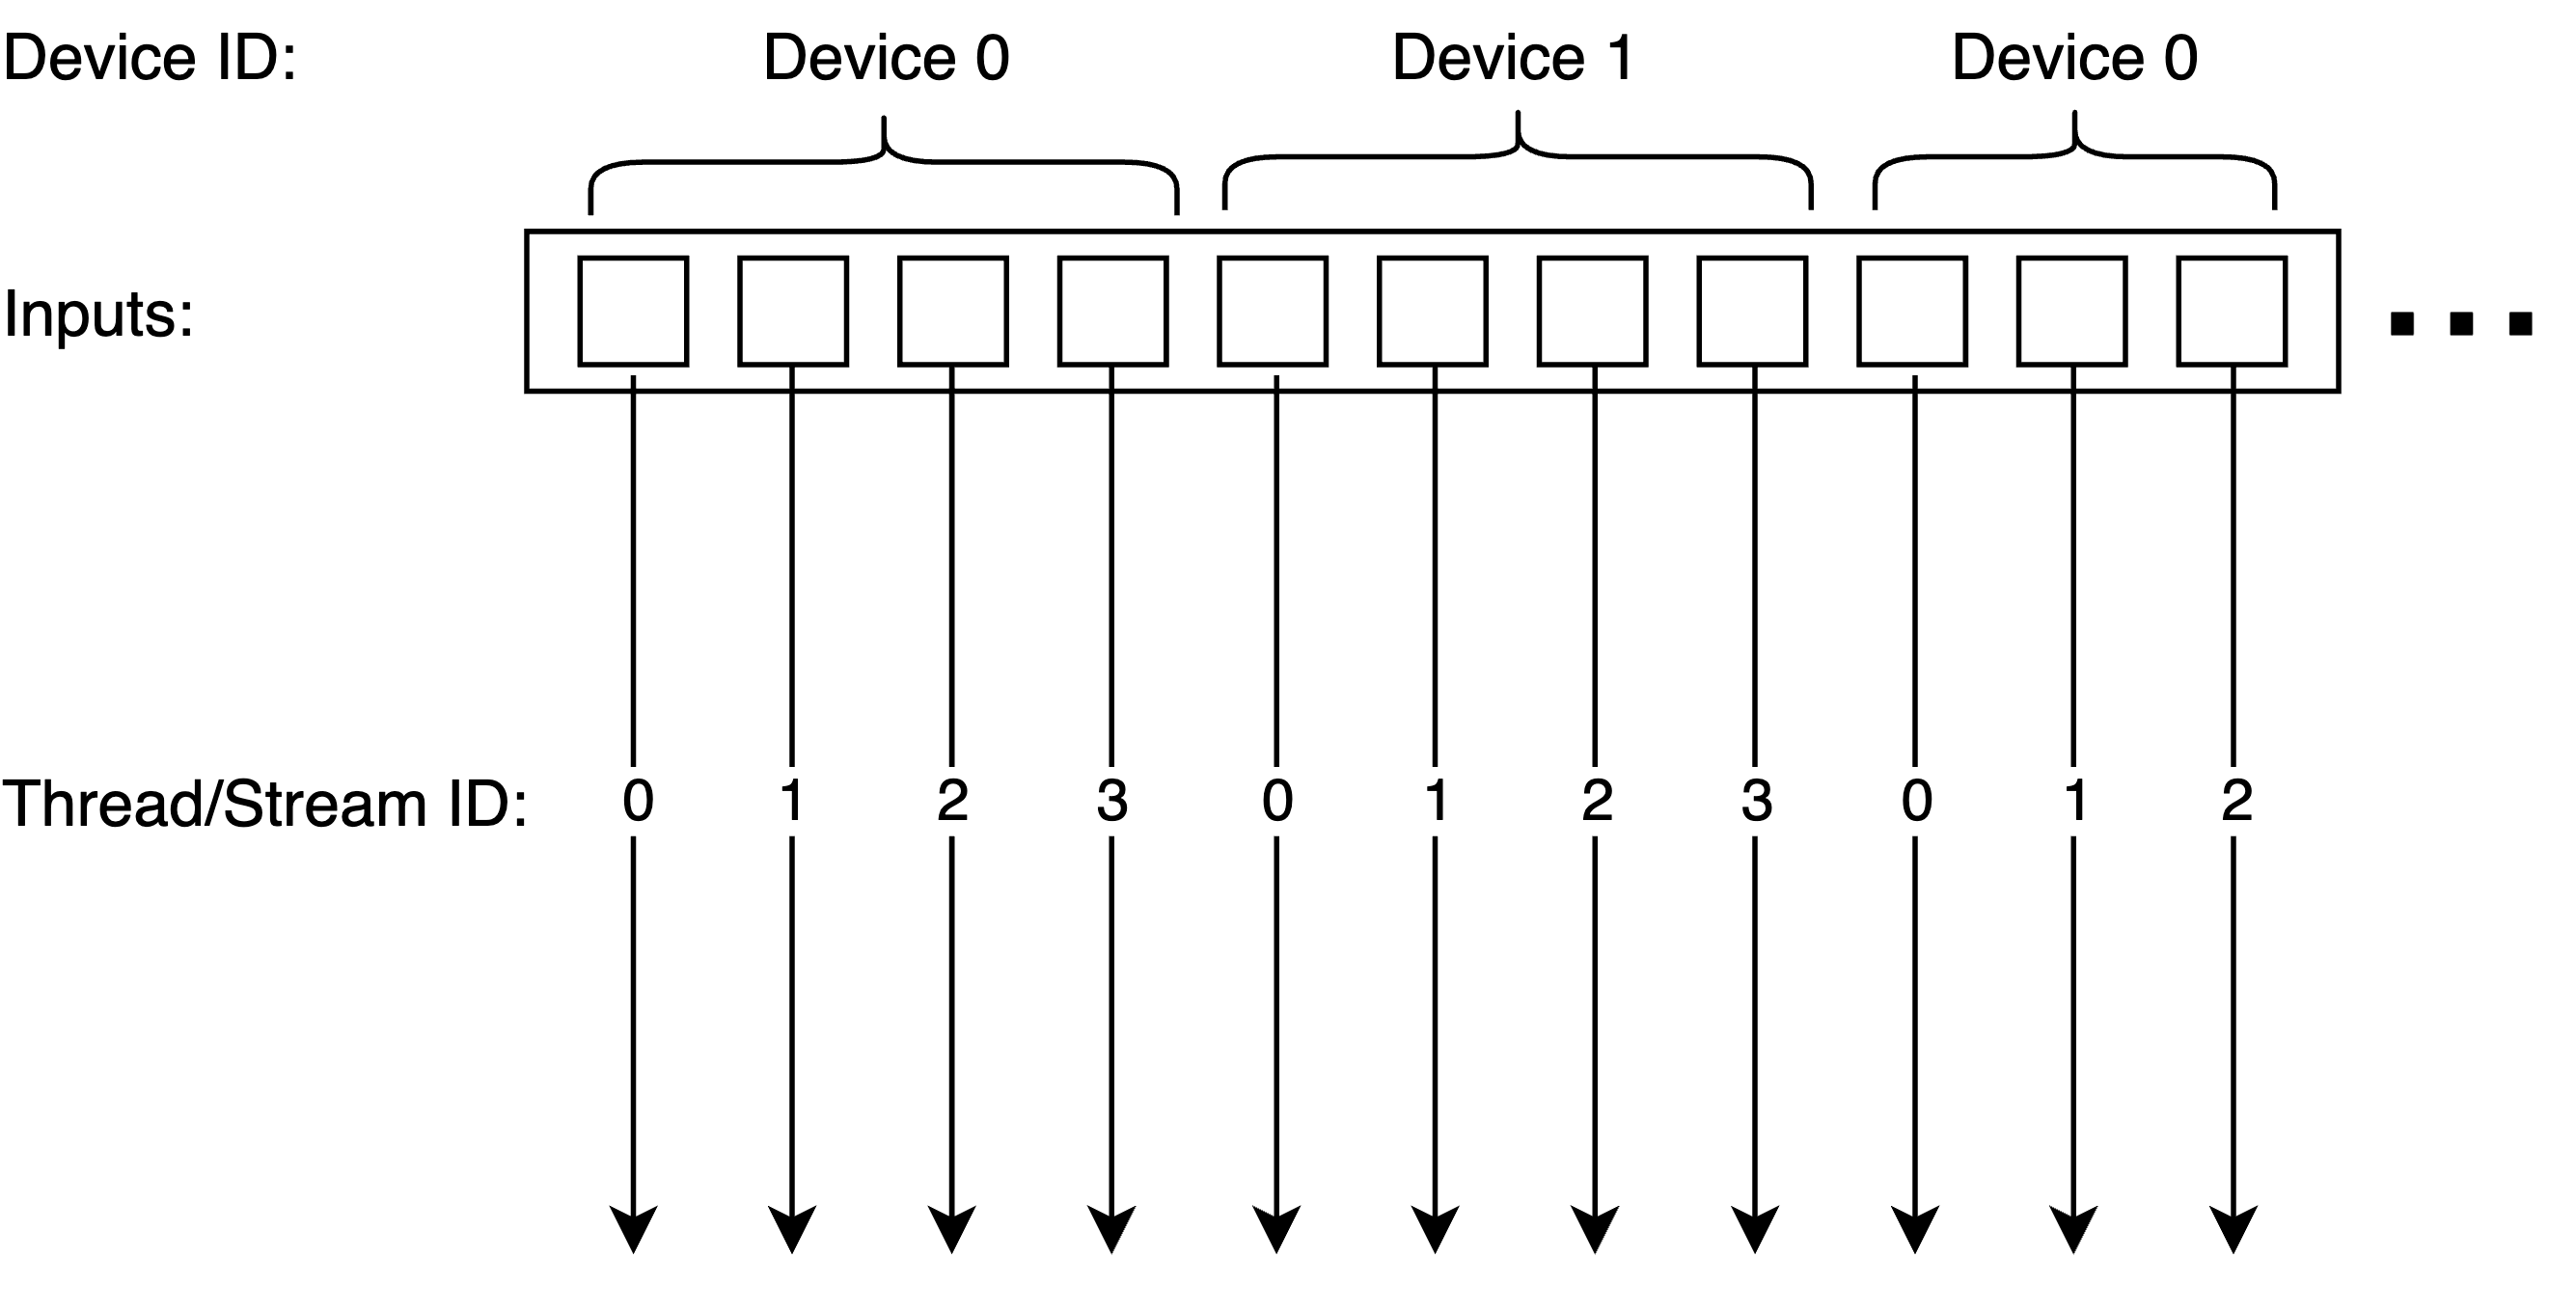
\includegraphics[width=110mm]{figures/pipeline.png}
\centering
\caption{A sample scheduling of 11 inputs to two devices with four worker threads and streams per device.}
\label{pipeline}
\end{figure}

\quad In order for this threading to be supported, the Python GIL has to be released. The data handed off to each Operation only contains the \verb|gpuarray|/\verb|gpuimage|'s encapsulated \verb|obj_data| entry which means that we do not operate on the Python object structures themselves. For every operation, the Pipeline performs a pre-processing look-up to see if the Operation is a GPU-compatible function. If so, it uses the simplified \verb|MPFunc| interface for execution so that no Python functions are called while the GIL is released. If one of the Operations does not have a corresponding \verb|MPFunc| variant, such as user-defined functions, the GIL has to be re-acquired for the duration of that Operation's execution which will impact threading performance.

\quad Individual Pipeline instances can be connected together. When this happens, the outputs of one Pipeline become the inputs to another once the first Pipeline has completed all Operations on the given input. One advantage of doing this is that separate groupings of Operations can be executed on different devices. This might be preferable for users who want a clear separation of tasks rather than wanting to bundle all Operations together. As soon as one device finishes with an input, it can hand it off to the next device and immediately begin on the next input. Millipyde will attempt to schedule both Pipelines on separate devices using the best device available. `Best' is defined the same way as previously described using the maximum metric $(mcu * mcf)$ where $mcu$ is the maximum number of compute units and $mcf$ is the maximum clock frequency. The method used for assignment is shown in Algorithm \ref{alg:pipelineDevices}


\begin{algorithm}
\caption{Decision flow for assigning devices to Pipelines i and j.}
\label{alg:pipelineDevices}
\uIf{Only one device is available}
{
    $i\gets$ only available device\;
    $j\gets$ only available device\;
}
\uElseIf{Neither $i$ nor $j$ are assigned to devices}
{
    $i\gets$ Best device available\;
    $j\gets$ Second best device available\;
}
\uElseIf{$i$ is assigned to a device and $j$ is not}
{
    $j\gets$ The best device so that $i \neq j$\;
}
\uElseIf{$j$ is assigned to a device and $i$ is not}
{
    $i\gets$ The best device so that $j \neq i$\;
}
\phantom{}
\end{algorithm}

\quad Pipelines synchronize once all Operations have been completed on all inputs which allows Python users to safely know that all work has been completed and all objects are safe to use once the \verb|run| method returns. This synchronization step also synchronizes with all other pipelines that are connected to the current Pipeline before returning. This also works for all Pipelines that are connected together if more than two Pipelines are connected to form a long chain. This same synchronization point is also when the Millipyde backend waits for all thread workers to become idle again and safely reclaims the GIL. 


\subsection{Generator Object}

Generators, like Pipelines, take a list of GPU-compatible inputs (\verb|gpuarrays| and/or \verb|gpuimages|) and perform a list of Operations on each one. Despite this, in many ways Generators are the opposite of Pipelines. Rather than mutating the input list, Generators copy each input so that the original list and list contents are left unmodified. While Pipelines have a fixed output size equal to the input size, Generators can produce any number of outputs. While Pipelines wait for all work to be completed on all inputs before synchronizing, Generators synchronize after each individual output is produced. This is because Generators are designed to produce one output as a time on-demand when the user is ready for the next one.

\quad Generators use the Python iterator protocol by including definitions for the special methods \verb|__iter__| and \verb|__next__|. The \verb|__iter__| method produces a new instance of our Generator, while \verb|__next__| produces the next output. The combination of these two methods allows Python users to iterate through the Generator in a loop to produce outputs, or to call the \verb|next()| function when an output is desired. Examples of these uses can be seen in the API in Chapter 9. When constructing a Generator, users can optionally specify an `outputs' argument for the maximum number of outputs to produce. This value can be smaller than the included number of inputs, greater than the included number of inputs, or be excluded entirely to produce infinite outputs. If the value is not infinity, a \verb|StopIteration| exception will be thrown once all outputs have been produced allowing any loop-based iteration to safely stop. 

\quad Generators also include an optional boolean parameter called \verb|return_to_host| that can be specified during construction. If this is set to \verb|True|, the Generator will turn the resulting GPU-compatible input into a NumPy \verb|ndarray| before returning it to the user. It will also free up any GPU-resources in the process. If this value is left out or set to \verb|False|, then the results produced by the Generator will be left in their \verb|gpuarray|/\verb|gpuimage| form.

\definecolor{dkgreen}{rgb}{0,0.6,0}
\definecolor{gray}{rgb}{0.5,0.5,0.5}
\definecolor{mauve}{rgb}{0.58,0,0.82}
\definecolor{backcolour}{rgb}{0.95,0.95,0.92}

\lstset{frame=none,
backgroundcolor=\color{backcolour}, 
  language=Python,
  aboveskip=5mm,
  belowskip=5mm,
  showstringspaces=false,
  columns=flexible,
  basicstyle={\linespread{0.8}\small\ttfamily},
  numbers=none,
  numberstyle=\tiny\color{gray},
  keywordstyle=\color{dkgreen},
  commentstyle=\color{blue},
  stringstyle=\color{mauve},
  breaklines=false,
  breakatwhitespace=true,
  tabsize=3
}

\chapter{Application for Image Augmentation}

\section{Image Augmentation Background}

Convolutional Neural Networks (CNNs) have quickly become a go-to solution for image classification following the popularization of deep learning \cite{dataAugment}. CNNs start with an input representation of an image such as the a 3D matrix of RGB values. With a convolution step, a tile is slid across the input and applies filters on each region to compute new features and store them in an output feature map. The CNN continues to learn by finding values for the filter matrix that can better extract useful features from the input feature map. In a pooling step, the feature map is downsampled while preserving its critical features. This means that with each new layer in the network, the dimensions of the input are reduced while expanding the depth of the feature map. The end result is one or more fully connected layers where every node in a higher level layer is connected to every node in the lower level layer. A final output function can use the final layer to compute the probability that the input image matches a given classification.

\quad One common problem with these networks, however, is overfitting. Overfitting refers to a phenomena where the model created starts to closely match the input training data. This is a problem if the input data set does not generalize well to a variety of other valid inputs. The first most obvious solution to this problem is to make sure input data sets are sufficiently large and varied. This is a problem, however, in applications such as medical imaging where there aren't enough inputs available to overcome overfitting \cite{imageAugmentationSurvey}. Data augmentation refers to another possible solution to this problem where a smaller input data set is augmented with a series of transforms and modifications to produces a larger output set \cite{dataAugment, effectivenessDataAugmentation}. 

\quad Many tools exist for this such as the Python deep learning library Keras that includes whats called an \verb|ImageDataGenerator| \cite{keras}. This class allows users to construct an object instance using a variety of parameters that are used to generate augmented output images. Using the \verb|ImageDataGenerator| class, images are produced in real-time as they are needed by the training model. Python image augmentation libraries conventionally perform the augmentation itself on the CPU while performing the learning itself on the GPU. This creates a unique opportunity to use the constructs included in Millipyde to create an on-device augmentation function similar to Keras' \verb|ImageDataGenerator|.

\section{Image Augmentation in Millipyde}

In addition to having accessible CPU counterparts for comparison, there are many other advantages to experimenting with image augmentation in Millipyde. Since image augmentation is based on image transformations, it is ripe for GPU accelerations, and it can leverage Millipyde's builtin \verb|gpuimage| methods. The results were also easy to verify. Initial implementations used probabilities of 1 for guaranteed function execution as well as single-point ranges for each random image transformations. Millipyde's testing scripts could then verify with pixel-level accuracy that each image matched the expected output. The probability could gradually be lowered in addition to introducing larger random ranges to introduce higher degrees of variability into the results. Each \verb|gpuimage| can be manually inspected for verification, and multiple were used to confirm that there was a degree of random variation. 

\quad As shown in the sample code in Figure \ref{augmentCode}, the Millipyde code can closely mirror the behavior of other image augmentation libraries. By choosing the Generator rather than the Pipeline, results can be produced on the fly as they are needed by a future training model. The Generator's copy semantics also lets us produce an output set that is larger than the original input set. For the purpose of this demonstration, the \verb|return_to_host| flag was set to true and the images were saved as output files that can be viewed and studied. In practice, it may be desirable to avoid saving the images entirely and to keep their memory contents on-device so that it can be used by the learning-phase. This demo resulted in 48 new images created from an input size of 6 images as shown in Figure \ref{augmentResults}. 

\begin{figure}
\begin{lstlisting}
from skimage.io import imsave

import millipyde as mp

def augment():
    images = mp.images_from_path("examples/augment_in")

    ops = [
        mp.Operation("transpose", probability=.2),
        mp.Operation("fliplr", probability=.2),
        mp.Operation("random_brightness", -.2, 1),
        mp.Operation("random_gaussian", 0, 2),
        mp.Operation("random_colorize", [.5, 1.5], [.5, 1.5], [.5, 1.5], 
                probability=.3),
        mp.Operation("rgb2grey", probability=.3),
        mp.Operation("random_rotate", 0, 120, probability = .5)
    ]

    g = mp.Generator(images, ops, return_to_host=True)

    for i in range(48):
        img = next(g)
        imsave("examples/augment_out/dog" + str(i) + ".png", img)
    
def main():
    augment()

if __name__ == '__main__':
    main()
\end{lstlisting}
\caption{The Python code used to augment images using Millipyde.}
\label{augmentCode}
\end{figure}

\begin{figure}[hbtp]
\includegraphics[width=\textwidth]{figures/AugmentationResults.png}
\centering
\caption{Augmenting six input images to produce 48 output images}
\label{augmentResults}
\end{figure}

\section{Results Discussion}

Each column in Figure \ref{augmentResults} represents an augmentation of one of the same six original input images. As seen in the diversity across each row, our implementation succeeded in producing a wide variety of results. No two images ended up quite the same, but each output could be used as an example of a dog for a future training algorithm. In some cases, the transformations might be too extreme to work optimally for image classification applications, so the parameters and probabilities can be further tuned by users in this field. The dog in the first image, for example, loses some of its edges to the background with the combination of random transformations selected. We look forward to testing Millipyde augmentation in-depth with future practical computer vision applications.
\definecolor{dkgreen}{rgb}{0,0.6,0}
\definecolor{gray}{rgb}{0.5,0.5,0.5}
\definecolor{mauve}{rgb}{0.58,0,0.82}

\lstset{frame=none,
  language=Python,
  aboveskip=5mm,
  belowskip=5mm,
  showstringspaces=false,
  columns=flexible,
  basicstyle={\linespread{0.8}\small\ttfamily},
  numbers=none,
  numberstyle=\tiny\color{gray},
  keywordstyle=\color{dkgreen},
  commentstyle=\color{blue},
  stringstyle=\color{mauve},
  breaklines=false,
  breakatwhitespace=true,
  tabsize=3
}

\chapter{Evaluation}

\section{Test and Development Environment}

Millipyde was tested using a desktop workstation with the following specifications: 
\begin{itemize}
  \item Intel Xeon CPU E5-1620 @ 3.50GHz
  \item 32 GB memory
  \item Ubuntu 20.04.3 LTS Operating System
\end{itemize}

The workstation was equipped with two of the following GPU:
\begin{itemize}
  \item AMD Vega 10 XTX (gfx900) GPU
  \item Wavefront size: 64
  \item 64 CUs with 4 SIMDs per CU
  \item 4 Shader Engines
  \item 16KB L1 cache, 4096KB L2 cache
\end{itemize}

\quad Using the system BIOS, the workstation was configured to use large-BAR configuration to expose GPU local memory via PCIe memory BARs. This increased the BAR size to 64 bits, and was required to allow Millipyde to use DMA peer-to-peer memory transfers for any experiments that used both GPUs \cite{rocmrdma}. 

\section{Single Function Benchmarks}

To test performance with individual functions, we used select Millipyde functions that had functionally-equivalent implementations in the non-GPU accelerated library scikit-image. These functions were run on identical images, and their performance was measured using Python's \verb|time.perf_counter| function. This measurement only included the time for the function itself to execute. It excludes the time for the image to be opened and saved. To ensure accuracy and consistency across both implementations, very pixel value in both the scikit-image output and the Millipyde output were compared to 4 decimal places. These benchmark were run on 12 copies of the same image in different sizes. They start at 500 pixels wide and go up to 6000 pixels wide, stepping by 500 pixels every time. 

\subsection{Gamma Correction}

One of the most basic categories of parallel computations are element-wise calculations where each data value in an array undergoes a standalone operation to compute the respective output data value in the resulting array. One such example is Millipyde's \verb|adjust_gamma| function. Each pixel is transformed using the equation $V_{out} = A * V_{in} ^ \gamma$ where  $A$ is a constant multiplier called `gain', and $\gamma$ is the gamma adjustment value. This results in a brightness correction where gamma values less than one increase the overall brightness, and values greater than one decrease the brightness. The effects of this can be seen in Figure \ref{gammaExample}. For our experiments, we ran both the Millipyde function and the scikit-image equivalent with a gamma of 2 and gain of 1.

\begin{figure}[H]
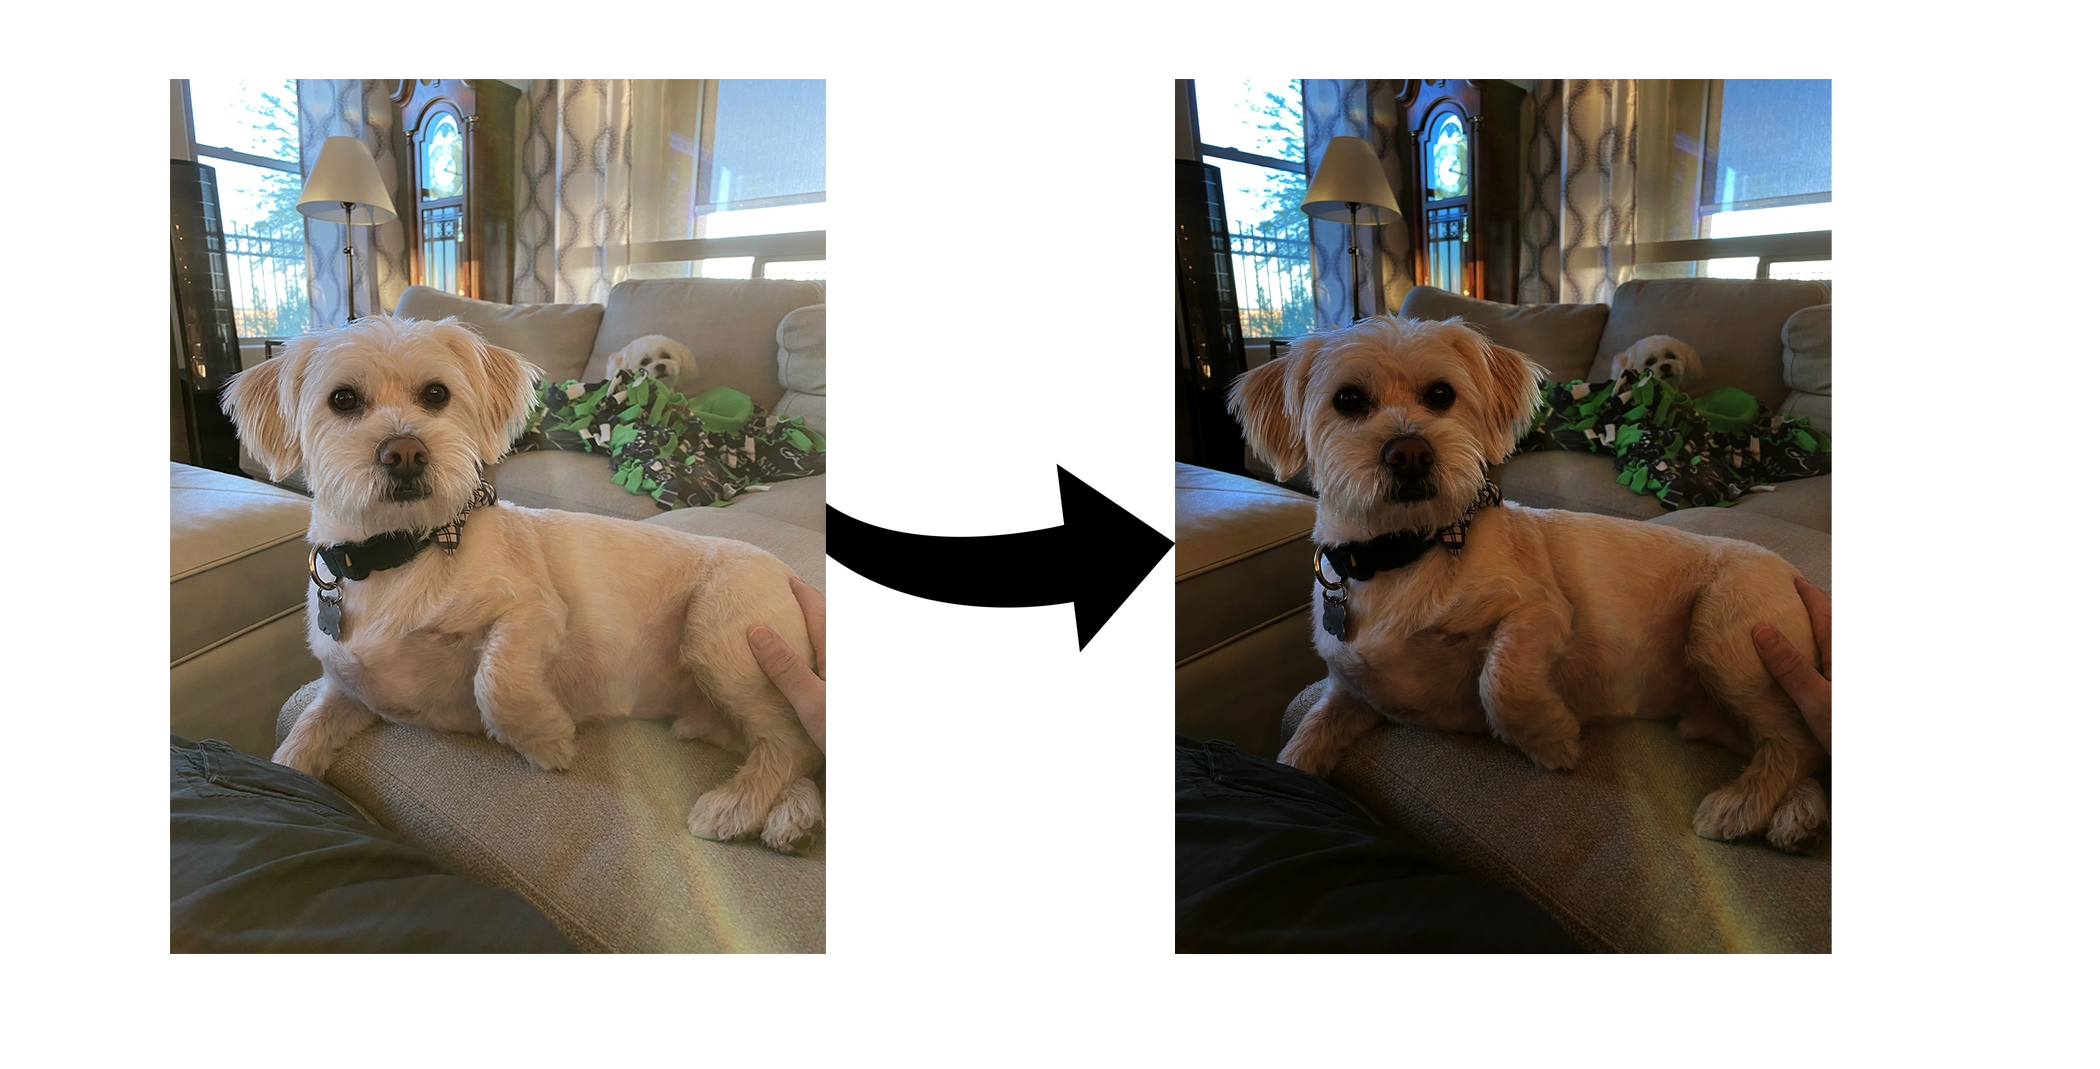
\includegraphics[width=\textwidth]{figures/GammaExample.png}
\centering
\caption{The effects of gamma correction using a gamma value of 2.}
\label{gammaExample}
\end{figure}

\begin{table}[h!]
\centering
\begin{tabular}{ |c|c|c|c| } 
\hline
image size & scikit-image time (s) & Millipyde time (s) & \% difference \\
\hline
500&0.0030651&0.0001561&1964 \\
1000&0.0105069&0.0001869&5622 \\
1500&0.0262136&0.0002929&8950 \\
2000&0.0403756&0.0004912&8220 \\ 
2500&0.0624683&0.0006293&9927 \\
3000&0.0890932&0.0009215&9668 \\
3500&0.1531737&0.0011845&12932 \\
4000&0.1878477&0.0015242&12324 \\
4500&0.2309318&0.0018687&12358 \\ 
5000&0.2741731&0.0022279&12306 \\
5500&0.3252361&0.0027007&12043 \\
6000&0.3819223&0.0031833&11998 \\
\hline
\end{tabular}
\caption{Timing results for gamma correction using scikit-image and Millipyde.}
\label{gammaTable}
\end{table}

\begin{figure}[H]
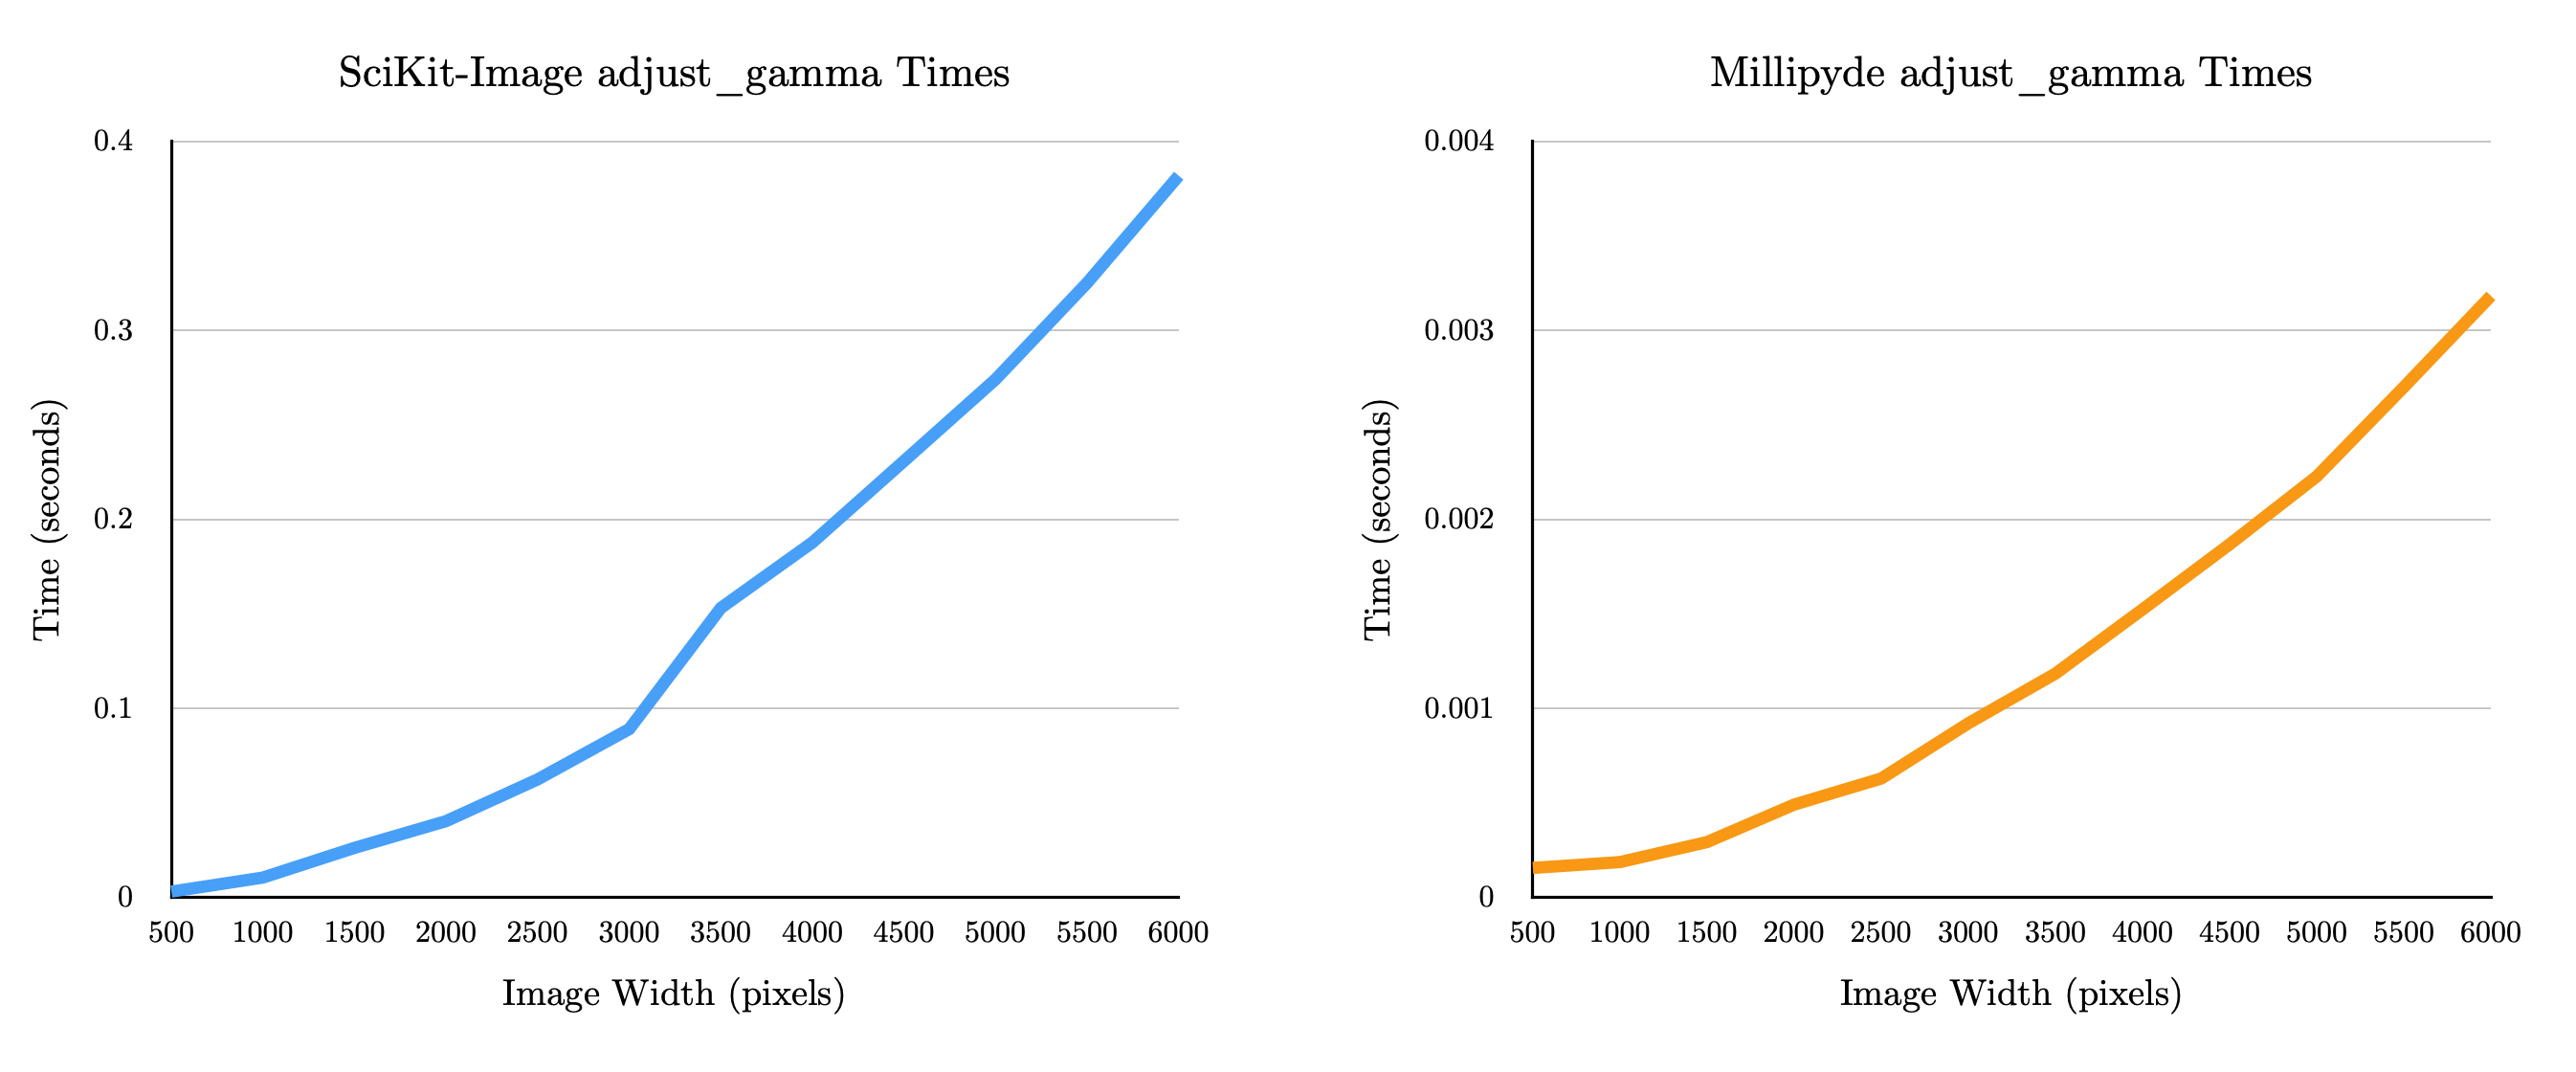
\includegraphics[width=\textwidth]{figures/GammaComparison.png}
\centering
\caption{Graphical representation of the time spent performing gamma correction on an image in scikit-image compared to its GPU-accelerated equivalent in Millipyde.}
\label{gammaComparison}
\end{figure}

\quad The results demonstrated a predictable decrease in runtime for the GPU-accelerated function. It ranged from around 20x faster for the 500-pixel image to more than 100x faster for larger images. These results when graphed followed a clean curve that closely mirrored the scikit-image equivalent as shown in Table \ref{gammaTable} and Figure \ref{gammaComparison}. Users can reliably expect the Millipyde gamma correction functionality to be faster than CPU-only equivalent functions.

\subsection{Greyscale}

 A slightly more complicated variation on a element-wise kernels happens when the dimensions of the input array are different than that of the output array. This can be seen in greyscale conversion functions which translates from a 3-dimensional RGB array of 8-bit integer values to a 2-dimensional array of floating point values. This computation is traditionally done using a weighted sum of the RGB components in an image to produce a single greyscale value between 1 and 0. Both Millipyde and scikit-image use the following weights in this calculation: $Y = 0.2125 R + 0.7154 G + 0.0721 B$ \cite{skirgb2grey}. 
This makes it a good function to use in comparing scikit-image's functionality with the GPU-parallelized implementation in Millipyde. 

\begin{figure}[hbtp]
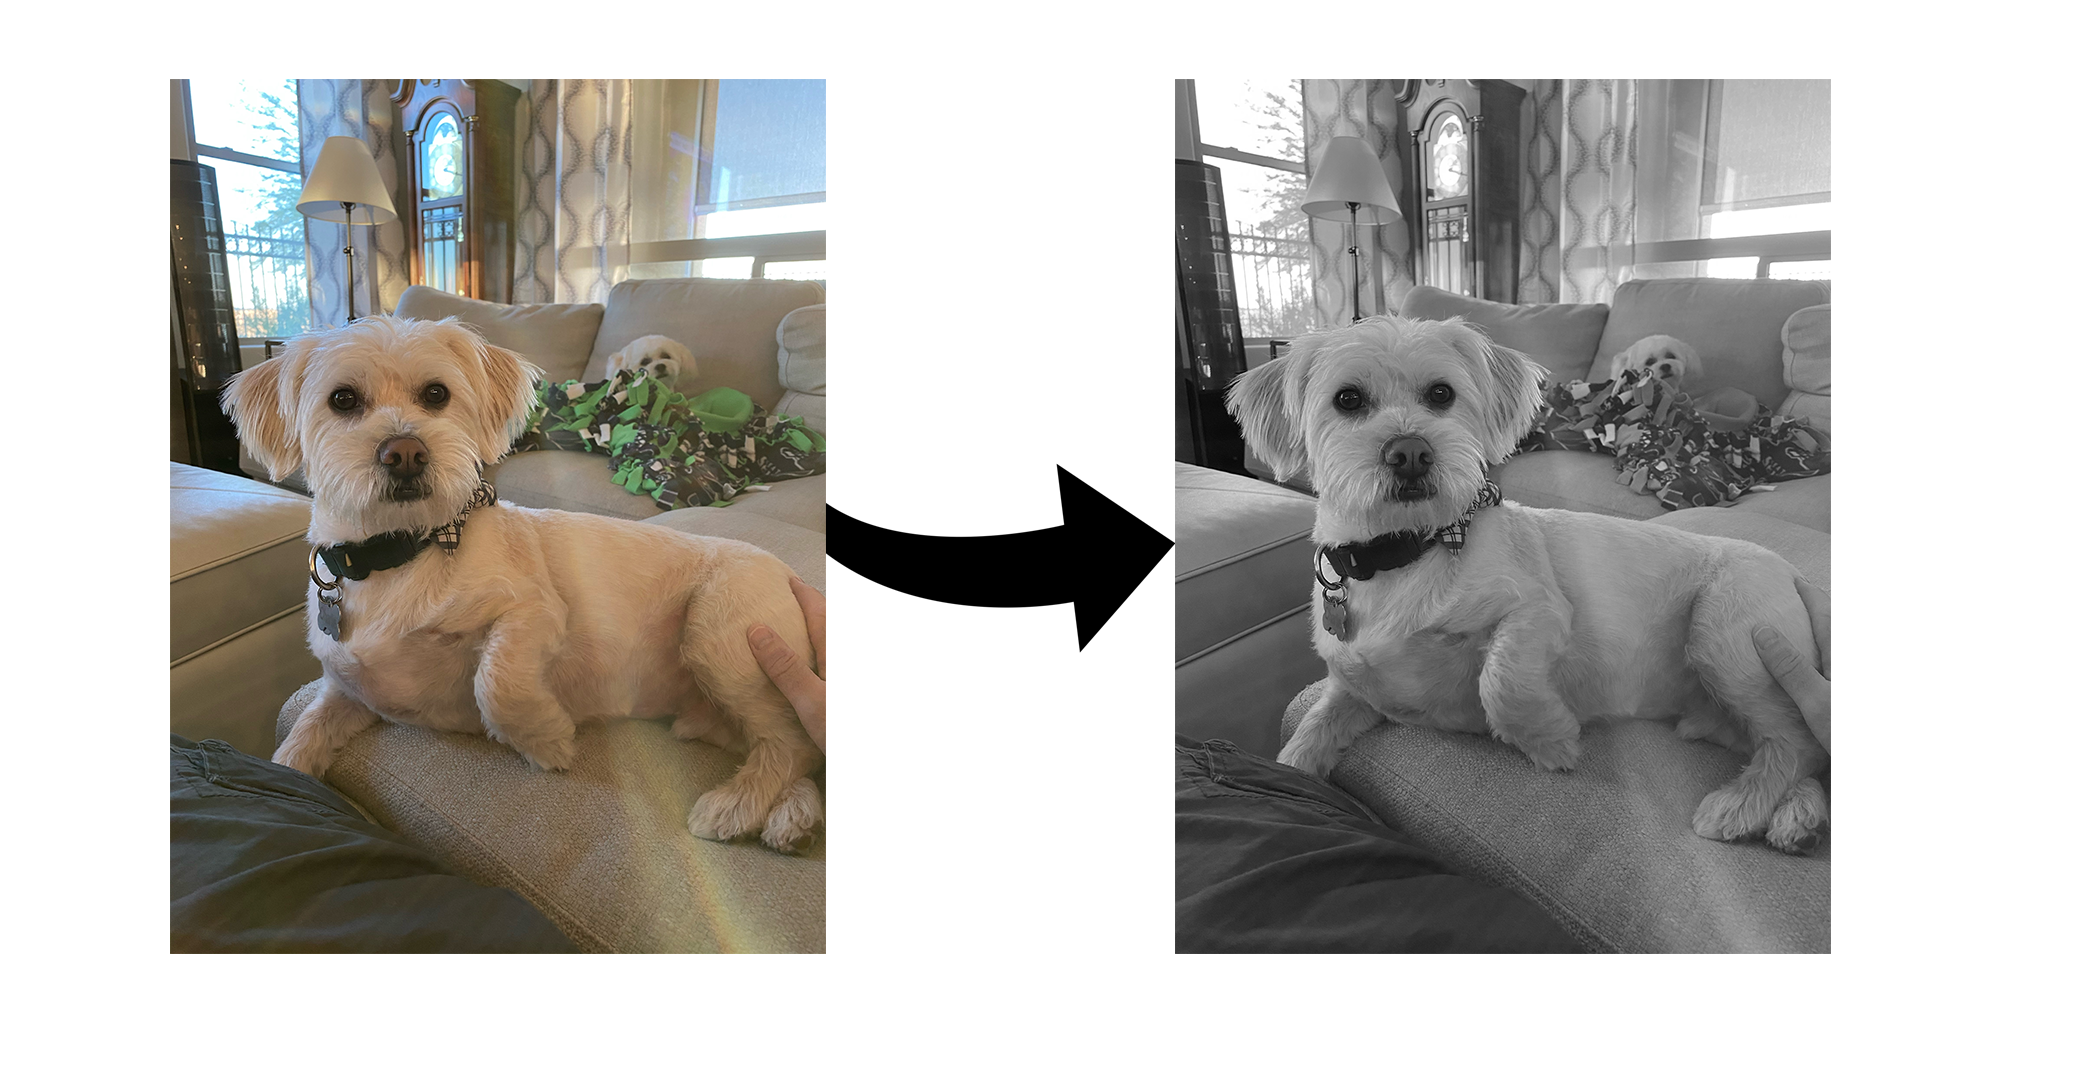
\includegraphics[width=\textwidth]{figures/GreyscaleExample.png}
\centering
\caption{The effects of greyscaling an RGB image.}
\label{greyscaleExample}
\end{figure}

\begin{table}[H]
\centering
\begin{tabular}{ |c|c|c|c| } 
\hline
image size & scikit-image time (s) & Millipyde time (s) & \% difference \\
\hline
500 & 0.0063839 & 0.0014073 & 454 \\
1000 & 0.0260336&0.0014537&1790 \\
1500&0.0535500&0.0052456&1021 \\
2000&0.0942788&0.0055702&1693 \\
2500&0.1466724&0.0054552&2689 \\
3000&0.2102404&0.0065436&3213 \\ 
3500&0.2964064&0.0091423&3242 \\
4000&0.3863234&0.0085288&4530 \\
4500&0.4974762&0.0089737&5544 \\
5000&0.6113694&0.0092912&6580 \\
5500&0.7201406&0.0092047&7824 \\
6000&0.8563366&0.0115259&7516 \\
\hline
\end{tabular}
\caption{Timing results for greyscaling images using scikit-image and Millipyde.}
\label{greyscaleTable}
\end{table}

\begin{figure}[H]
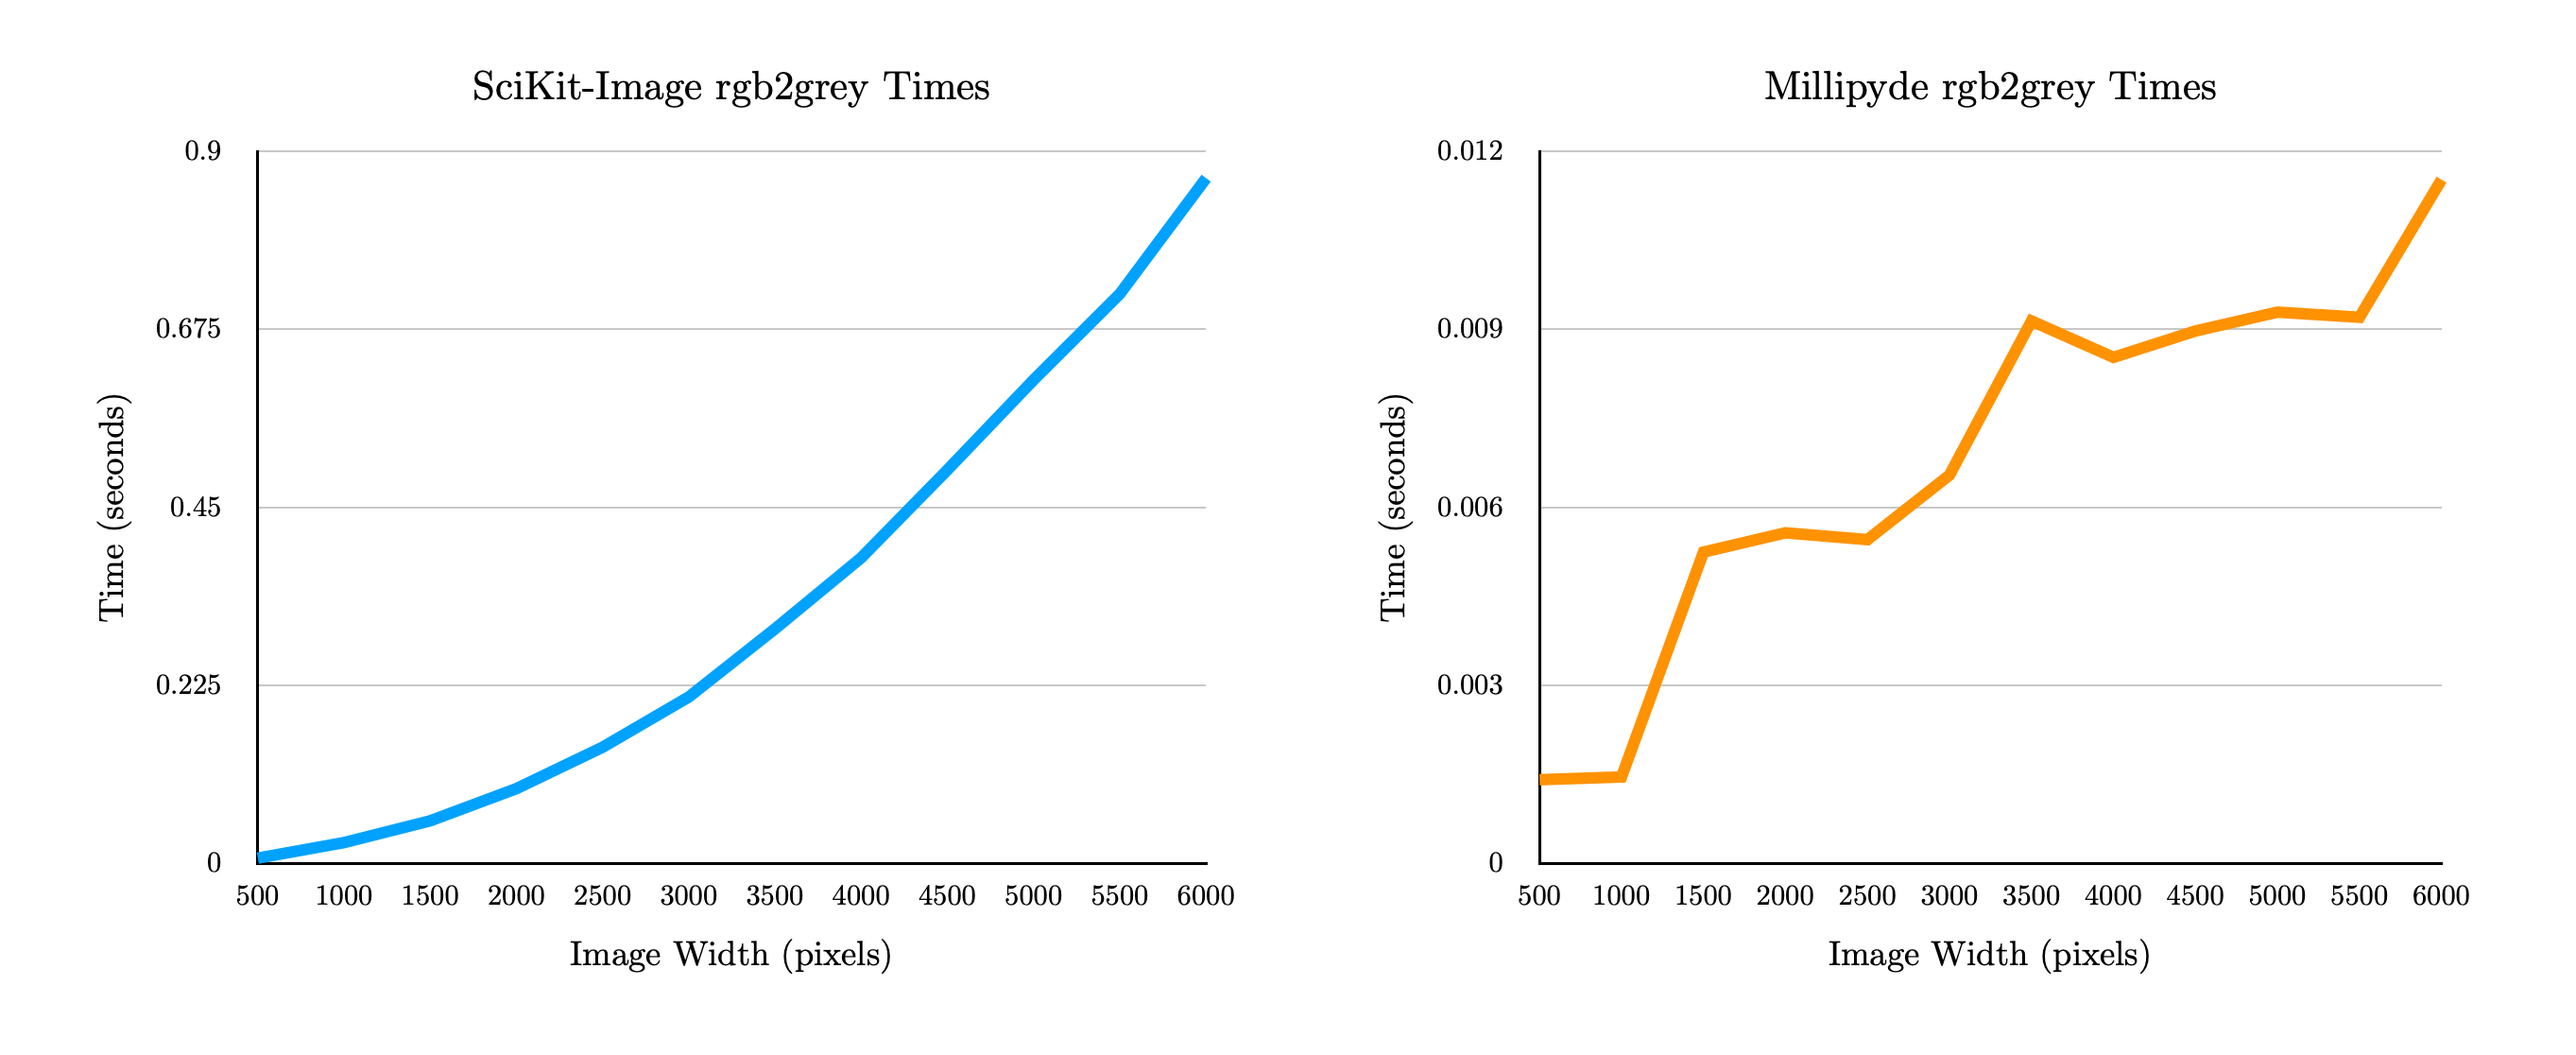
\includegraphics[width=\textwidth]{figures/greyscaleComparison.png}
\centering
\caption{Graphical representation of the time spent greyscaling an image in scikit-image compared to its GPU-accelerated equivalent in Millipyde.}
\label{greyscaleComparison}
\end{figure}

\quad As shown in Table \ref{greyscaleTable} and Figure \ref{greyscaleComparison}, these results differed surprisingly from those of the gamma correction function. On the surface, the kernels for both functions look startlingly similar -- both only perform a single element-wise computation on each input pixel. This difference in performance is therefore likely to do with the difference in shape between the input and output arrays. The resulting Millipyde graph almost resembles stair steps with significant jumps in performance between some image sizes, and stagnated performance between others. We were unable to find a clear cause based on studying the profile results of the function's runtime using the ROCm profiler 'rocprof'. Future experimentation is needed to understand this behavior, and to see if better/more predictable performance is possible. 

\subsection{Gaussian Blur Convolution}

Another large category of parallel computation is the convolution, often referred to as the stencil computation, with applications ranging from signal processing, image processing, video processing, and more \cite{greenBook}. It involves a more mathematically-complex array computation where each output element is a weighted sum of N number of neighboring elements. The weights come from an input mask array called the kernel. For this example, we will use a Gaussian blur convolution which is commonly used in image processing and computer vision for applications such as edge detection \cite{gaussEdge}. For this computation, the kernel can be modeled as a 2D convolution using the kernel $G(x, y) = \frac{1}{2 \pi \sigma^2} e^{-\frac{x^2 + y^2}{2 \sigma^2}}$ where $\sigma$ represents standard deviation. This results in a symmetric kernel with stronger weights in the middle. The Gaussian blur is also separable, meaning the same result can be achieved by a separate pass of a 1-dimensional Gaussian kernel on each axis. The calculation for the 1-dimensional kernel is $G(x) = \frac{1}{\sqrt{2 \pi \sigma^2}} e^{-\frac{x^2}{2 \sigma^2}}$.

\begin{figure}[H]
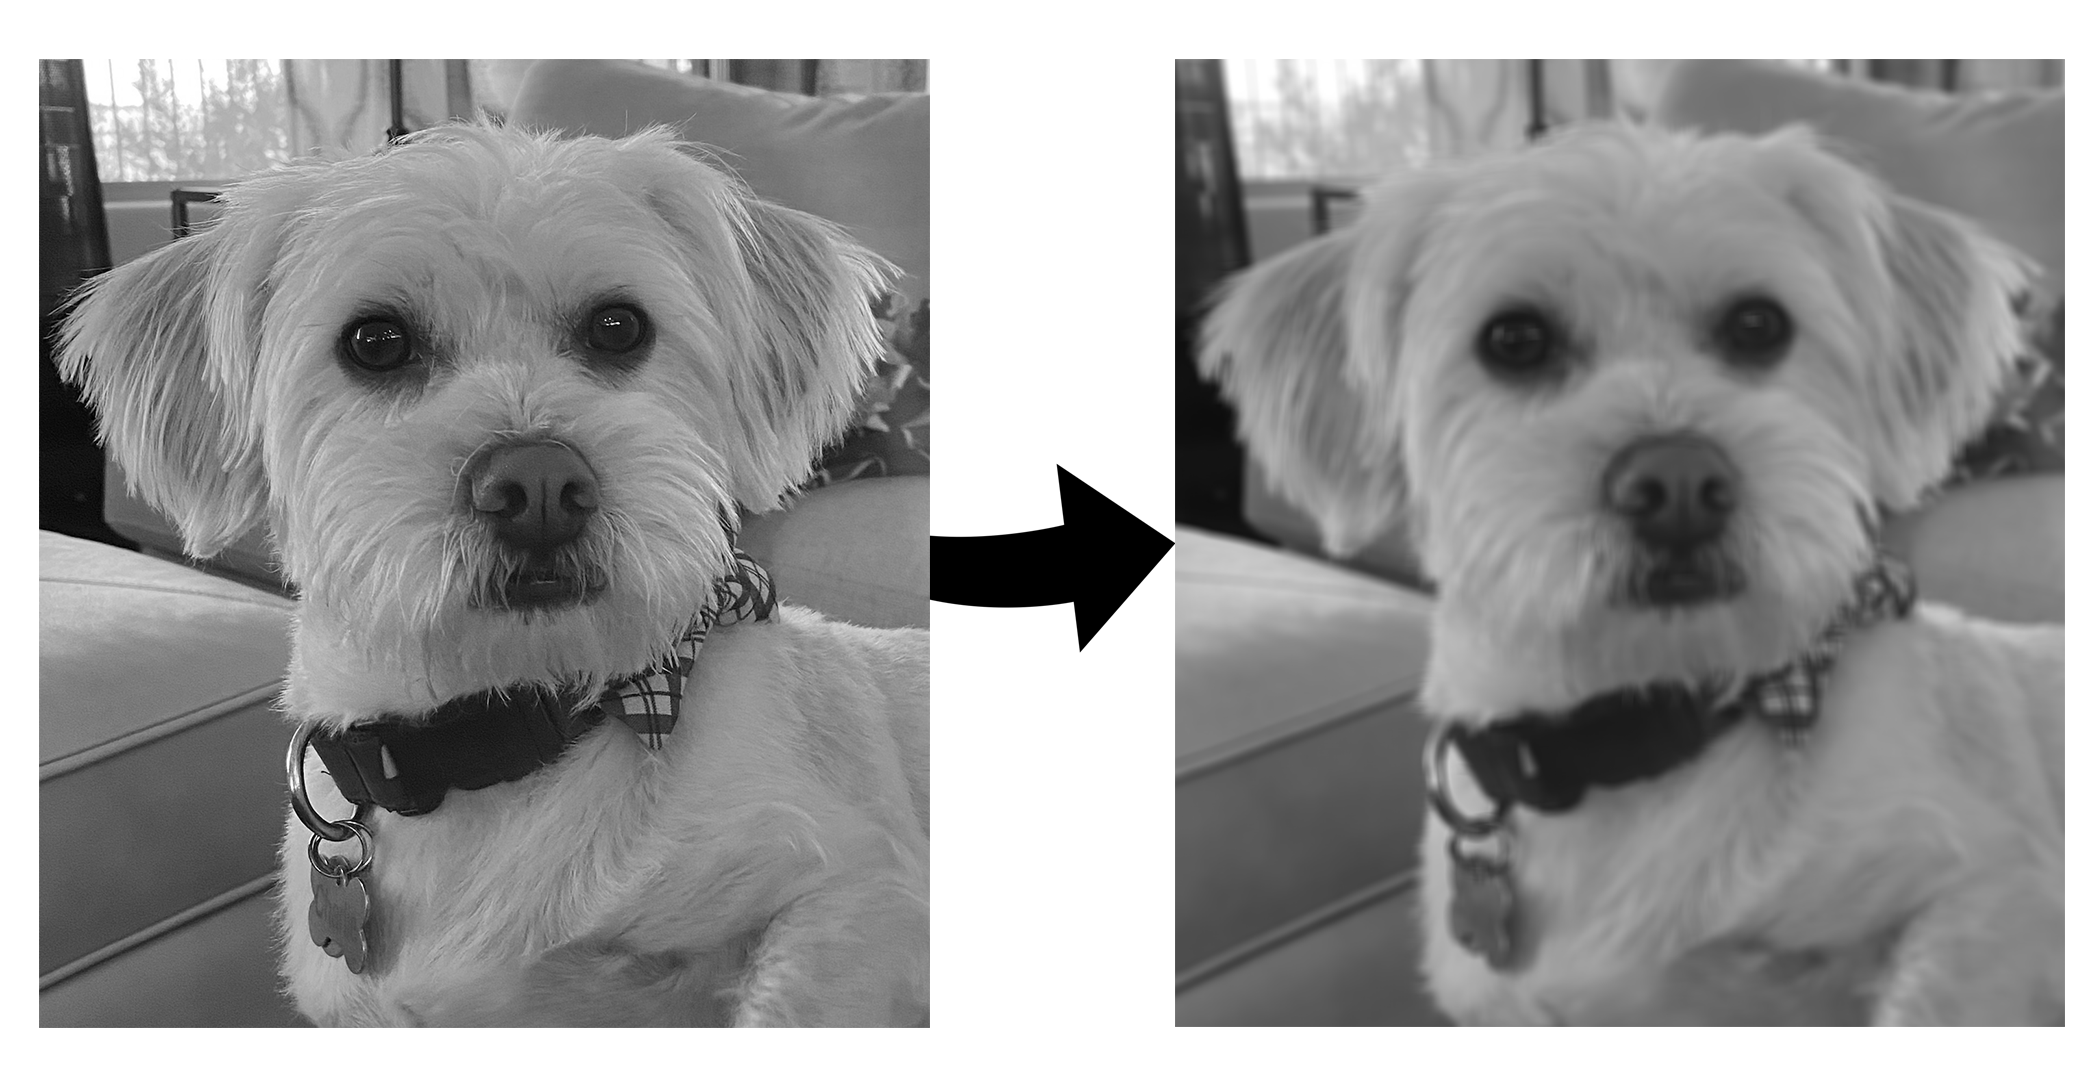
\includegraphics[width=100mm]{figures/GaussianExample2.png}
\centering
\caption{The effects of a Gaussian Blur.}
\label{augmentExample}
\end{figure}

\quad Both Millipyde and scikit-image's gaussian functions use two passes of a 1-dimensional Gaussian kernel which makes it a great example for comparison \cite{scipyGaussianSrc}. Millipyde also exploits the shared memory system on the GPU for the Gaussian function. A block of the input image is first loaded into shared memory so that each thread block has access to these pixel values. This technique was previously studied in CUDA, and it was shown to produce excellent results for GPU runtime \cite{cudaConvolution}. For this test, we used a sigma value of 2 for both Millipyde and scikit-image's benchmarks. To match the way Millipyde handle's pixel edge values and kernel widths, the following parameters were used for the scikit-image comparison:
\verb|cval=0|, \verb|truncate=8|, \verb|mode="constant"|. This ensures equal kernel sizes, and caps pixels outside of the image to a value of 0.


\begin{table}[H]
\centering
\begin{tabular}{ |c|c|c|c| } 
\hline
image size & scikit-image time (s) & Millipyde time (s) & \% difference \\
\hline
500&0.0105292&0.0002608&4037 \\
1000&0.0408449&0.0004123&9907 \\
1500&0.0902537&0.0006834&13207 \\
2000&0.1697805&0.0010704&15861 \\
2500&0.2523343&0.0015845&15925 \\
3000&0.3749286&0.0022314&16802 \\
3500&0.5563606&0.0029901&18607 \\
4000&0.7121980&0.0037107&19193 \\
4500&0.8735706&0.0047103&18546 \\
5000&1.0703184&0.0058559&18278 \\
5500&1.2964685&0.0069618&18623 \\
6000&1.5977196&0.0082425&19384 \\
\hline
\end{tabular}
\caption{Timing results for Gaussian blur using scikit-image and Millipyde.}
\label{gaussianTable}
\end{table}

\begin{figure}[H]
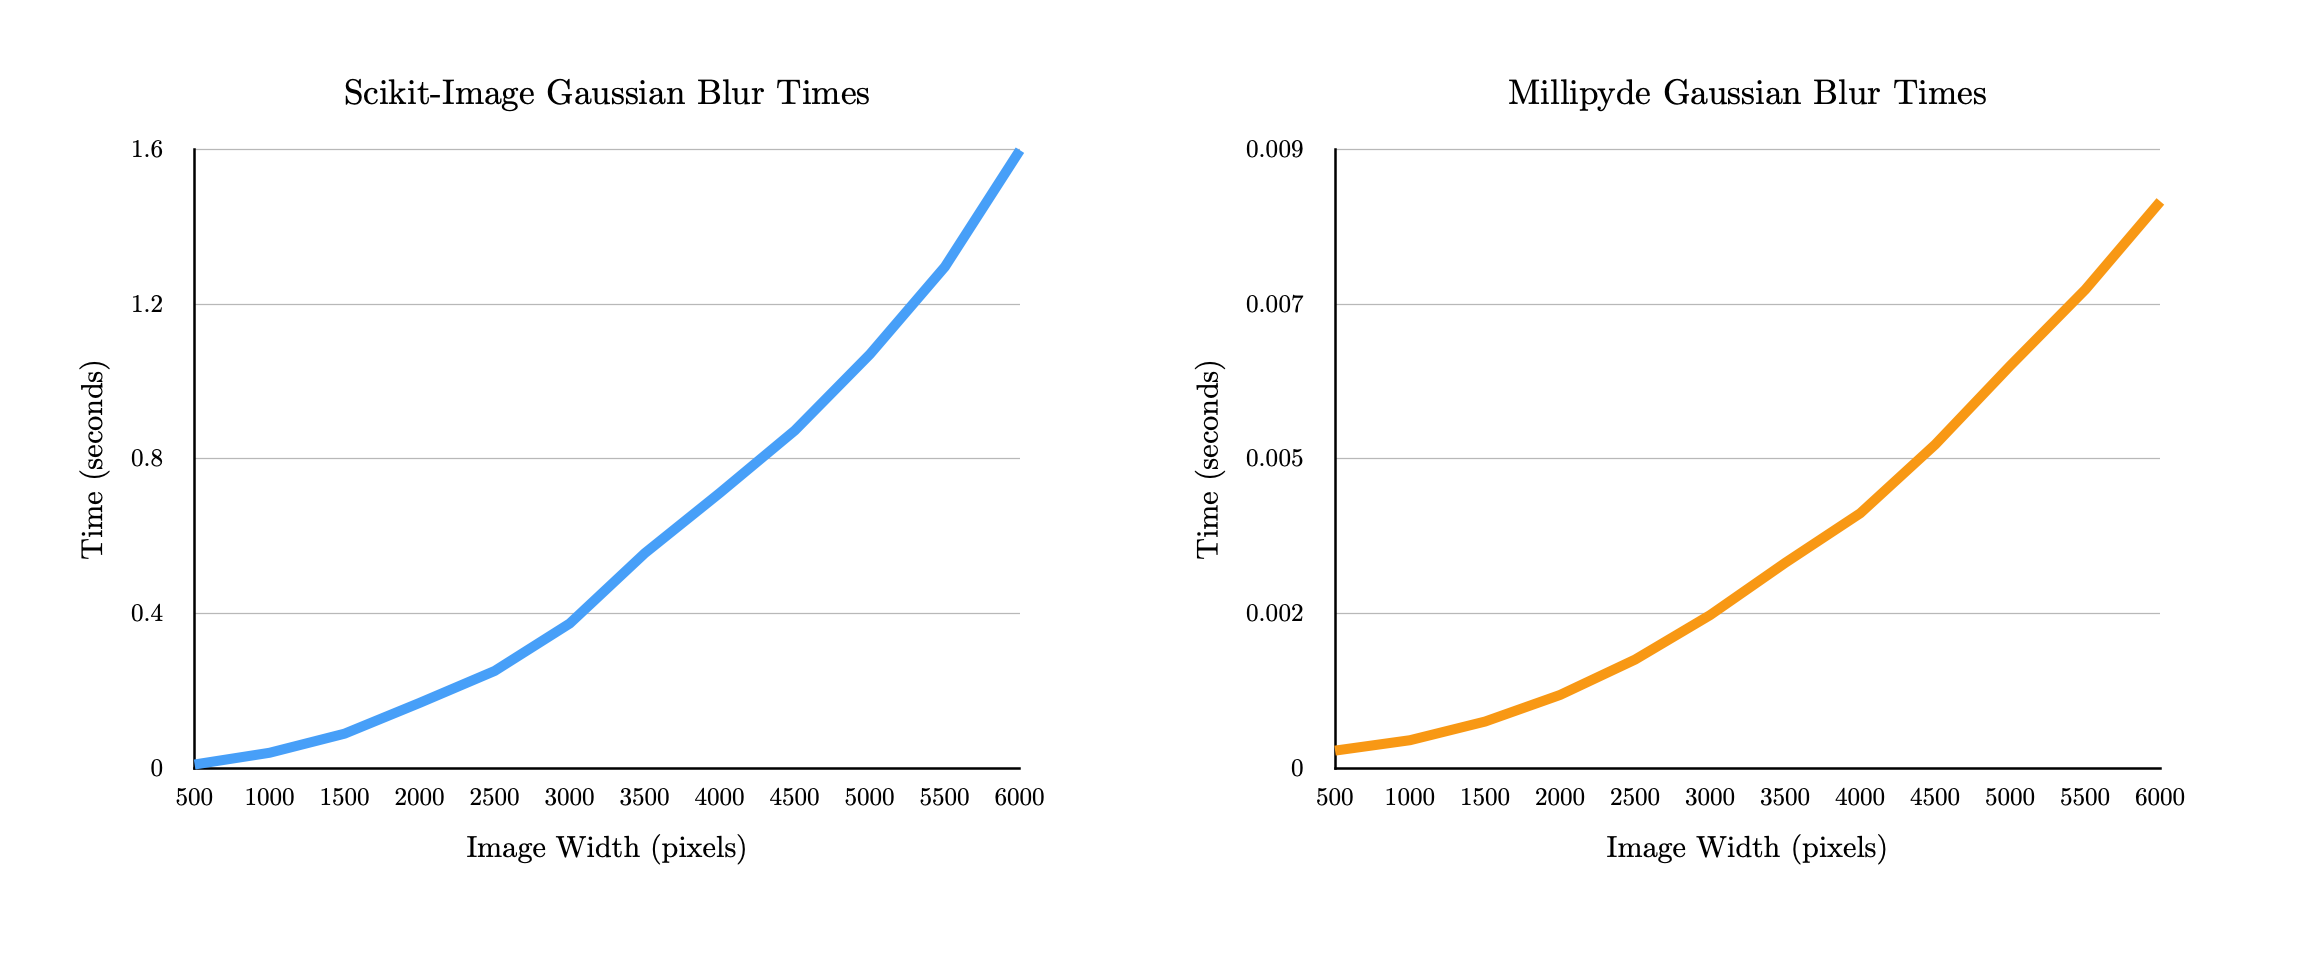
\includegraphics[width=\textwidth]{figures/gaussianComparison.png}
\centering
\caption{Graphical representation of the time spent performing a Gaussian blur on an image in scikit-image compared to its GPU-accelerated equivalent in Millipyde.}
\label{gaussianComparison}
\end{figure}

\quad This algorithm proved to be incredibly efficient in our Millipyde environment. As shown in Table \ref{gaussianTable} and Figure \ref{gaussianComparison}, our performance ranged from around 40x faster for smaller images up to just under 200x faster in larger images. Much of this performance increase is thanks to the shared memory blocks whose access times were much faster than always reading from global memory. This shows a lot of promise for future convolutional functions in Millipyde, and more experimentation should be done on utilizing shared memory in other image algorithms. 

\section{Pipeline Benchmarks}

Since our Pipeline objects exploit multiple forms of parallelism, it is worth studying the performance of various Pipeline configurations. Four our tests, we bench-marked the Pipelines using multiple copies of the same image for our list of inputs. Each image was 3500 pixels wide by 4666 pixels tall. The input list sizes ranged from 1 to 100. From there, four different configurations were run on each group of inputs. The first configuration, labeled `Control' in each respective chart, executed every Operation sequentially in a Python loop rather than using a Pipeline object at all. The test labeled `Single GPU' ran a single Pipeline that was bound to one given device so that it would not use all GPUs available on the system. The 3rd test, labeled `Dual GPUs' was not bound to a single device, so it was allowed to use both available devices for scheduling. The final test, labeled `Connected GPUs' split the work in half so that each of two Pipeline objects had half of the Operations to be completed. These two Pipelines were each bound to separate devices in the system and connected so that the outputs that completed on the first Pipeline would be transferred over to the second Pipeline to complete the remainder of the Operations.

\subsection{Pipelines with 5 Operations}

Our first experiment represented a standard small set of operations that may occur in a variety of data manipulation programs. Each iteration of the experiment used a total of five image transformation Operations. These included a Gaussian blur, gamma adjustment, horizontal flip, 45-degree rotation, and a greyscale conversion. For the connected Pipeline, these Operations were split in half so that the Gaussian blur, gamma adjustment, and flip were performed inside of the first Pipeline, and the rotation and greyscale conversion were performed on the second Pipeline.

\begin{table}[H]
\centering
\begin{tabular}{ |c|c|c|c|c| } 
\hline
Number of inputs & Control & Single GPU & Dual GPUs & Connected GPUs \\
\hline
1&	0.0244971&	0.0269347&	0.2622321&	0.0357248 \\
5&	0.1214234&	0.1228287&	0.1046105&	0.1197764\\
10&	0.2419561&	0.2456722&	0.1764512&	0.2654271\\
20&	0.4817377&	0.4817598&	0.3661450&	0.4735247\\
50&	1.2170164&	1.3320313&	0.8369642&	1.1232160\\
75&	1.9473421&	2.1429327&	1.2548219&	1.8599911\\
100&	2.9957998&	2.9042716&	1.6321600&	2.5250520\\
\hline
\end{tabular}
\caption{Timing results for running a short 5-Operation pipeline}
\label{pipelineTable1}
\end{table}

\begin{figure}[H]
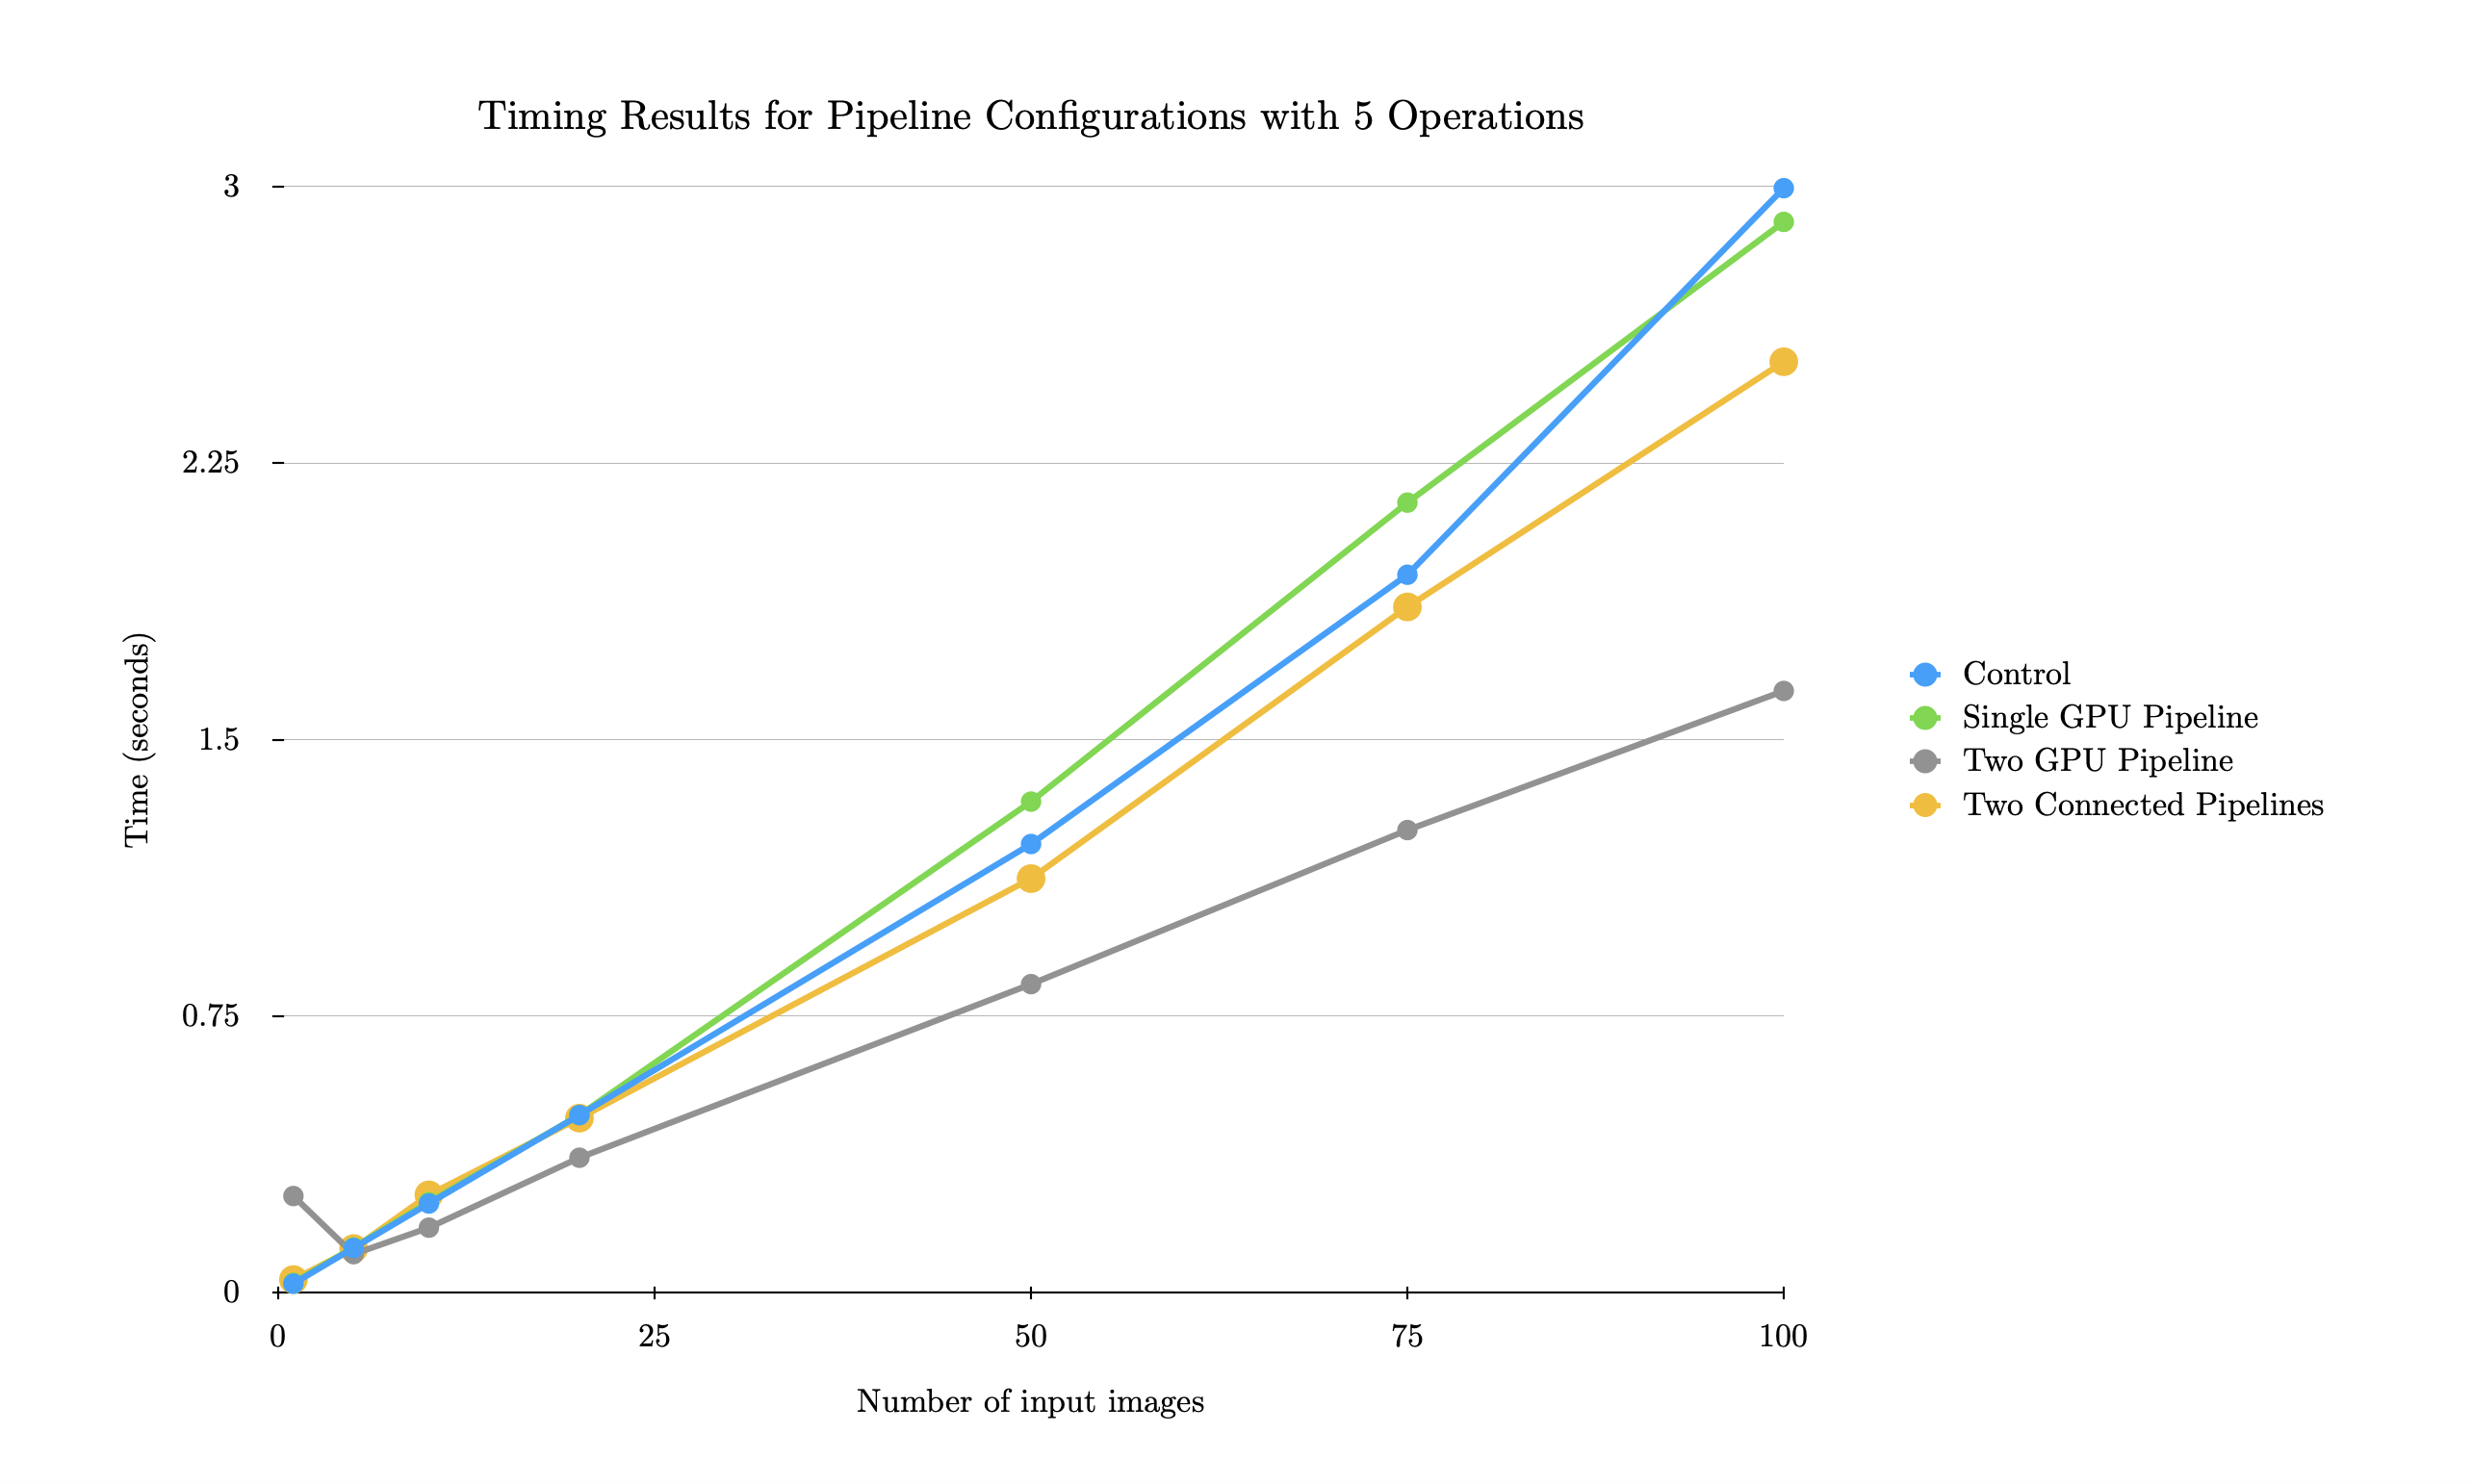
\includegraphics[width=\textwidth]{figures/pipelineChart1.png}
\centering
\caption{Graphical results for running a short 5-Operation pipeline.}
\label{pipelineChart1}
\end{figure}

\quad The results of this experiment are shown in Table \ref{pipelineTable1} and Figure \ref{pipelineChart1}. Predictably, the Pipeline that was able to use two GPUs performed the best. Its runtime was often half of the single-GPU Pipeline and the control experiment. The two connected Pipelines performed notably worse than the standard Pipeline despite the fact that both Pipelines should theoretically be splitting work across two GPUs. This is easily explained by the overhead from the transfer itself. When data is transferred from one Pipeline to the next, it has to be offloaded from the first device's work pool into the second device's work pool, and many small costs are incurred from operating managing both Pipeline objects simultaneously. 

\quad The single GPU pipeline showed disappointing performance that was often comparable to the control. Since the operations used were image-based transformations, little to no work was done on the CPU besides for immediate GPU kernel launches. This means that the work pools associated with each device were not fully utilized, and often only added scheduling overhead to the experiment. More work can be done in the future to make Millipyde's Pipeline scheduling more adaptable in these situations.

\subsection{CPU-bound Pipelines with 5 Operations}

To expose the effects of having the work pools associated with each device, we ran the same Pipeline tests as the previous experiment with the addition of simulated CPU work. At the beginning of each of the five Operations, 0.002 seconds of sleep was performed on the CPU. This was meant to represent time that could be incurred with future functions that require CPU-based kernel preparation prior to the kernel launch itself. Ideally, these experiments will be re-run and analyzed in the future when a function like this is added to Millipyde. 

\begin{table}[H]
\centering
\begin{tabular}{ |c|c|c|c|c| } 
\hline
Number of inputs & Control & Single GPU & Dual GPUs & Connected GPUs \\
\hline
1&	0.0373815&	0.0361518&	0.0370423&	0.0470410 \\
5&	0.1813750&	0.1406366&	0.1128026&	0.1417612 \\
10&	0.3653580&	0.2656119&	0.1972203&	0.2660218 \\
20&	0.7243550&	0.5269443&	0.3712618&	0.5205974 \\
50&	1.9165390&	1.6008312&	0.9192495&	1.2318530 \\
75&	3.0087808&	2.4173886&	1.3291795&	1.8750082 \\
100&	4.4714676&	3.3045429&	1.7332253&	2.5254060 \\
\hline
\end{tabular}
\caption{Timing results for running a 5-Operation pipeline with simulated CPU-bound pre-processing work.}
\label{pipelineTable2}
\end{table}

\begin{figure}[H]
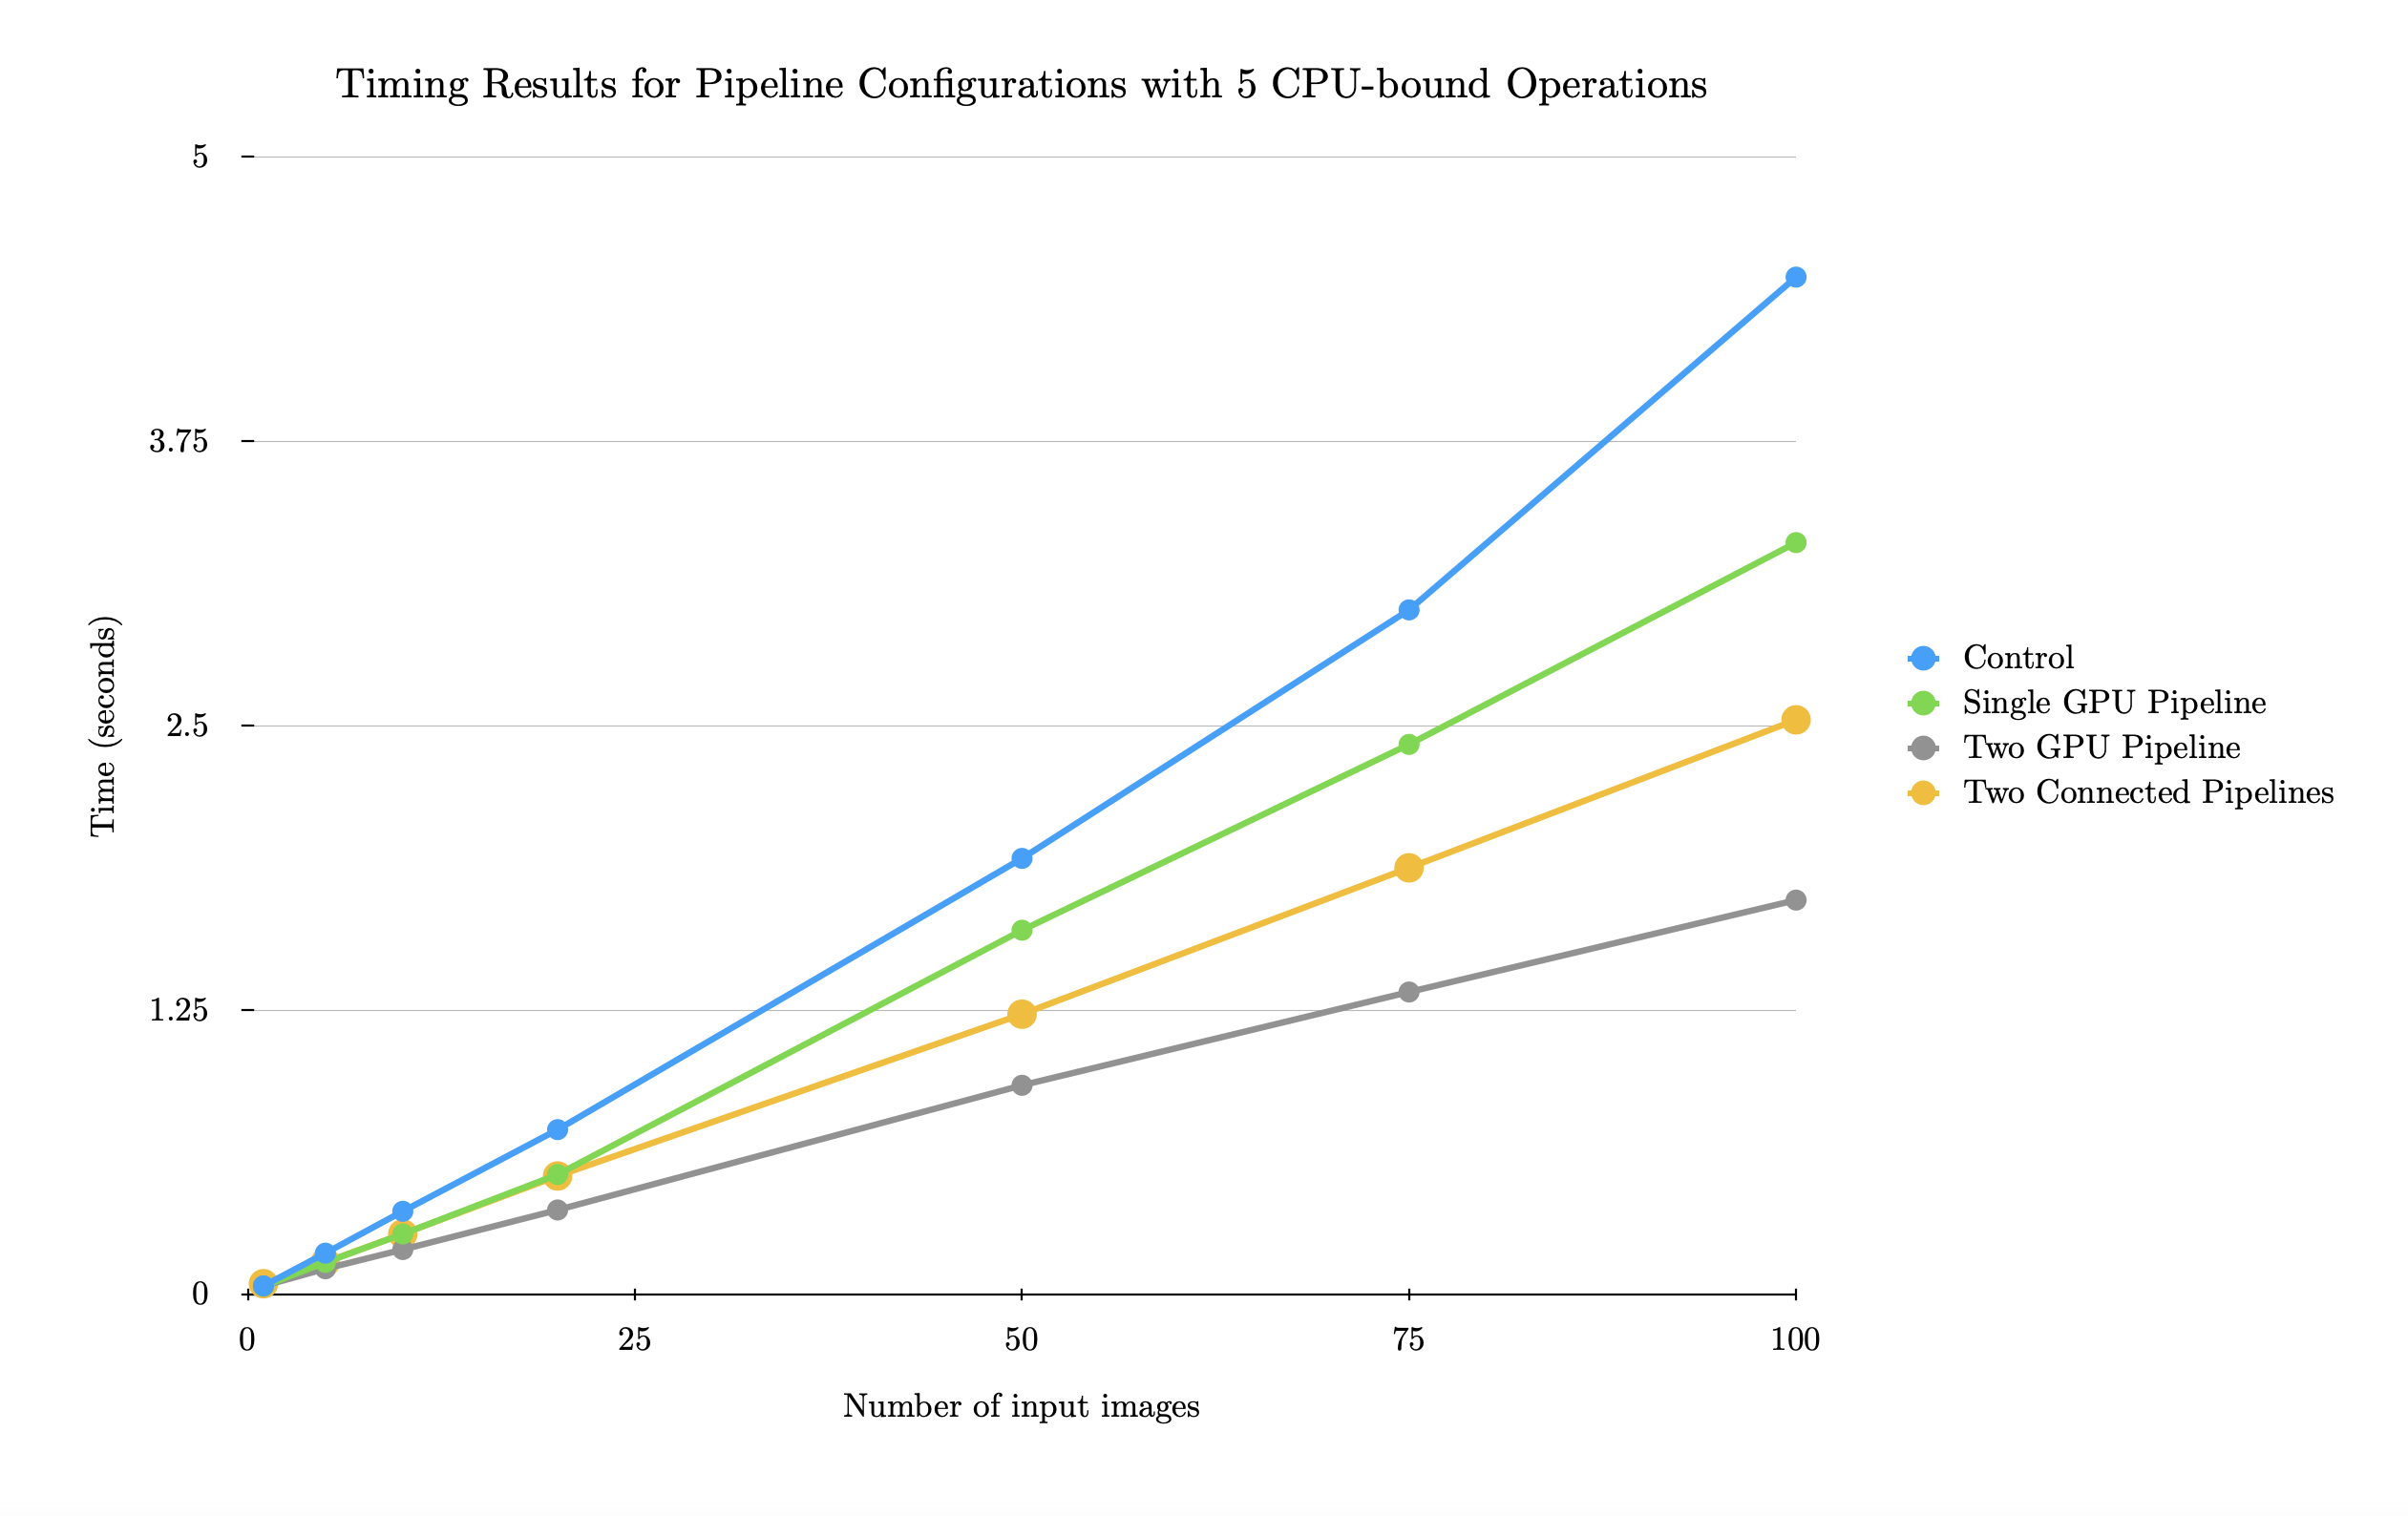
\includegraphics[width=\textwidth]{figures/pipelineChart3.png}
\centering
\caption{Timing results for running a 5-Operation pipeline with simulated CPU-bound pre-processing work.}
\label{pipelineChart2}
\end{figure}

As shown in Table \ref{pipelineTable2} and Figure \ref{pipelineChart2}, these results were more dramatic than the prior five-operation Pipeline experiment. The single-GPU pipeline was able to more predictably outperform the control experiment. We still saw strong performance gains from both of the two-GPU configurations. Despite this, the connected Pipelines still under-performed due to the cost of transferring the work from one Pipeline to the next.

\subsection{Pipelines with 20 Operations}

Lastly, an experiment was performed to see the effects of having longer Pipelines with many Operations. Each Pipeline in this test performed the same 20 Operations: seven Gaussian blurs, four gamma adjustments, two horizontal flips, six 45-degree rotations, and one greyscale conversion. This test is meant to represent more intensive GPU-operations that should further outweigh the costs incurred by the Pipeline's own overhead. For the two connected Pipelines, this work was split down the middle so that each Pipeline performed 10 Operations. 

\begin{table}[H]
\centering
\begin{tabular}{ |c|c|c|c|c| } 
\hline
Number of inputs & Control & Single GPU & Dual GPUs & Connected GPUs \\
\hline
1&	0.1210601&	0.1236825&	0.1229053&	0.1325121\\
5&	0.6136912&	0.6081436&	0.4897915&	0.5424913\\
10&	1.2329561&	1.2234442&	0.7826877&	0.8564503\\
20&	3.2071803&	2.9295116&	1.6075147&	1.6007919\\
50&	14.1225833&	17.9376053&	4.3081120&	4.4900887\\
75&	30.5186737&	30.8800205&	8.4228492&	8.4681248\\
100&	48.8984402&	46.5367387&	14.6403225&	14.5740577\\
\hline
\end{tabular}
\caption{Timing results for running a long 20-Operation Pipeline.}
\label{pipelineTable3}
\end{table}

\begin{figure}[H]
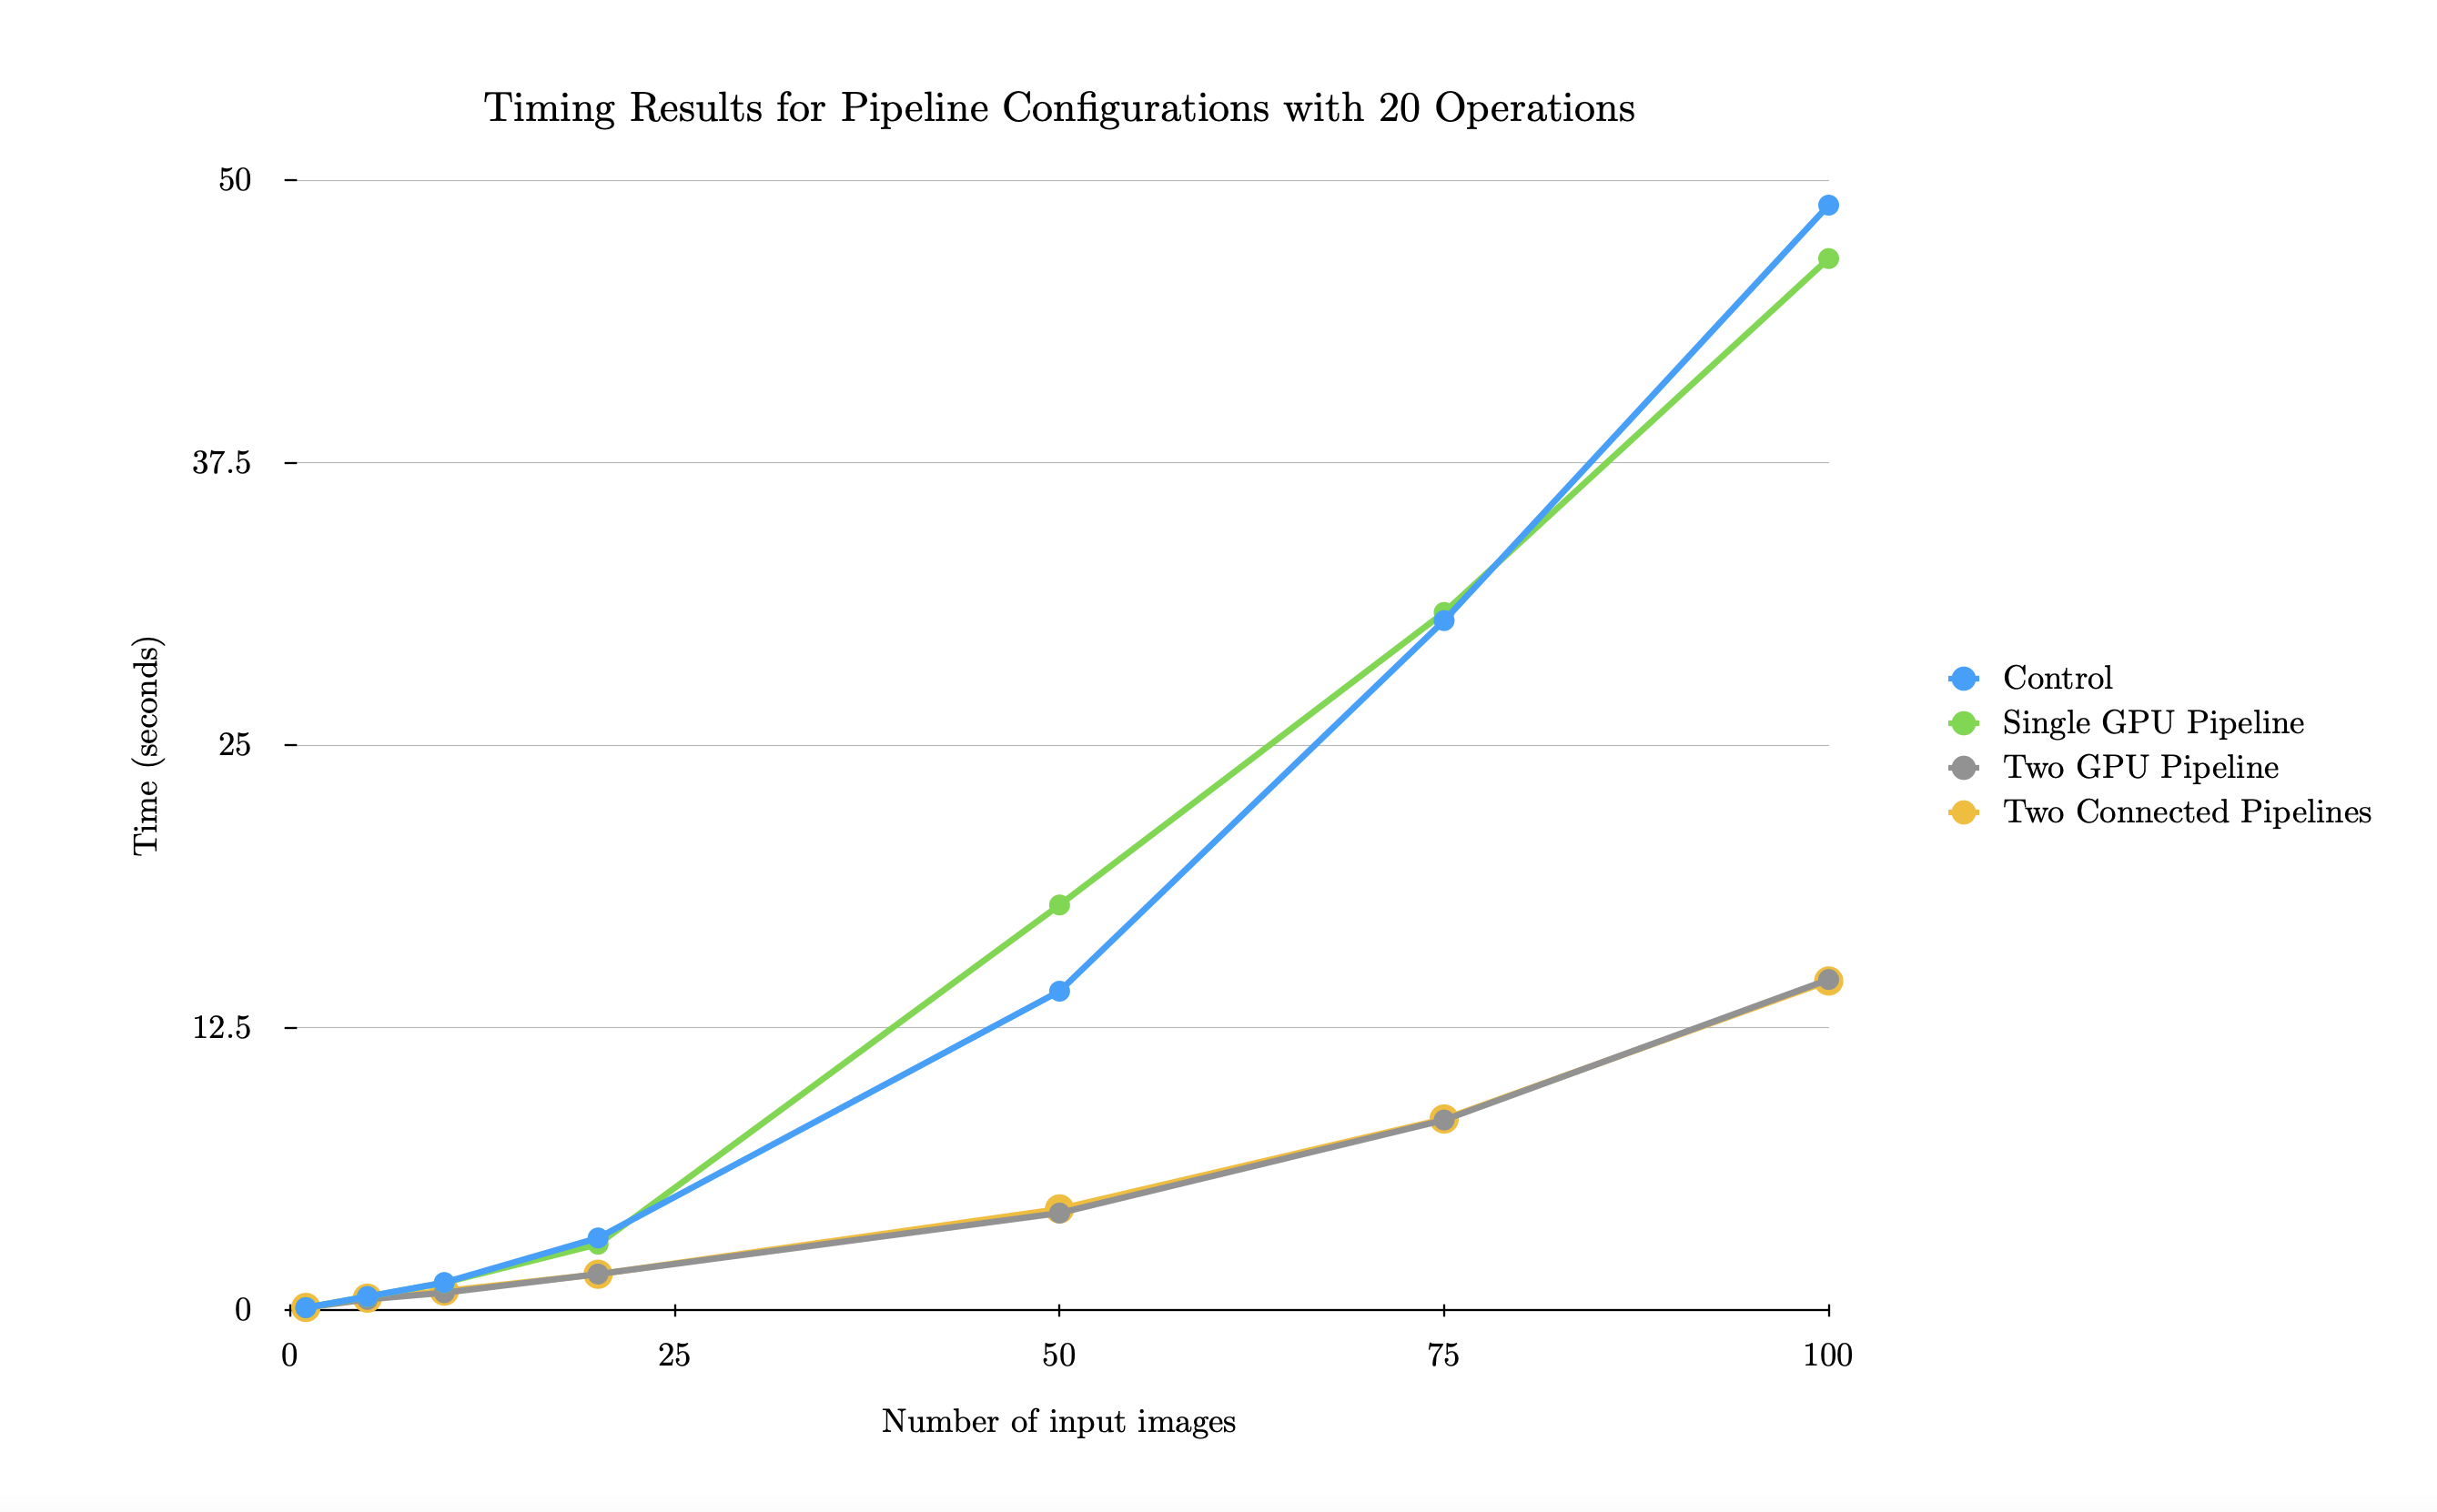
\includegraphics[width=\textwidth]{figures/pipelineChart2.png}
\centering
\caption{Graphical results for running a long 20-Operation Pipeline.}
\label{pipelineChart3}
\end{figure}

\quad As seen in Table \ref{pipelineTable3} and Figure \ref{pipelineChart3}, this experiment produced the most dramatic results. Now that the costs of Pipeline transfer were outweighed by the costs of the GPU computations, both dual-GPU configurations were able to perform roughly the same -- almost always within 0.1 seconds of each other. Surprisingly, both the control and the single-GPU pipeline performed poorly with more than double the runtime of their dual-GPU equivalents. 

\chapter{Conclusion and Discussion}

This thesis has presented the start to a Python GPU programming framework called Millipyde. Millipyde specializes in problems that involve many transformations are performed on array-like input data sets, as is the case with image augmentation. Millipyde also takes takes full advantage of multi-device scheduling in systems that contain more than one GPU. Python programmers who use Millipyde are given the flexibility to let the framework schedule tasks across the available devices, or they can take the reigns themselves with specifying the target device in a variety of situations. Finally, Millipyde was designed in AMD's ROCm platform from the ground up with the goal of providing cross-platform support. 

\quad Millipyde provides two new types for Python programmers -- the gpuarray and the gpuimage. In order to maintain as much compatibility as possible in a complicated landscape of existing Python tools and libraries, these types aim to be fully compatible with NumPy ndarrays and related types such as SciPy's ndimage. Each of these types can be used with a variety of individual functions that take advantage of GPU acceleration. Millipyde also provides execution constructs, the Operation, Pipeline, and the Generator, that allow users to transform data in a variety of ways. Each of these constructs also allows for different scheduling patterns using the available devices on the system.

\quad Our benchmarks showed a lot of promise with Millipyde's performance. The some of the GPU-accelerated functions were able to perform up to tens to hundreds of times faster than their respective CPU variants depending on the task and the size of the input. From there, further acceleration can be achieved by taking advantage of all resources available on the system. Constructs such as the Pipeline can exploit multiple levels of GPU parallelism by using streams on individual GPUs and transferring work across multiple GPUs. In some cases, the performance benefits were less than expected and sometimes resulted in strange benchmarking patterns. More work needs to be done to analyze the program execution in these cases to look for unexpected bottlenecks or data dependencies. More work also needs to be done on experimenting with data types. It's possible that alternative types such as smaller floating point and reducing type conversions values might have improve performance for some functions.

\quad Overall, ROCm proved itself to be a flexible and powerful choice for Millipyde's development. The benefits to cross-platform development are undeniable, and we hope that this becomes the norm for GPU tools and ecosystems going forward. The open nature of the ROCm community allowed us to track down many implementation nuances, bugs, and future plans that may have been harder to find in a closed ecosystem. We hope that AMD stays committed to its view of the future of GPGPU computing, and that more developers join this vision by contributing libraries to the ROCm ecosystem. 

\quad The use of ROCm was not without downsides, however. Due to its infancy, the tools available may not be as powerful as equivalents in environments such as CUDA. One area this showed the most was with benchmarking and profiling. The current profilers proved difficult to use and hard to parse, so we hope that this area gets more attention from developers going forwards.


\chapter{Directions for Future Work}

Millipyde is still only the beginning of a new framework. Over the course of its development, it more often raised questions about modeling GPU programming than it did answer existing questions. There are a variety of directions Millipyde can be taken in going forward -- both in regards to enhancing the current functionality and expanding into new functionality. This chapter will discuss some of these potential directions with the hopes that some of them will be tackled in future iterations of the framework.

\section{Parameter Tuning}

By nature, GPU acceleration involves tuning and micro-benchmarking in order to achieve the best results. It often involves finding the right balance of parameters such as grid/block dimensions, shared memory utilization, memory access patterns, and more. For Millipyde, these parameters were chosen based on the result of tests performed on our experimental AMD workstation. The parameters were then hard-coded into the Millipyde code-base. In practice, these values are likely to vary across different machines with different hardware configurations. This is especially true as new generations of GPUs are released. The trade-offs we made today may not necessarily be the same trade-offs that would give us optimal performance in the future.

\quad Ideally, Millipyde should adapt to new environments and tune its parameters accordingly. A basic approach might be to analyze the properties of the devices that are recognized during module initialization. The framework can use these values to make educated guesses about what parameters to use in executing device kernels. A more sophisticated approach could leverage runtime analysis to make decisions and change parameter values once a kernel has completed. For efficiency, it would be important to cache these values so that they do not need to be re-computed each time a Millipyde program is run. It may be possible to do this using the built-in \verb|__pycache__| folder.

\section{Runtime Scheduling Analysis}

Millipyde makes scheduling decisions using two main steps. The first is to pick the best devices available to use. If a problem is not going to use all available devices, it selects from the available devices using their clock frequencies and maximum supported compute units. The second step is to attempt to divide up the task evenly by distributing work to these devices. This means that Millipyde does not take into account any changes that could happen during runtime. In the future, Millipyde should have a way of monitoring the actual metrics of each device while scheduling tasks. If one device is low on available global memory, for example, then the framework should choose other devices for use in allocating new objects. If one device is shown to have better runtime performance than another, Millipyde should factor that in when making scheduling decisions. And ideally, Millipyde should be able to move around tasks and data during runtime to respond to changes as they happen.

\section{Multiprocess Utilization}

Due to the GIL and limitations on Python's ability to use threads, many Python programs instead turn to multiprocessing as a means of parallel acceleration. This is usually done with the \verb|multiprocessing| package that includes objects such as the \verb|Pool| and \verb|Process| for organizing execution as well as objects such as the \verb|Queue| for exchanging data. In the future, it seems natural for Millipyde to support these abstractions of process-based parallelization in its own framework. Ideally, GPU-based tasks can be assigned to different processes, and integration with the existing Python means of inter-process communication can enhance the tools that Millipyde has for exchanging data. This could provide large benefits to any Millipyde users that are already familiar with Python's model of processing. 

\section{Multi-node Utilization}

Another layer of abstraction that Millipyde could exploit for asynchronous execution is multiple nodes in a computing cluster. As it is today, Millipyde is only able to recognize devices connected to the current system and perform intra-node levels of data transfer. Although this is fine for many problems, GPUs are extremely prevalent in multi-node computing clusters so this remains a huge area for potential future expansion. Although it would likely require large changes to the Millipyde backend, it would allow Millipyde users to tackle larger problems than would otherwise be supported. Since Millipyde is based on the ROCm ecosystem, it would be natural to experiment with ROCm's current tools for inter-node communication. These include the Unified Communication X (UCX) library, and the OpenMPI message passing specification. This would open up many new questions about how work can be scheduled and how systems can be analyzed both during module initialization and during runtime to intelligently distribute work to available nodes and devices. 

\section{Support for User-Defined Kernels}

Currently, all Millipyde GPU kernels are built into the back-end source code itself as pre-defined functions with Python interface wrappers. To make Millipyde as flexible as possible, it should one day cater to the needs of developers who want to write their own GPU-accelerated functions. Many libraries such as CuPy, PyCUDA, and PyOpenCL have experimented with approaches involving Python strings containing GPU kernels written in CUDA C++ syntax that can be then compiled and used in the Python runtime. NVIDIA has taken a similar approach with Python CUDA initiatives announced in 2021 \cite{cudaPython}. Many opportunities still exist for finding new ways of allowing Python users to define their own GPU-accelerated functions. Ideally, future solutions would not require Python users to have to know how to write C++ syntax for kernels, and they should carry on Millipyde's goal of cross-platform flexibility. How these functions can be created and designed from within Python remains an open problem for future work.

\section{Integration with other libraries}

Python libraries seldom exist in a vacuum. One of the great things about Python is how libraries such as NumPy can become the foundation to many new libraries and frameworks that tackle difficult computing problems. Millipyde aims to join these communities and open ecosystems by providing an inter-operable tool for GPU computing. Going forward, more work can be done with exploring interactions between Millipyde and other frameworks and libraries. CuPy, for example, contains many GPU-accelerated functions and tools that can benefit Millipyde's own framework offerings. Another library, Dask, provides NumPy compatible data analysis, data scheduling, and compute-cluster capabilities. These features could be combined with Millipyde's own computing constructs to provide better scheduling and analytics for GPU-based tasks. And these libraries are just the tip of the iceberg. There are many more exciting possibilities for where Millipyde can fit into the ever-growing landscape of Python computing.
\definecolor{dkgreen}{rgb}{0,0.6,0}
\definecolor{gray}{rgb}{0.5,0.5,0.5}
\definecolor{mauve}{rgb}{0.58,0,0.82}
\definecolor{backcolour}{rgb}{1,1,1}

\lstset{frame=none,
    backgroundcolor=\color{backcolour}, 
  language=Python,
  aboveskip=5mm,
  belowskip=5mm,
  showstringspaces=false,
  columns=flexible,
  basicstyle={\linespread{0.8}\small\ttfamily},
  numbers=none,
  numberstyle=\tiny\color{gray},
  keywordstyle=\color{dkgreen},
  commentstyle=\color{blue},
  stringstyle=\color{mauve},
  breaklines=false,
  breakatwhitespace=true,
  tabsize=3
}

\chapter{Millipyde API}

This section will explain the Millipyde API that is exposed to Python developers who use the framework. The following are the imports used in our API example, including the `millipyde' package itself that has been imported as `mp.'

\begin{lstlisting}
import numpy as np
from skimage.io import imsave, imread
import millipyde as mp
\end{lstlisting}

%========================================================================================================================================
\section{gpuarray}

\subsection{Construction}

\begin{description}
   \item[Description] Creates a gpu-compatible array that is inter-operable with NumPy \verb|ndarray|s other \verb|ndarray| compatible types and libraries. 
   \item[Parameters] An array-compatible type. Including but not limited to Numpy \verb|ndarrays|, SciPy \verb|ndimages|, and Python's built-in List Type
   \item[Returns] A \verb|gpuarray| instance
   \item[Raises] \phantom{}
   \begin{itemize}
   \item ValueError if the argument is not array-compatible
   \item ValueError if the array's contents are not a numeric type
   \end{itemize}
   \item[Example] \phantom{}
   \begin{lstlisting}
numpy_array = np.array([1, 2, 3, 4])
gpu_array = mp.gpuarray(numpy_array)

numpy_array2 = np.array([[[1, 2, 3], [4, 5, 6]], 
                         [[1, 2, 3], [4, 5, 6]]])
gpu_array2 = mp.gpuarray(numpy_array2)
                                
gpu_array3 = mp.gpuarray([1, 2, 3, 4])
\end{lstlisting}
\end{description}

\subsection{Methods}

\subsubsection{clone}

\begin{description}
   \item[Description] Clone the \verb|gpuarray|. Creates a deep copy so that all memory is unique. The clone's memory may not be on the same GPU device depending on what device is targeted when the copy is created
   \item[Parameters] None
   \item[Returns] A new \verb|gpuarray|
   \item[Raises] None
   \item[Example] \phantom{}
   \begin{lstlisting}
numpy_array = np.array([1, 2, 3, 4])
gpu_array = mp.gpuarray(numpy_array)
gpu_array2 = gpu_array.clone()
\end{lstlisting}
\end{description}

%========================================================================================================================================

\section{gpuimage}

The \verb|gpuimage| type is a subtype of \verb|gpuarray|. All \verb|gpuarray| functions can accept a \verb|gpuimage| as an argument. The \verb|gpuimage| imposes additional dimensional and type constraints, however, so not all \verb|gpuimage| functions can accept all \verb|gpuarray|s.

\subsection{Construction}

\begin{description}
   \item[Description] Creates a gpu-compatible array representing an image. Construction requires either a 2-dimensional array of float values for greyscale images, or a 3-dimensional array of integer values for colored images. The inner most array dimension in colored images can either be 3 elements wide for RGB images, or 4 elements wide for RGBA images such as PNG files.
   \item[Parameters] An array-compatible type. Including but not limited to NumPy \verb|ndarrays|, SciPy \verb|ndimages|, and Python's built-in List Type.
   \item[Returns] A \verb|gpuarray| instance
   \item[Raises] \phantom{}
   \begin{itemize}
       \item ValueError if the argument is not array-compatible
       \item ValueError if the array's contents are not a numeric type
       \item ValueError if the dimensions don't match greyscale or RGB/RGBA images
   \end{itemize}
   \item[Example] Creating two images in two ways\phantom{}
   \begin{lstlisting}
img = mp.gpuimage(io.imread("images/charlie.png"))

array = np.array([[[64, 76, 32], [22, 65, 64]], 
                  [[12, 53, 43], [33, 56, 42]]])
img2 = mp.gpuimage(array)
\end{lstlisting}
\end{description}

\subsection{Methods}

\subsubsection{rgb2grey}

\begin{description}
   \item[Description] Turns the given rgb or rgba image into a greyscale image represented by floating point values between 0 and 1 for each pixel.
   \item[Parameters] None
   \item[Returns] None
   \item[Raises] None
   \item[Example] Equivalent ways to greyscale a single image
   \begin{lstlisting}
img = mp.gpuimage(io.imread("images/charlie.png"))
img.rgb2grey()
# or
img.rgb2gray()
# or
img.rgba2grey()
# or
img.rgba2gray()
\end{lstlisting}
\end{description}

\subsubsection{transpose}

\begin{description}
   \item[Description] Rotates a \verb|gpuimage| 90\textdegree \ counterclockwise using a transposition operation on the GPU.
   \item[Parameters] None
   \item[Returns] None
   \item[Raises] None
   \item[Example] \phantom{}
   \begin{lstlisting}
img = mp.gpuimage(io.imread("images/charlie.png"))
charlie2.transpose()
\end{lstlisting}
\end{description}

\subsubsection{gaussian}

\begin{description}
   \item[Description] Blur a \verb|gpuimage| using a Gaussian function. A clamping value of 0 is used for calculation involving pixels past the edge of the image.
   \item[Parameters] \phantom{}
   \begin{itemize}
   \item sigma: An integer or float value to use as standard-deviation in the calculation of the convolution kernel
   \end{itemize}
   \item[Returns] None
   \item[Raises] None
   \item[Example] \phantom{}
   \begin{lstlisting}
img = mp.gpuimage(io.imread("images/charlie.png"))
charlie2.gaussian(2)
\end{lstlisting}
\end{description}

\subsubsection{random\_gaussian}

\begin{description}
   \item[Description] Blur a \verb|gpuimage| using a Gaussian function using a random standard deviation in a given range. A clamping value of 0 is used for calculation involving pixels past the edge of the image.
   \item[Parameters] \phantom{}
   \begin{itemize}
   \item min\_sigma: An integer or float value to use as the minimum standard-deviation in the calculation of the convolution kernel
   \item max\_sigma: An integer or float value to use as the maximum standard-deviation in the calculation of the convolution kernel
   \end{itemize}
   \item[Returns] None
   \item[Raises] None
   \item[Example] \phantom{}
   \begin{lstlisting}
img = mp.gpuimage(io.imread("images/charlie.png"))
charlie2.random_gaussian(0, 0.5)
\end{lstlisting}
\end{description}

\subsubsection{brightness}

\begin{description}
   \item[Description] Adjust the brightness of a \verb|gpuimage| by adding the percent change specified by the delta
   \item[Parameters] \phantom{}
   \begin{itemize}
   \item delta: A float value between -1 and 1 for how much to change the brightness by. 
   \end{itemize}
   \item[Returns] None
   \item[Raises] \phantom{}
   \begin{itemize}
       \item ValueError if the delta value is not between -1 and 1 
   \end{itemize}
   \item[Example] \phantom{}
   \begin{lstlisting}
img = mp.gpuimage(io.imread("images/charlie.png"))
img.brightness(.2)
\end{lstlisting}
\end{description}

\subsubsection{random\_brightness}

\begin{description}
   \item[Description] Adjust the brightness of a \verb|gpuimage| by adding the percent change specified by a random delta in the given range
   \item[Parameters] \phantom{}
   \begin{itemize}
   \item min\_delta: A float value between -1 and 1 for the minimum amount to change the brightness by.
   \item max\_delta: A float value between -1 and 1 for the maximum amount to change the brightness by. 
   \end{itemize}
   \item[Returns] None
   \item[Raises] \phantom{}
   \begin{itemize}
       \item ValueError if either the maximum or minimum delta values are not between -1 and 1 
   \end{itemize}
   \item[Example] \phantom{}
   \begin{lstlisting}
img = mp.gpuimage(io.imread("images/charlie.png"))
img.random_brightness(-.2, .5)
\end{lstlisting}
\end{description}

\subsubsection{colorize}

\begin{description}
   \item[Description] Adjust the color of a non-greyscale \verb|gpuimage| multiplying the RGB components by the given multipliers
   \item[Parameters] \phantom{}
   \begin{itemize}
   \item r\_mult: A float value for how much the red value is multiplied by
   \item g\_mult: A float value for how much the green value is multiplied by
   \item b\_mult: A float value for how much the blue value is multiplied by
   \end{itemize}
   \item[Returns] None
   \item[Raises] None
   \item[Example] \phantom{}
   \begin{lstlisting}
img = mp.gpuimage(io.imread("images/charlie.png"))
# Boost the red value and leave green and blue as-is
img.colorize(1.2, 1, 1)
\end{lstlisting}
\end{description}

\subsubsection{random\_colorize}

\begin{description}
   \item[Description] Adjust the color of a non-greyscale gpuimage multiplying the RGB components by random multipliers in the given ranges
   \item[Parameters] \phantom{}
   \begin{itemize}
   \item r\_range: A list of two float values representing a lower and upper bound for how much the red value is multiplied by
   \item g\_range: A list of two float values representing a lower and upper bound for how much the green value is multiplied by
   \item b\_range: A list of two float values representing a lower and upper bound for how much the blue value is multiplied by
   \end{itemize}
   \item[Returns] None
   \item[Raises] None
   \item[Example] \phantom{}
   \begin{lstlisting}
img = mp.gpuimage(io.imread("images/charlie.png"))
img.colorize([.5, 1.5], [.5, 1.5], [.5, 1.5])
\end{lstlisting}
\end{description}

\subsubsection{fliplr}

\begin{description}
   \item[Description] Flip the \verb|gpuimage| left-to-right
   \item[Parameters] None
   \item[Returns] None
   \item[Raises] None
   \item[Example] \phantom{}
   \begin{lstlisting}
img = mp.gpuimage(io.imread("images/charlie.png"))
img.fliplr()
\end{lstlisting}
\end{description}

\subsubsection{rotate}

\begin{description}
   \item[Description] Rotate the \verb|gpuimage| counter-clockwise by the given angle
   \item[Parameters] \phantom{}
   \begin{itemize}
   \item angle: An integer or float value for the rotation angle in degrees
   \end{itemize}
   \item[Returns] None
   \item[Raises] None
   \item[Example] \phantom{}
   \begin{lstlisting}
img = mp.gpuimage(io.imread("images/charlie.png"))
# Rotate 5 degrees counter-clockwise
img.rotate(5)
\end{lstlisting}
\end{description}

\subsubsection{random\_rotate}

\begin{description}
   \item[Description] Rotate the \verb|gpuimage| counter-clockwise by a random angle within the given range
   \item[Parameters] \phantom{}
   \begin{itemize}
   \item min\_angle: An integer or float value for the minimum rotation angle in degrees
   \item max\_angle: An integer or float value for the maximum rotation angle in degrees
   \end{itemize}
   \item[Returns] None
   \item[Raises] None
   \item[Example] \phantom{}
   \begin{lstlisting}
img = mp.gpuimage(io.imread("images/charlie.png"))
# Rotate randomly between 45 and 180 degrees counter-clockwise
img.random_rotate(45, 180)
\end{lstlisting}
\end{description}

\subsubsection{adjust\_gamma}

\begin{description}
   \item[Description] Perform gamma correction on the \verb|gpuimage|
   \item[Parameters] \phantom{}
   \begin{itemize}
   \item gamma: An float value for gamma
   \item gain: A float value for gain that is used as a constant multiplier
   \end{itemize}
   \item[Returns] None
   \item[Raises] None
   \item[Example] \phantom{}
   \begin{lstlisting}
img = mp.gpuimage(io.imread("images/charlie.png"))
# 2nd Power gamma with standard gain
img.adjust_gamma(2, 1)
\end{lstlisting}
\end{description}

\subsubsection{random\_adjust\_gamma}

\begin{description}
   \item[Description] Perform a random gamma correction on the \verb|gpuimage|
   \item[Parameters] \phantom{}
   \begin{itemize}
   \item gamma\_range: A list of two float values representing a lower and upper bound for gamma
   \item gain\_range: A list of two float values representing a lower and upper bound for gain
   \end{itemize}
   \item[Returns] None
   \item[Raises] None
   \item[Example] \phantom{}
   \begin{lstlisting}
img = mp.gpuimage(io.imread("images/charlie.png"))
img.adjust_gamma([2, 3], [1, 1.2])
\end{lstlisting}
\end{description}

\subsubsection{clone}

\begin{description}
   \item[Description] Clone the \verb|gpuimage|. Creates a deep copy so that all memory is unique. The clone's memory may not be on the same GPU device depending on what device is targeted when the copy is created
   \item[Parameters] None
   \item[Returns] A new \verb|gpuimage|
   \item[Raises] None
   \item[Example] \phantom{}
   \begin{lstlisting}
img = mp.gpuimage(io.imread("images/charlie.png"))
img2 = img.clone()
\end{lstlisting}
\end{description}

\subsection{Related Module Functions}

\subsubsection{image\_from\_path}

\begin{description}
   \item[Description] Create a \verb|gpuimage| using the image file located at the given path
   \item[Parameters] \phantom{}
   \begin{itemize}
       \item path: A string path for a specific image file. The file must be an appropriate image format such as PNG, JPEG, TIFF, BPM, etc.
   \end{itemize}
   \item[Returns] A new \verb|gpuimage|
   \item[Raises] None
   \item[Example] \phantom{}
   \begin{lstlisting}
# Load from the local images directory
img = image_from_path("images/charlie.png")
\end{lstlisting}
\end{description}

\subsubsection{images\_from\_path}

\begin{description}
   \item[Description] Create a list of \verb|gpuimages| using the all image files located at the given path
   \item[Parameters] \phantom{}
   \begin{itemize}
       \item path: A string path containing the images to load. Files that are not an appropriate image format will be ignored.
   \end{itemize}
   \item[Returns] A new list of \verb|gpuimages|
   \item[Raises] None
   \item[Example] \phantom{}
   \begin{lstlisting}
# Load from the local images directory
img = images_from_path("images/")
# Paths can also exclude the final slash
img = images_from_path("images")
\end{lstlisting}
\end{description}

%========================================================================================================================================

\section{Device}

The Device type can be used in coordination with Python \verb|with| statements to set which target device is used within a given scope. At exit, the \verb|with| statement will return the target Device back to the one used before the \verb|with| call. When exiting the scope, Millipyde will synchronize with the target Device to make sure all work has finished. In the case of an error with the Device, the device will be reset so that the exception thrown can be caught if desired and the target Device can be used in future calls. These \verb|with| statements can also be nested to use specific devices in specific situations and to safely return back to the previous target device when back in the outer \verb|with| statement's scope.

\subsection{Construction}

\begin{description}
   \item[Description] Creates a scope that uses a specific device ID as the gpu device to target. All types constructed inside this scope will use this target for gpu-based memory allocation. Any functions inside the scope will also be executed on the gpu specified by the target Device.
   \item[Parameters] \phantom{}
   \begin{itemize}
       \item device\_id: An integer representing the device ID to use
   \end{itemize}
   \item[Returns] A Device instance
   \item[Raises] Any errors that occur inside the \verb|with| statement
   \item[Example] \phantom{}
   \begin{lstlisting}
with mp.Device(0):
    # img is created on device 0
    img = mp.gpuimage(io.imread("images/charlie.png"))
    with mp.Device(1):
        # img is transferred to device 1 and greyscaled there
        img.rgb2grey()
    # img is transferred back to device 0 and transposed there
    img.transpose()
\end{lstlisting}
\end{description}

\subsection{Related Module Functions}

\subsubsection{get\_current\_device}

\begin{description}
   \item[Description] Get the target Device for the given scope 
   \item[Parameters] None
   \item[Returns] An integer device ID
   \item[Raises] None
   \item[Example] \phantom{}
   \begin{lstlisting}
with mp.Device(0):
    # Returns 0
    d = mp.get_current_device()
    with mp.Device(1):
        # Returns 1
        d = mp.get_current_device()
\end{lstlisting}
\end{description}

\subsubsection{get\_device\_count}

\begin{description}
   \item[Description] Get the number of recognized devices on the system 
   \item[Parameters] None
   \item[Returns] An integer device ID
   \item[Raises] None
   \item[Example] \phantom{}
   \begin{lstlisting}
count = mp.get_device_count()
for i in range(count):
    with mp.Device(i):
        pass
\end{lstlisting}
\end{description}

%========================================================================================================================================

\section{Operation}

\subsection{Construction}

\begin{description}
   \item[Description] Creates an operation around the given function or class method that can be run later
   \item[Parameters] \phantom{}
   \begin{itemize}
       \item function: A callable such as a function or lambda, or a string representing a method name for instance methods
       \item params...: Variable length parameters to be used when calling 'function'
       \item probability [optional]: A float probability between 0 and 1 (exclusive) that is re-evaluated each time this Operation is used to determine whether the function is called
   \end{itemize}
   \item[Returns] An Operation instance
   \item[Raises] \phantom{}
   \begin{itemize}
       \item ValueError for invalid probabilities
   \end{itemize}
   \item[Example] \phantom{}
   \begin{lstlisting}
def add_two_nums(x, y):
    return x + y

# Operation constructed from function in current scope
op = mp.Operation(add_two_nums, 4, 6)

# Operation constructed from instance method
grey_op = mp.Operation("rgb2grey")

# Operation with arguments and probability
gauss_op = mp.Operation("gaussian", 2, probability=.5)

\end{lstlisting}
\end{description}

\subsection{Methods}

\subsubsection{run}

\begin{description}
   \item[Description] Run the given Operation that represents a function. This method cannot run an Operation representing an instance method. See run\_on for more.
   \item[Parameters] None
   \item[Returns] Return the result of calling the function represented by the Operation, or None if the function did not run at all due to its probability
   \item[Raises] \phantom{}
   \begin{itemize}
       \item RuntimeError if the probability calculation fails. This may be due to a system call failure in the random number retrieval
   \end{itemize}
   \item[Example] \phantom{}
   \begin{lstlisting}
def print_hello():
    print("Hello world!")

hello_op = mp.Operation(print_hello, probability=.8)
operation.run()

\end{lstlisting}
\end{description}

\subsubsection{run\_on}

\begin{description}
   \item[Description] Run the given Operation that represents an instance method.
   \item[Parameters]
   \begin{itemize}
       \item instance: The instance to run the instance method on
   \end{itemize}
   \item[Returns] Return the result of calling the instance method represented by the Operation, or None if the function did not run at all due to its probability
   \item[Raises] \phantom{}
   \begin{itemize}
       \item RuntimeError if the probability calculation fails. This may be due to a system call failure in the random number retrieval
       \item ValueError if the given instance does not have this method
   \end{itemize}
   \item[Example] \phantom{}
   \begin{lstlisting}
img = mp.image_from_path("/images/charlie.png")
gauss_op = mp.Operation("gaussian", 2, probability=.5)

gauss_op.run_on(img)

\end{lstlisting}
\end{description}

%========================================================================================================================================

\section{Pipeline}

\subsection{Construction}

\begin{description}
   \item[Description] Creates a Pipeline
   \item[Parameters] \phantom{}
   \begin{itemize}
       \item inputs: A list of gpu-compatible types (gpuarray and/or gpuimage)
       \item operations: a list of Operation types. All Operatons representing instance methods must be able to operate on gpu-types
       \item device [optional]:  An integer representing the ID of the device that the pipeline will execute on. Overrides any targeted device. Will attempt to use all available devices if none is specified and if no target device is set.
   \end{itemize}
   \item[Returns] A Pipeline instance
   \item[Raises] \phantom{}
   \begin{itemize}
       \item ValueError for invalid parameters
   \end{itemize}
   \item[Example] \phantom{}
   \begin{lstlisting}
inputs = [mp.image_from_path("images/charlie.png"),
          mp.image_from_path("images/aspen.png")]

operations = [mp.Operation("colorize", 1.5, .8. 1),
               mp.Operation("transpose"),
               mp.Operation("rgb2grey", probability=0.5)]

# The following pipeline will attempt to use all available devices
p1 = mp.Pipeline(inputs, operations)

# The following pipeline will only schedule on device 1
with mp.Device(1):
    p2 = mp.Pipeline(inputs, operations)

# The following will only schedule on device 0
# It will override target device 1
with mp.Device(1):
    p3 = mp.Pipeline(inputs, operations, device=0)

\end{lstlisting}
\end{description}

\subsection{Methods}

\subsubsection{connect\_to}

\begin{description}
   \item[Description] Connect one Pipeline to another so that the outputs from one become the inputs to the other. They will execute concurrently as soon as any of the outputs are ready from the first pipeline. Millipyde will attempt to find an optimal way of scheduling each Pipeline on a separate device if one or both Pipelines are not specified to use a specific device
   \item[Parameters] \phantom{}
   \begin{itemize}
       \item pipeline: The Pipeline that will accept this Pipeline's results as inputs
   \end{itemize}
   \item[Returns] None
   \item[Raises] None
   \item[Example] \phantom{}
   \begin{lstlisting}
# Letting Millipyde find the best scheduling of devices it can
p = mp.Pipeline(inputs, operations)
p2 = mp.Pipeline([], operations2)
p.connect_to(p2)

# Forcing both pipelines to use specific devices
p = mp.Pipeline(inputs, operations, device=0)
p2 = mp.Pipeline([], operations2, device=1)
p.connect_to(p2)

\end{lstlisting}
\end{description}

\subsubsection{run}

\begin{description}
   \item[Description] Run the Pipeline instance. This function will only return once all inputs have been operated on, and once all connected Pipelines have completed as well. Running a pipeline mutates the inputs.
   \item[Parameters] None
   \item[Returns] None
   \item[Raises] None
   \item[Example] \phantom{}
   \begin{lstlisting}
p1 = mp.Pipeline(inputs, operations)
p2 = mp.Pipeline([], operations2)
p3 = mp.Pipeline([], operations3)
p1.connect_to(p2)
p2.connect_to(p3)

# Returns once p1, p2, and p3 have completed
p.run()

\end{lstlisting}
\end{description}

%========================================================================================================================================

\section{Generator}

\subsection{Construction}

\begin{description}
   \item[Description] Creates a Generator with the given inputs and operations
   \item[Parameters] \phantom{}
   \begin{itemize}
       \item inputs: A list of gpu-compatible types (gpuarray and/or gpuimage), or a string path that contains images that can be turned into gpuimages
       \item operations: a list of Operation types. All Operations representing instance methods must be able to operate on gpu-types
       \item device [optional]: An integer representing the ID of device that the Generator will execute on. Overrides any targeted device. Will attempt to use the best available device if none is specified and no target was specified for this scope.
       \item outputs [optional]: An integer representing the amount of outputs to create. The output set size will be infinite if none is specified
       \item return\_to\_host [optional]: A boolean value for whether or not the results should be automatically turned into NumPy ndarrays. 
   \end{itemize}
   \item[Returns] A Generator instance
   \item[Raises] \phantom{}
   \begin{itemize}
       \item ValueError for invalid parameters
       \item StopIteration if we have generated all specified outputs
   \end{itemize}
   \item[Example] \phantom{}
   \begin{lstlisting}
operations = [mp.Operation("colorize", 1.5, .8. 1),
               mp.Operation("transpose"),
               mp.Operation("rgb2grey", probability=0.5)]

# Will produce 3 outputs using device 1
g1 = mp.Generator("examples/images", operations, 
        return_to_host=True, outputs=3, device=1)

i = 1
for result in g1:
    imsave("output" + str(i) + ".png", result)
    i += 1
    
# Will produce N number of outputs on the best available device
g1 = mp.Generator("examples/images", operations, return_to_host=True)

for i in range(n):
    result = next(g)
    imsave("output" + str(i) + ".png", result)

\end{lstlisting}
\end{description}


\nocite{*}
\bibliography{bibliography}

% Indents Appendix in Table of Contents
\makeatletter
\addtocontents{toc}{\let\protect\l@chapter\protect\l@section}
\makeatother

% Hack to make Appendices to appear in Table of Contents
%\addtocontents{toc}{%
%   \noindent APPENDICES
%}
%\begin{appendices}
%

%\end{appendices}

\end{document}
